\documentclass[a4paper, 12pt, openany]{book} %chose the paper size and font size. Openany ensures that all all chapters and similar may begin at any page, not only odd pages. For the introductory pages and appendices we want openany, but for chapter pages in the main content we want chapters to begin only on odd pages (right hand side). The book class ensures that the margins are automatically adjusted such that left hand pages are slightly moved to the left and vice versa at the right, which makes the thesis very readable and good looking when printed in bound book format.

\usepackage[nottoc]{tocbibind}
\usepackage[utf8]{inputenc}
\usepackage[T1]{fontenc}
\usepackage[Bjarne]{fncychap}
\usepackage{fancyhdr}
\usepackage[lmargin=1.5in, rmargin=1in, tmargin=1in, bmargin=1in]{geometry}
\usepackage{url}
\usepackage{listings}
\usepackage{amsmath,amssymb}
\usepackage{array}
\usepackage{multirow}
\usepackage{siunitx}
\usepackage[bf]{caption}
\usepackage{subcaption}
\usepackage{array, booktabs}
\usepackage{graphicx}
\usepackage{float}
\usepackage[export]{adjustbox}
\usepackage{subfig}
\usepackage{chngcntr}
\usepackage{color, xcolor}
\usepackage{comment}
\usepackage{afterpage}
\usepackage{siunitx}
\usepackage[backend = biber,
            style = ieee,
            date = long,
            urldate = iso8601,
            sorting = none,
            maxcitenames = 3,
            giveninits=false % Does NOT include initials
            ]{biblatex}
\usepackage{pgfplots}
\usepackage{pdfpages}
\usepackage[colorlinks=true, allcolors=black]{hyperref}
\usepackage[toc, acronyms]{glossaries}

\usepgfplotslibrary{external}
\tikzexternalize


%%%%%%%%%%%%%%%%%%%%%%%%% CONFIG %%%%%%%%%%%%%%%%%%%%%%%%%

% \renewbibmacro*{urldate}{
%     (Accessed:  \printfield{urlday}.\printfield{urlmonth}.\printfield{urlyear})
% }

\DeclareFieldFormat{urldate}{(Accessed: \thefield{urlday}.\addspace
  \mkbibmonth{\thefield{urlmonth}}\addspace
  \thefield{urlyear}\isdot)}

\setcounter{tocdepth}{2}
\setcounter{secnumdepth}{4}

% \counterwithin{figure}{section}
% \counterwithin{table}{section}

\bibliography{references}

\newcommand\MyBox[2]{
  \fbox{\lower0.75cm
    \vbox to 1.7cm{\vfil
      \hbox to 1.7cm{\hfil\parbox{1.4cm}{#1\\#2}\hfil}
      \vfil}%
  }%
}

\newcommand\myemptypage{
    \null
    \thispagestyle{empty}
    \addtocounter{page}{-1}
    \newpage
}

\newcommand{\saleh}[0]{Saleh Abdel-Afou Alaliyat}
\newcommand{\arne}[0]{Arne Unneland}
\newcommand{\peter}[0]{Peter Batchelor}
\newcommand{\birgitte}[0]{Birgitte Louise Vik Thoresen}
\newcommand{\chris}[0]{Chris Sivert Sylte}
\newcommand{\vegard}[0]{Vegard Arnesen Mytting}

%%%%%%%%%%%%%%%%%%%%%%%%% CODE %%%%%%%%%%%%%%%%%%%%%%%%%

\newfloat{code}{htbp}{loc}[section]

\floatname{code}{Code}

\newcommand{\loc}[0]{List of Code}

\newcommand{\listofcode}{\addcontentsline{toc}{chapter}{\loc}\listof{code}{\loc}}

\definecolor{background}{HTML}{FFFFFF}
\definecolor{text}{HTML}{000000}
\definecolor{keyword}{HTML}{0000FF}
\definecolor{string}{HTML}{A31515}
\definecolor{comment}{HTML}{008000}
\definecolor{number}{HTML}{098658}
\definecolor{function}{HTML}{795E26}

\lstset{
    backgroundcolor=\color{background},
    basicstyle=\ttfamily\color{text},
    keywordstyle=\color{keyword},
    stringstyle=\color{string},
    commentstyle=\itshape\color{comment},
    numberstyle=\color{number},
    showstringspaces=false,
    breaklines=true,
    frame=single,
    rulecolor=\color{text},
    tabsize=4,
    captionpos=b,
    escapeinside={(*}{*)},
    morekeywords={function, if, else, return},
    numbers=left,
    numberstyle=\tiny\color{gray},
    numbersep=10pt,
    stepnumber=1,
    firstnumber=1
}

%%%%%%%%%%%%%%%%%%%%%%%%% GLS %%%%%%%%%%%%%%%%%%%%%%%%%

\makeglossaries

\newglossaryentry{check}{
    name={check}, 
    description={A direct threat to the king that the opponent can legally escape from}
}

\newglossaryentry{checkmate}{
    name={checkmate}, 
    description={A position where the king is under attack and cannot escape, ending the game}
}

\newglossaryentry{stalemate}{
    name={stalemate}, 
    description={A situation where the player to move is not in check but has no legal moves; the game is declared a draw}
}

\newglossaryentry{capture}{
    name={capture}, 
    description={The removal of an opponent’s piece from the board as a result of a legal move}
}

\newglossaryentry{castling}{
    name={castling}, 
    description={A special move involving the king and one rook, where the king moves two squares toward the rook and the rook is placed on the square the king crossed}
}

\newglossaryentry{en-passant}{
    name={en passant}, 
    description={A special pawn capture that occurs when an opposing pawn moves two squares forward and lands adjacent; it may be captured as if it had moved only one square}
}

\newglossaryentry{promotion}{
    name={promotion}, 
    description={When a pawn reaches the opponent's back rank, it is converted into a queen, rook, bishop, or knight of the same color (excluding king or another pawn)}
}

\newglossaryentry{stockfish}{
    name={Stockfish}, 
    description={An open-source chess engine considered among the strongest in the world}
}

\newglossaryentry{lichess}{
    name={Lichess}, 
    description={A free, open-source online chess platform for playing, learning, and analyzing games}
}

\newglossaryentry{fide}{
    name={FIDE}, 
    description={The International Chess Federation; the global governing body of chess competitions}
}

\newglossaryentry{elo}{
    name={Elo rating}, 
    description={A system for calculating the relative skill levels of players in zero-sum games like chess}
}

\newglossaryentry{bullet}{
    name={bullet}, 
    description={A chess time control where each player has less than three minutes for the entire game}
}

\newglossaryentry{blitz}{
    name={blitz}, 
    description={A fast-paced chess format with a base time of 3 to 10 minutes per player}
}

\newglossaryentry{rapid}{
    name={rapid}, 
    description={A chess format with a base time of more than 10 minutes but less than 60 minutes per player}
}

\newglossaryentry{classical}{
    name={classical}, 
    description={A traditional chess format where each player has at least 60 minutes for the entire game}
}

\newglossaryentry{back-rank}{
    name={back rank}, 
    description={The first row (rank) on a player's side of the board at the start of the game, containing all major pieces}
}

\newglossaryentry{chess960}{
    name={Chess960}, 
    description={A chess variant, also called Fischer Random, where the starting position of the back-rank pieces is randomized}
}

\newglossaryentry{horde}{
    name={Horde}, 
    description={A chess variant in which White has 36 pawns and Black plays with a standard set of pieces}
}

\newglossaryentry{racing-kings}{
    name={Racing Kings}, 
    description={A chess variant where players race to be the first to move their king to the eighth rank}
}

\newglossaryentry{git}{
    name={Git}, 
    description={A distributed version control system used to track changes in source code during software development}
}

\newglossaryentry{github}{
    name={GitHub}, 
    description={A web-based hosting service for Git repositories that supports collaboration, version control, and code review}
}

\newglossaryentry{repository}{
    name={repository},
    plural={repositories},
    description={A storage location for software code, documentation, and revision history}
}

\newglossaryentry{scrum}{
    name={Scrum}, 
    description={Scrum is a management framework that teams use to self-organize and work towards a common goal}
}

\newglossaryentry{agile}{
    name={Agile}, 
    description={A software development methodology emphasizing iterative delivery, adaptability, and close collaboration}
}

\newglossaryentry{latex}{
    name={LaTeX},
    description={A high-quality typesetting system used for producing technical and scientific documentation}
}

\newglossaryentry{python}{
    name={Python}, 
    description={A high-level, interpreted programming language known for its readability and broad applicability}
}

\newglossaryentry{wireframe}{
    name={wireframe},
    description={A simplified visual representation of a user interface layout, used for planning and structuring applications}
}


%%%%%%%%%%%%%%%%%%%%%%%%% ACR %%%%%%%%%%%%%%%%%%%%%%%%%

\newacronym{ai}{AI}{Artificial Intelligence}

\newacronym{api}{API}{Application Programming Interface}

\newacronym{cpu}{CPU}{Central Processing Unit}

\newacronym{cnn}{CNN}{Convolutional Neural Network}

\newacronym{fen}{FEN}{Forsyth-Edwards Notation}

\newacronym{http}{HTTP}{Hypertext Transfer Protocol}

\newacronym{ide}{IDE}{Integrated Development Environment}

\newacronym{yolo}{YOLO}{You Only Look Once}

\newacronym{leyolo}{LeYOLO}{Lightweight and Efficient You Only Look Once}

\newacronym{onnx}{ONNX}{Open Neural Network Exchange}

\newacronym{nms}{NMS}{Non Maximum Suppression}

\newacronym{llm}{LLM}{Large Language Model}

\newacronym{ml}{ML}{Machine Learning}

\newacronym{lstm}{LSTM}{Long Short-Term Memory}

\newacronym{ntnu}{NTNU}{Norwegian University of Science and Technology}

\newacronym{pgn}{PGN}{Portable Game Notation}

\newacronym{rest}{REST}{Representational State Transfer}

\newacronym{rfid}{RFID}{Radio-frequency Identification}

\newacronym{swc}{SWC}{Speedy Web Compiler}

\newacronym{tcp}{TCP}{Transmission Control Protocol}

\newacronym{tdd}{TDD}{Test-Driven Development}

\newacronym{ui}{UI}{User Interface}

\newacronym{uml}{UML}{Unified Modeling Language}

\newacronym{usb}{USB}{Universal Serial Bus}

\newacronym{ux}{UX}{User Experience}

\newacronym{vm}{VM}{Virtual Machine}

\newacronym{eco}{ECO}{Encyclopaedia of Chess Openings}

\newacronym{otb}{OTB}{over-the-board}

\newacronym{vscode}{VS Code}{Visual Studio Code}

\newacronym{wcag}{WCAG}{Web Content Accessibility Guidelines}




\begin{document}

% \begin{titlepage}
\newgeometry{left=1.6in, right=2in}
\vspace*{1.5cm}

\noindent  \textcolor{gray}{\large 
Birgitte Louise Vik Thoresen \\ 
Chris Sivert Sylte \\ 
Vegard Arnesen Mytting} \\
\vspace{1cm}

\noindent \textbf{\Large Live Digitization of Chess Games} \\
\vspace{0.5cm}

\noindent {\large Digitization of a chess game based on a camera} \\

\vspace{7cm}
\noindent Bachelor's Thesis in Computer Science \\
Supervisor: Saleh Abdel-Afou Alaliyat \\
May 2025 \\

\vspace{0.2cm}
\noindent Norwegian University of Science and Technology \\
Faculty of Information Technology and Electrical Engineering \\
Department of ICT and Natural Sciences \\

\begin{figure}[h]
    
\includegraphics[width=0.28\textwidth]{figures/ntnu_basic.png}
\end{figure}
\end{titlepage}
\restoregeometry
\myemptypage %empty page such that the abstract starts at the first right hand side after the title page

\pagenumbering{roman}

\chapter*{Abstrakt}
\addcontentsline{toc}{chapter}{Abstrakt}

Formålet med dette prosjektet er å utvikle en automatisert løsning for \textbf{Aalesunds Schaklag} som muliggjør kontinuerlig sjakkspilling på et vanlig brett mens du samtidig digitalisere spillet til \gls{pgn}-filer. Digitaliserte spill gjøres tilgjengelige via et \gls{api} ved å strømme bevegelser som hendelser i en meldingskø. Systemet utnytter bildegjenkjenning for å identifisere brettet og brikkene, kombinert med sanntidsvalidering av trekk for å sikre overholdelse av sjakkreglene. \\

Løsningen er designet for å operere på lokal maskinvare, vanligvis med et \acrshort{usb}-tilkoblet webkamera og en lokal maskin (Windows eller Ubuntu), som sikrer at behandling utføres lokalt uten avhengighet av skyinfrastruktur. Mens digitale sjakkbrett som er i stand til lignende funksjonalitet finnes, er de kostbare og er omfattende å sette opp. Dette prosjektet har som mål å gi et kostnadseffektivt og effektivt alternativ ved å automatisere digitaliseringsprosessen. \\

Utviklingsprosessen fulgte smidige metoder, ved å bruke teknologier som \gls{leyolo} og \gls{python} for å implementere systemet. Denne tilnærmingen sikret iterativ fremgang, tilpasningsevne til endrede krav, og levering av en funksjonell og skalerbar løsning. \\

\textbf{*oppsummering av resultat skrives her*}\\

\textbf{*oppsummering av konklusjon skrives her*}


\newpage


\chapter*{Abstract}
\addcontentsline{toc}{chapter}{Abstract}
This project aimed to develop an automated system to digitize \gls{otb} chess games. The system allowed players to use a traditional physical board while their moves were captured and recorded in real time. Image recognition was utilized to detect board states and validate moves according to chess rules. 
The digitized games were displayed in real time through a frontend interface, allowing users to retrieve the PGN or move history of the ongoing game

The solution was designed to run entirely on local hardware, using a USB-connected webcam and a standard Windows or Ubuntu machine, with no reliance on cloud services. Unlike commercial digital chessboards, which are often costly and complex to set up, this system provided a cost-effective and easy-to-deploy alternative.

Development followed agile principles and employed tools such as Python and \acrshort{leyolo} to deliver a functional and scalable prototype. The project demonstrated that affordable, locally hosted digitization of OTB chess games is feasible and practical for clubs and individual users.

\textbf{*recap of the result is written here*}\\

\textbf{*recap of the conclusion is written here*}

\chapter*{Preface}
\addcontentsline{toc}{chapter}{Preface}

This thesis marks the culmination of our bachelor's degree in Computer Science at NTNU Ålesund, completed during the spring semester of 2025. The project has allowed us to apply our theoretical knowledge to a real-world problem, deepening our understanding of machine learning, software development, and agile workflows. We are grateful for the opportunity to work on a project that combines our interests in chess and software development. \\

We would like to extend our sincere gratitude to our supervisor, \textbf{\saleh}, for his invaluable guidance, continuous support, and insightful feedback throughout the duration of this project. His expertise and encouragement have been instrumental in shaping the direction and success of our work. We are also deeply thankful to the product owner, \textbf{\arne}, for providing us with the opportunity to undertake this project and for his constructive feedback, which greatly enhanced the quality of our deliverables. Additionally, we would like to acknowledge the external assistance provided by \textbf{\peter}, whose expertise and support were crucial in overcoming challenges and advancing our project.

%%%%%%%%%%%%%%%%%%%%%%%%% TOC %%%%%%%%%%%%%%%%%%%%%%%%%
\newpage

\addcontentsline{toc}{chapter}{Contents}

\tableofcontents

\listoffigures

\newpage

\listoftables

\newpage

\renewcommand{\acronymname}{Abbreviations}
\printglossary[type=\acronymtype]

\printglossary

%%%%%%%%%%%%%%%%%%%%%%%%%%%%%%%%%%%%%%%%%%%%%%%%%%%%%%%

\newpage
\myemptypage

\pagestyle{fancy} %set customized page style for header
\fancyhf{} %clear header and footer fields
\renewcommand{\headrulewidth}{0pt} %set to no rule
\fancyhead[LE, RO]{\thepage} %set the page number at left for even, right for odd pages
\fancyhead[RE, LO]{\leftmark} %set the chapter name at right for even, left for odd pages
%is is possible to design the header with the chapter as you wish, e.q. only the chapter or only the name, all lowercase instead etc.
%you could also design the footer if you wish, for example:
%\fancyfoot[LE, RO]{\thepage}
\setlength{\headheight}{14.49998pt} %set the header height

%%%%%%%%%%%%%%%%%%%%%%%%%%%%%%%%%%%%%%%%%%%%%%%%%%%%%%%

\pagenumbering{arabic}

\chapter{Introduction}

\begin{center} 
\textit{This chapter presents the background of the project, outlines the objective, defines the requirements, and lists the equipment used.}
\end{center}


\section{Background}

Chess, one of the oldest and most revered strategy games, traces its origins to the Gupta dynasty in 6th-century India. Over the past 1,500 years, it has evolved into a global phenomenon, with competitive play spanning 172 countries worldwide \cite{artsnculture}. \\

Documenting and analyzing chess games played on traditional boards often requires manual effort or expensive digital chessboards, which come with cumbersome setup procedures. Aalesunds Schaklag envisions a cost-effective and user-friendly solution to automate the digitization of chess games.  The system will enable players to enjoy uninterrupted gameplay \gls{otb} while capturing and processing their moves in real-time. This will simplify game documentation and provide players with analysis capabilities, such as integration with tools such as \gls{stockfish}.

\newpage

\section{Objective}

The objective of this project is to develop a desktop application that digitizes chess games played on a traditional board. It will use image recognition technologies and a camera to capture and interpret gameplay in real-time. This solution aims to replicate the functionality of expensive digital chessboards in a more affordable and accessible manner.

\begin{itemize}
    \item \textbf{Automatic Digitization:} The application will generate \gls{pgn} files from the captured gameplay, enabling efficient documentation and archival of chess games.

    \item \textbf{Real-Time Visualization:} A digital chessboard will be displayed within the application, updating dynamically to reflect the moves detected by the camera.

    \item \textbf{Local Execution:} All processing will be done locally on the user’s device, ensuring privacy and improved performance without reliance on external
    services.
\end{itemize}

\vspace{2em}

\section{Motivation}

The team chose to work on the project \textbf{Live Digitization of Chess Games}, as it combines our shared interests in both chess and technology. All group members have experience with chess, whether as a hobby or through active involvement in chess communities. \\

We are particularly interested in exploring image recognition and machine learning technologies. Several of us have taken courses in machine learning and data processing, providing us with a foundation in the techniques required to analyze and interpret visual data. Developing a system capable of digitizing moves from a physical chessboard presents an exciting technical challenge and an excellent opportunity to apply our academic knowledge in a practical and meaningful way.

\newpage

\section{Requirements}

The solution will be implemented as a local application compatible with machines running Windows or Ubuntu operating systems. A camera is used to detect the physical chessboard and moves. All processing, including image recognition and move validation, will occur locally on the user's machine.

\vspace{2em}

\section{Equipment}
The following equipment was used throughout the project:

\begin{itemize}
    \item Two Logitech HD Pro Webcam C920
    \item One wooden chessboard
    \item One plastic chessboard
    \item One USB-hub
    \item Staunton-style chess piece sets
\end{itemize}

\vspace{2em}


\section{Thesis Structure}

\begin{itemize}
    
    \item \textbf{Chapter 2 -- Theory:} Presents the theoretical background, including AI, object detection, image processing, web architecture, design principles, and key software engineering concepts.
    
    \item \textbf{Chapter 3 -- Methods:} Describes the technical implementation and development process. It details how the machine learning models were used and combined, the design of the user interfaces, the tools and platforms chosen, the technology stack, and the testing methodology.
    
    \item \textbf{Chapter 4 -- Results:} Presents the results of the project. This includes the final implementation of the system, performance metrics from model testing, an overview of the backend API and frontend interface, and other technical achievements.
    
    \item \textbf{Chapter 5 -- Discussion:} Analyzes the strengths and limitations of the delivered product. It discusses component-specific challenges, justifies technical decisions, reflects on project management, and proposes ideas for future development.
    
    \item \textbf{Chapter 6 -- Conclusion:} Summarizes the outcomes of the project and the extent to which the objectives and requirements were met.

    \item \textbf{Chapter 7 -- Societal Impact:} Reflects on the ethical, economic, and environmental considerations of the solution, including its sustainability and broader implications for chess digitization.
    
\end{itemize}
\cleardoublepage

\chapter{Theory}
\label{chp:theory}

\begin{center}
    \textit{This chapter delves into the theoretical foundations of the technologies employed in the project. It covers key concepts such as computer vision, image recognition, and software engineering principles}    
\end{center}

\section{Literature Review}
\label{sec:literature-review}

As technology continues to evolve, a variety of digital tools and platforms have emerged to enhance the experience of playing and analyzing chess. Leading online platforms such as \textit{chess.com} and \textit{lichess.org} provide global matchmaking, tutorials, and advanced game analysis features. These innovations have transformed how chess is played and studied. \\

In parallel with these software-based innovations, physical chessboards and tournament practices have also been modernized through the integration of digital technologies. For instance, the use of \gls{rfid} enables the digitization of \gls{otb} games. \gls{rfid} works by embedding small tags in the chess pieces, which are detected by sensors in the board to identify each move \cite{quora:shah}. This approach bridges the gap between physical gameplay and digital analysis. \\

As an alternative to \gls{rfid}-based systems, electronic scoresheet solutions have been introduced to enable digital recording of chess games. One notable example is Clono, a tablet-based platform that transmits move data directly to a central server. The system supports live broadcasting of tournaments and offers a secure, low-cost, and user-friendly interface. By removing the need for electronic chessboards, physical cables, or on-site technical staff, Clono presents a practical and accessible solution for modern tournament management \cite{clono}. \\

Advancements in \gls{ai} have also enabled the development of tools that automate the digitization of chess games through visual recognition. A prominent example is \textit{ChessCam}, a web- and mobile-based application that processes video footage to detect moves and generate \gls{pgn} files \cite{github:chesscam, lichess:chesscam}. This approach makes it possible to digitize games with minimal hardware and manual work.

\section{Artificial Intelligence} 
\label{sec:artificial-intelligence}

\gls{ai} refers to the development of computer systems capable of performing tasks that typically require human intelligence, such as reasoning, problem-solving, perception, and language understanding. It encompasses a wide range of techniques and approaches aimed at replicating or augmenting human cognitive functions \cite{ibm:ai}. \\

A subfield of \gls{ai} is \gls{ml}, which focuses on enabling computers to learn from data and improve their performance on various tasks without being explicitly programmed. ML techniques are widely used in many AI applications due to their ability to generalize from examples. \\

\subsection{Computer Vision}

One area where \gls{ai} and \gls{ml} are commonly applied is computer vision. This field enables machines to interpret, analyze, and extract meaningful information from visual data, such as digital images and videos. The primary goal of computer vision is to replicate the human ability to perceive and understand visual information, as illustrated in Figure \ref{fig:computer-vision}.

\begin{figure}[h!] \centering 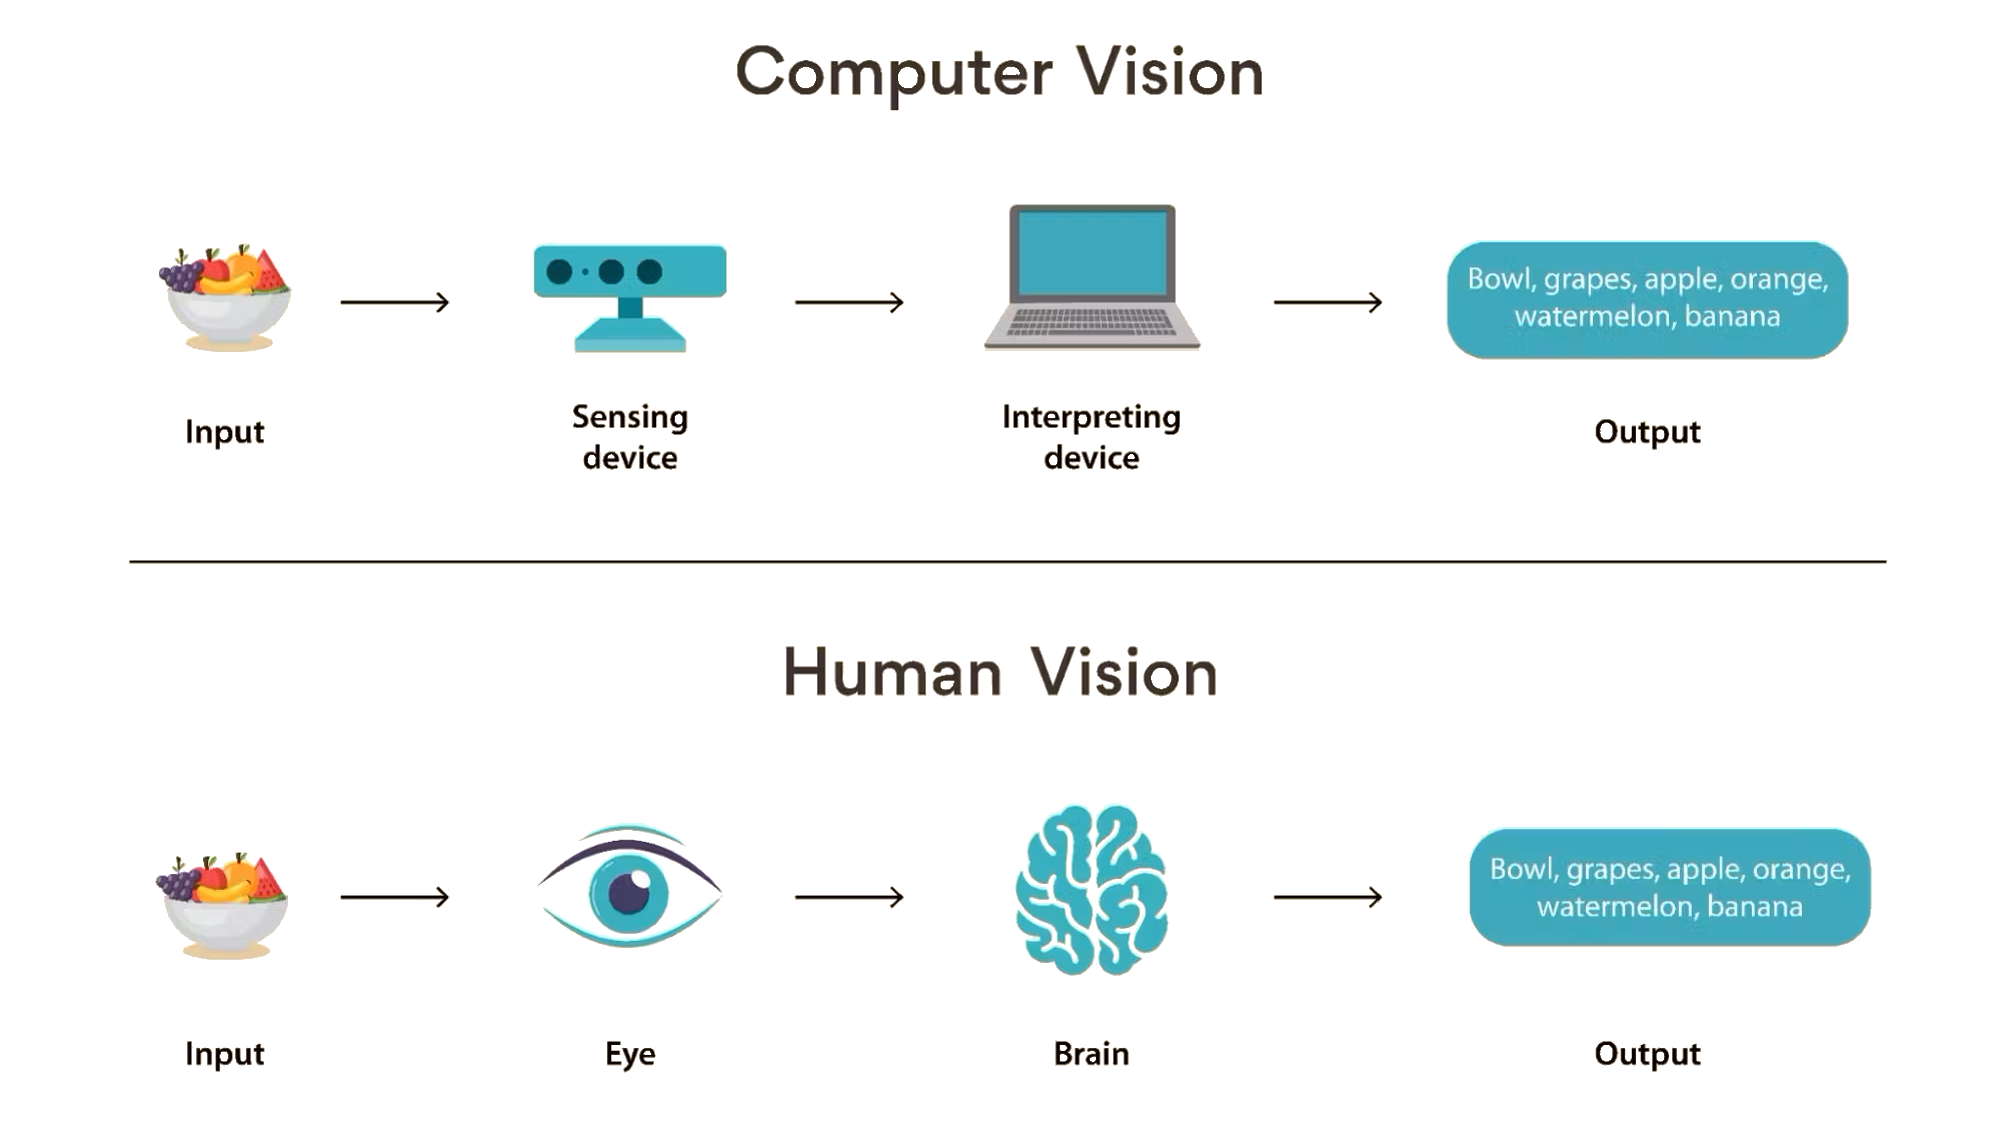
\includegraphics[width=0.85\linewidth]{figures/theory/machine-learning/computer-vision.png} \caption[Computer vision vs. human vision]{Comparison of computer vision and human vision, illustrating the similarities and differences in processing visual data \cite{turing:computer-vision}.} \label{fig:computer-vision} \end{figure}

\subsection{Artificial Neural Network}

One of the most influential technologies in modern \gls{ml} is the \gls{ann}. These networks excel at handling a wide range of data types, including images, audio, and text. Different neural network architectures are suited for specific tasks. For instance, \glspl{rnn}, especially those incorporating \gls{lstm}, are effective for sequential data such as text. \\

\newpage

In contrast, \glspl{cnn} are particularly effective in processing image data. Their architecture leverages convolutional layers to extract spatial features. \textbf{Spatial features} refer to patterns related to the position and arrangement of pixels in an image, making \glspl{cnn} highly efficient in image classification and object detection. An example of such a network applied to handwritten digit classification is shown in Figure~\ref{fig:convolutional-neural-network}.  \\

\begin{figure}[h!] \centering 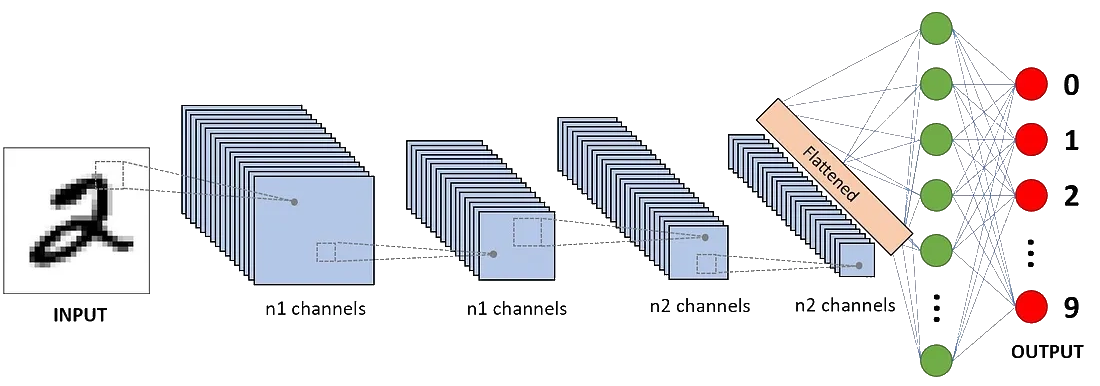
\includegraphics[width=0.75\linewidth]{figures/theory/machine-learning/convolutional-neural-network.png} \caption[CNN architecture for handwritten digit classification]{CNN architecture for classifying handwritten digits \cite{medium:cnn}.} \label{fig:convolutional-neural-network} \end{figure}

A key component of \glspl{cnn} is their ability to generate \textbf{feature maps}, which are the result of detecting spatial features at different locations in the image. These feature maps transform the input into a representation that highlights important visual patterns. As the image moves through the layers of the network, these feature maps capture crucial details such as edges, textures, and more complex shapes. Each feature map is the output of a convolutional layer, where filters are applied to extract relevant features. By emphasizing the most significant aspects of the image, these maps enable the network to learn and recognize patterns. This hierarchical approach to learning visual data has made \glspl{cnn} essential in a wide range of computer vision applications, from medical diagnostics to autonomous driving \cite{encord:cnn}. \\

\subsection{Supervised Learning}

Another fundamental concept in machine learning is supervised learning, where models are trained on labeled datasets. Each example in the dataset includes both an input and the correct output, allowing the model to learn how the input relates to the expected output. After training, the model can generalize this learned relationship to make predictions on new, unseen data \cite{geeksforgeeks:supervised-learning, google:supervised-learning}. \\

\subsection{Classification}

Within supervised learning, classification refers to predicting categorical outcomes. For example, a classification model trained on images of geometric shapes learns to associate visual features with specific shape categories. When shown a new image, the model attempts to determine the most likely category based on its prior learning. This process is illustrated in Figure~\ref{fig:supervised-learning}, which shows how labeled data is used to train a model to make accurate predictions on unseen inputs. \\

\begin{figure}[h!] 
    \centering 
    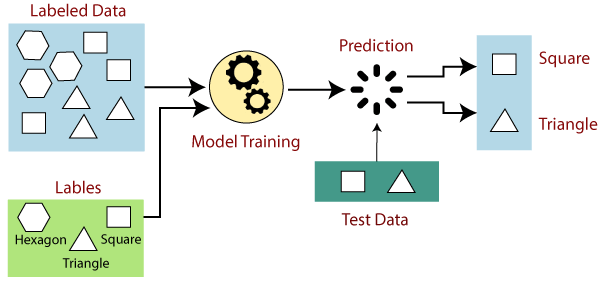
\includegraphics[width=0.75\linewidth]{figures/theory/machine-learning/supervised-learning.png} \caption[Supervised learning with labeled data]{Supervised learning process using labeled data for classification \cite{tpointtech:supervised-learning}.} 
    \label{fig:supervised-learning} 
\end{figure}

By combining supervised learning with powerful models such as \glspl{cnn}, machine learning systems have achieved remarkable success in tasks that require human-like perception and decision-making \cite{chengyi:cnn}. As these models become more accurate and versatile, deploying them efficiently to real-world applications becomes increasingly important.  \\

\subsection{Open Neural Network Exchange}

To facilitate deployment across diverse environments and platforms, \gls{onnx} provides an open-source format for representing machine learning models. It enables seamless transfer and interoperability between different frameworks, including TensorFlow and PyTorch. This open format allows developers to switch between different tools depending on their specific needs during training, deployment, or optimization \cite{roboflow:onnx}.\\

\subsection{Inference}

Once a model is trained, inference is the process of using the trained model to make predictions on new, unseen data. In the context of object detection, inference involves feeding an input image into the model, which processes the image and outputs predictions, usually in the form of object classes, bounding box coordinates, and confidence scores \cite{nvidia:inference}. \\

\newpage

\subsection{Model Performance}

After training and deploying a model, it is important to evaluate its performance. Two key metrics are precision and recall. \textbf{Precision} measures the proportion of correct positive predictions, indicating how many of the model’s positive predictions are actually correct. High precision means few false positives. \textbf{Recall} measures the proportion of actual positives detected by the model, showing how many relevant instances are identified. High recall means few false negatives \cite{builtin:precision-recall}.

\[
\text{Precision} = \frac{\text{True Positives}}{\text{True Positives} + \text{False Positives}}
\]

\[
\text{Recall} = \frac{\text{True Positives}}{\text{True Positives} + \text{False Negatives}}
\]

\section{Object Detection}
\label{sec:object-detection}

Object detection is a fundamental task in computer vision that involves both identifying and locating objects within an image. Unlike simple image classification, which only determines what objects are present, object detection also specifies where each object is by drawing a bounding box around it. This dual capability makes object detection essential for applications that require not just recognition, but also precise localization \cite{ibm:object-detection}. \\

\subsection{You Only Look Once}

\gls{leyolo} is a \gls{cnn}-based architecture designed for real-time object detection. It is a lightweight version of \gls{yolo} where its simplified architecture allows it to achieve faster inference times. This makes it particularly suitable for real-time applications, where quick detection is more important than achieving the highest possible accuracy. Like its predecessor, it divides an image into a grid, and each cell predicts whether an object is present, along with its bounding box coordinates \cite{openreview:leyolo}.\\

\subsection{Bounding Boxes}

Central to object detection is the use of bounding boxes. Bounding boxes are rectangular regions used to indicate the location of an object within an image. It is typically represented by four values: the center coordinates \((x_c, y_c)\), which define the center of the box, and the width \((w)\) and height \((h)\), which define the dimensions of the box. In object detection tasks, models predict these coordinates to both localize and classify objects within an image \cite{peopleforai:boundingbox}. An example of how bounding boxes are used to localize objects within an image is illustrated in Figure \ref{fig:boundingbox}.

\begin{figure}[h!]
    \centering
    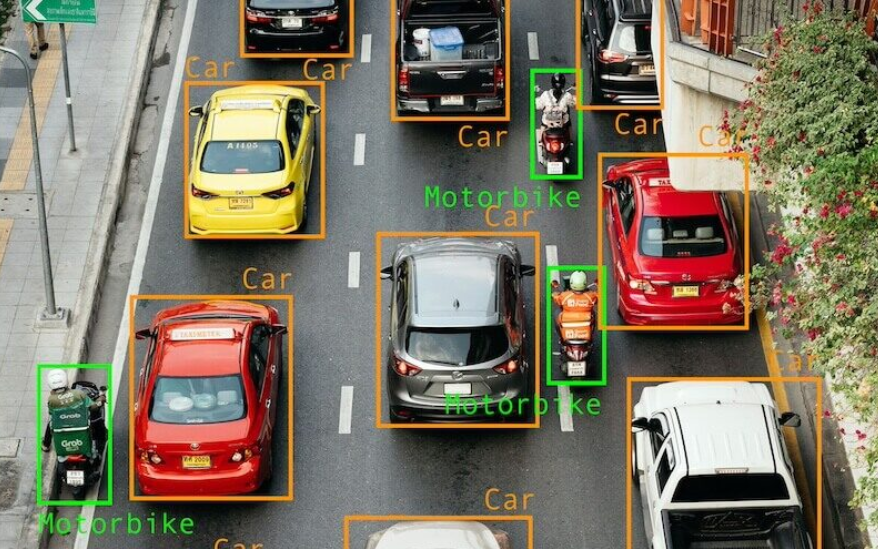
\includegraphics[width=0.60\linewidth]{figures/theory/image-recognition/bbox-example.png}
    \caption[Bounding box in object detection]{Example of a bounding boxes used in object detection to localize objects within an image \cite{peopleforai:boundingbox}.}
    \label{fig:boundingbox}
\end{figure}

\newpage

\subsection{Anchor Boxes}

To improve detection accuracy across different object sizes and shapes, models use anchor boxes. Anchor boxes are predefined bounding boxes of various sizes and aspect ratios, used as reference points for object detection. The sizes and aspect ratios of anchor boxes are determined by analyzing the object dimensions in the training dataset. The anchor boxes are placed over the feature map, which represents a transformed version of the input image. Rather than directly predicting bounding boxes, the model predicts offsets (shifts) relative to these anchor boxes, allowing it to adjust the box's position and size to fit the object. The model also predicts a confidence score indicating the likelihood that an object is present \cite{thinkautonomous:anchorboxes}. An illustration of how anchor boxes are positioned on the feature map is shown in Figure \ref{fig:anchor-box}.

\begin{figure}[h!]
    \centering
    
\includegraphics[width=0.56\linewidth]{figures/theory/image-recognition/anchor-boxes.png}
    \caption[Anchor boxes in object detection]{Illustration of anchor boxes on the feature map. These serve as initial reference boxes from which the model adjusts to better fit the actual objects in the image \cite{thinkautonomous:anchorboxes}.}
    \label{fig:anchor-box}
\end{figure}

\newpage

\subsection{Intersection Over Union}

To evaluate whether a predicted bounding box is accurate, a metric called \gls{iou} is used. \gls{iou} quantifies the overlap between the predicted bounding box and the ground truth box, the annotated box in the training dataset that precisely marks the object's true location. It is calculated as the ratio of the area of overlap to the area of union between the predicted and ground truth boxes:

\[
\text{IoU} = \frac{\text{Area of Overlap}}{\text{Area of Union}}
\]
An IoU value of 1.0 means a perfect match between the prediction and the ground truth, while 0 indicates no overlap. In practice, a prediction is considered correct if the IoU exceeds a certain threshold, commonly 0.5 \cite{ultralytics:iou}. \\

\subsection{Non Maximum Suppression}

 Once multiple bounding box predictions have been made, some of them may overlap. To handle this, a post-processing technique called \gls{nms} is used. \gls{nms} removes redundant or overlapping bounding boxes and keeps only the most confident prediction. It selects the bounding box with the highest confidence score and suppresses all other boxes that have a high \gls{iou} overlap with it. This process repeats iteratively until no overlapping boxes remain above the chosen IoU threshold. By applying \gls{nms}, object detectors produce cleaner and more accurate results, preventing multiple detections of the same object
\cite{thepythoncode:nms}. The effect of applying \gls{nms} is illustrated in Figure \ref{fig:nms}.

\begin{figure}[h!]
    \centering
    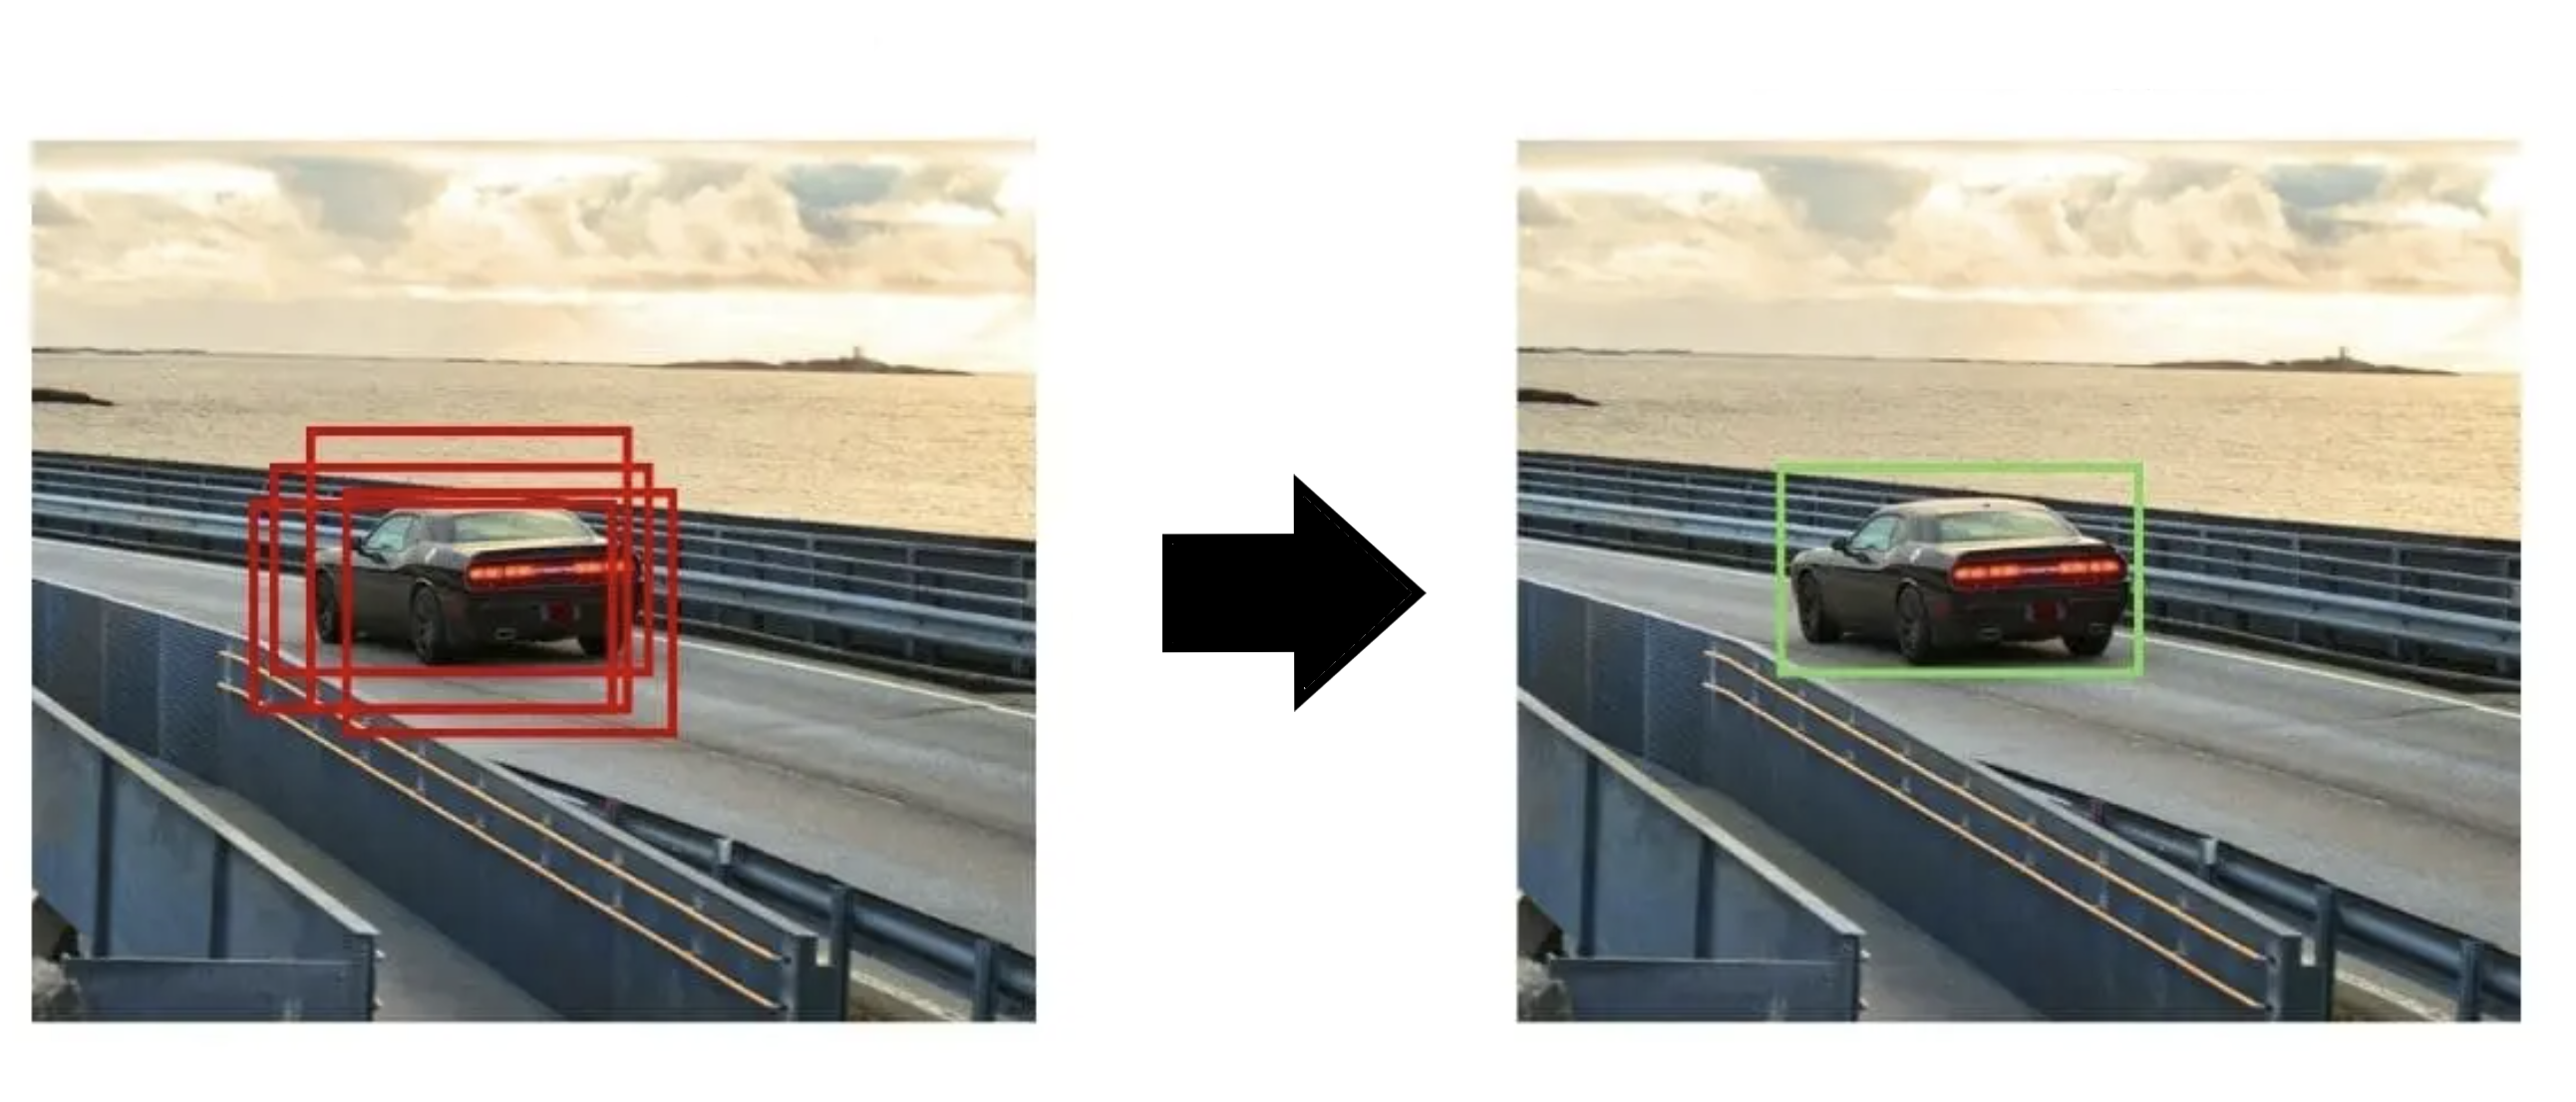
\includegraphics[width=0.75\linewidth]{figures/theory/image-recognition/nms.png}
    \caption[NMS before and after]{Illustration of NMS before and after its application \cite{thepythoncode:nms}.}
    \label{fig:nms}
\end{figure}

\newpage

\section{Geometric Methods in Image Processing}
\label{sec:geometric-methods}

\subsection{Normalization and Scaling}
\label{subsec:normalization-and-scaling}

Normalization in image processing involves adjusting pixel values to a consistent range, such as [0, 1] or [-1, 1]. This helps improve model performance by making the input data uniform. By adjusting pixel intensities from their original 0–255 range, normalization allows the model to process inputs more consistently, leading to faster and more stable convergence.
\textbf{Scaling} in image processing and machine learning involves resizing images to the format required by the model, as shown in Figure \ref{fig:scaling} \cite{brownlee:normalization}. 

\begin{figure}[h!]
    \centering
    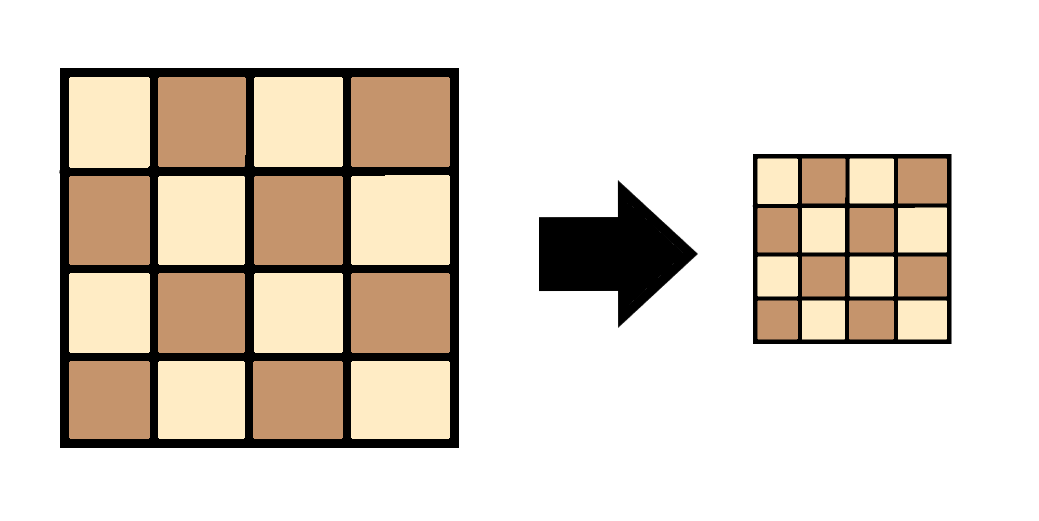
\includegraphics[width=0.75\linewidth]{figures/theory/image-recognition/scaling.png}
    \caption[Scaling before and after]{Illustration of the scaling process in image preprocessing, resizing the image to prepare it for model input.}
    \label{fig:scaling}
\end{figure}

\subsection{Perspective Transformation}
\label{subsec:perspective-transformation}

When an image is taken from a tilted viewpoint, objects that are normally rectangular, such as chessboards, appear distorted and no longer have right angles. A perspective transformation is a specific type of image warping that corrects distortions caused by viewing a flat object from an angle. A perspective transformation uses mathematical techniques to map points from the distorted image back to their correct, undistorted positions, as illustrated in Figure~\ref{fig:perspective-transformation} \cite{nvidia:perspective-transform}.

\begin{figure}[h!]
    \centering
    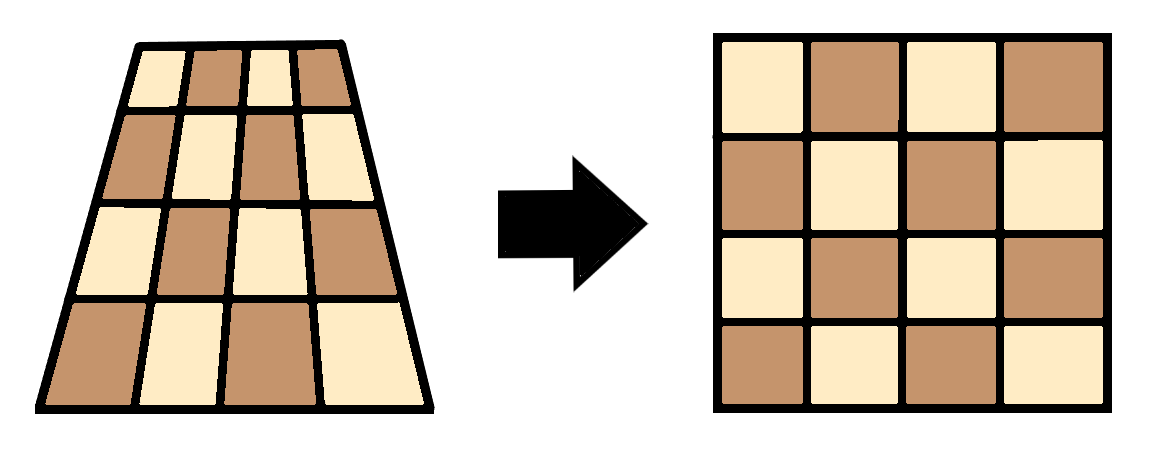
\includegraphics[width=0.75\linewidth]{figures/theory/image-recognition/perspective-transformation.png}
    \caption[Perspective transformation before and after]{Effect of perspective transformation on a distorted image. The algorithm corrects the distortion caused by an angled viewpoint, restoring the object’s original rectangular shape.}
    \label{fig:perspective-transformation}
\end{figure}

\subsection{Euclidean Distance}
\label{subsec:euclidean-distance}

The Euclidean distance is the straight-line distance between two points in a plane. For two points with coordinates \( \mathbf{p} = (p_1, p_2) \) and \( \mathbf{q} = (q_1, q_2) \), the Euclidean distance is given by:

\[
d(\mathbf{p}, \mathbf{q}) = \sqrt{(p_1 - q_1)^2 + (p_2 - q_2)^2}
\]

This formula gives the length of the path connecting the two points. Euclidean distance is used to measure the relationship between object centers or detected positions within an image \cite{cohen:precalculus}.

\subsection{Delaunay Triangulation}
\label{subsec:delaunay-triangulation}

Delaunay triangulation is a method of dividing a set of points into triangles such that no point is inside the circumcircle of any triangle. The circumcircle is the circle that passes through all three vertices of a triangle. It ensures that the triangles formed are as equiangular as possible,  meaning the triangle angles are close in size, minimizing the possibility of long, thin triangles. This property makes Delaunay triangulation particularly useful for applications involving geometric data, such as finding quadrilaterals from a set of points \cite{ianthehenry:delaunay}.

\section{Web}
\label{sec:web}

\subsection{Client-Server Architecture}
\label{subsec:client-server}

Client-server architecture is a network model in which multiple clients request and receive services from a centralized server over a local network or the internet. Clients interact with the system through an application interface, while the server handles data processing. This architecture enables centralized control, scalability, and efficient resource management \cite{liquidweb:client-server}. See Figure~\ref{fig:client-server-architecture}.

\begin{figure}[h!]
    \centering
    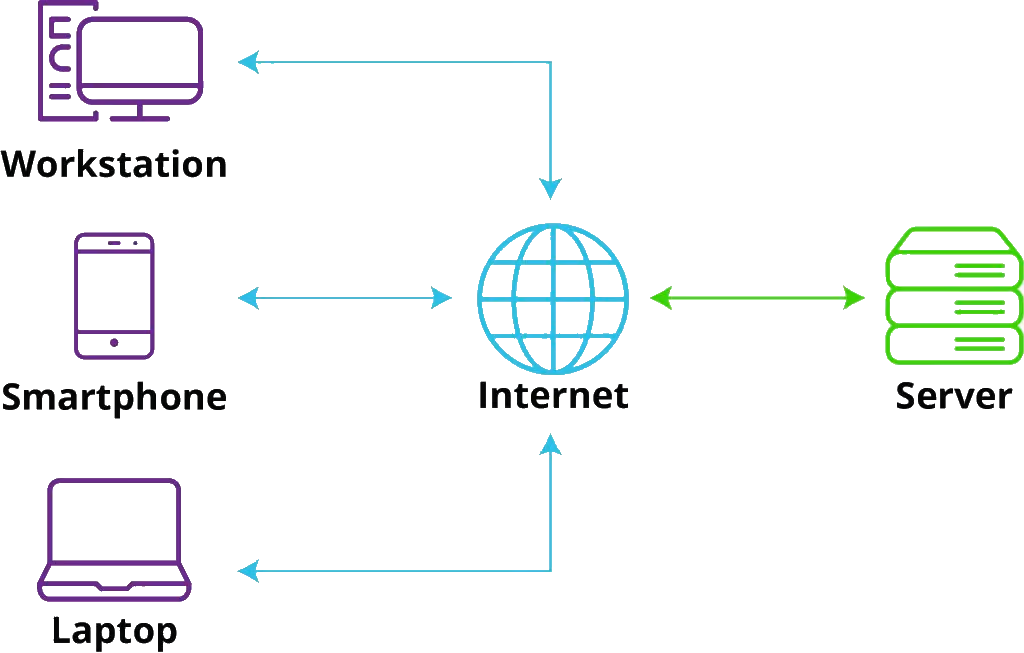
\includegraphics[width=0.75\linewidth]{figures/theory/client-server-architecture.png}
    \caption[Client-server architecture]{Client-server model where clients access services from a centralized server via the internet \cite{liquidweb:client-server}.}
    \label{fig:client-server-architecture}
\end{figure}

\subsection{REST}

\gls{rest} is an architectural style for designing networked applications, commonly implemented using \gls{rest}ful \glspl{api}. Unlike protocols such as WebSocket that maintain a persistent connection, \gls{rest} operates over the stateless \gls{http}, where each client-server interaction is independent. Clients initiate \gls{http} requests, such as \texttt{GET}, \texttt{POST}, \texttt{PUT}, or \texttt{DELETE}, to access or modify resources on the server, which responds with structured data, typically in JSON or XML format. This separation of concerns enhances scalability and modularity in web applications. \gls{rest} is widely used due to its simplicity, compatibility with web standards, and ease of integration. See Figure \ref{fig:rest-api-model} for an illustration of the \gls{rest} \gls{api} communication model \cite{medium:rest}.

\begin{figure}[h!]
\centering
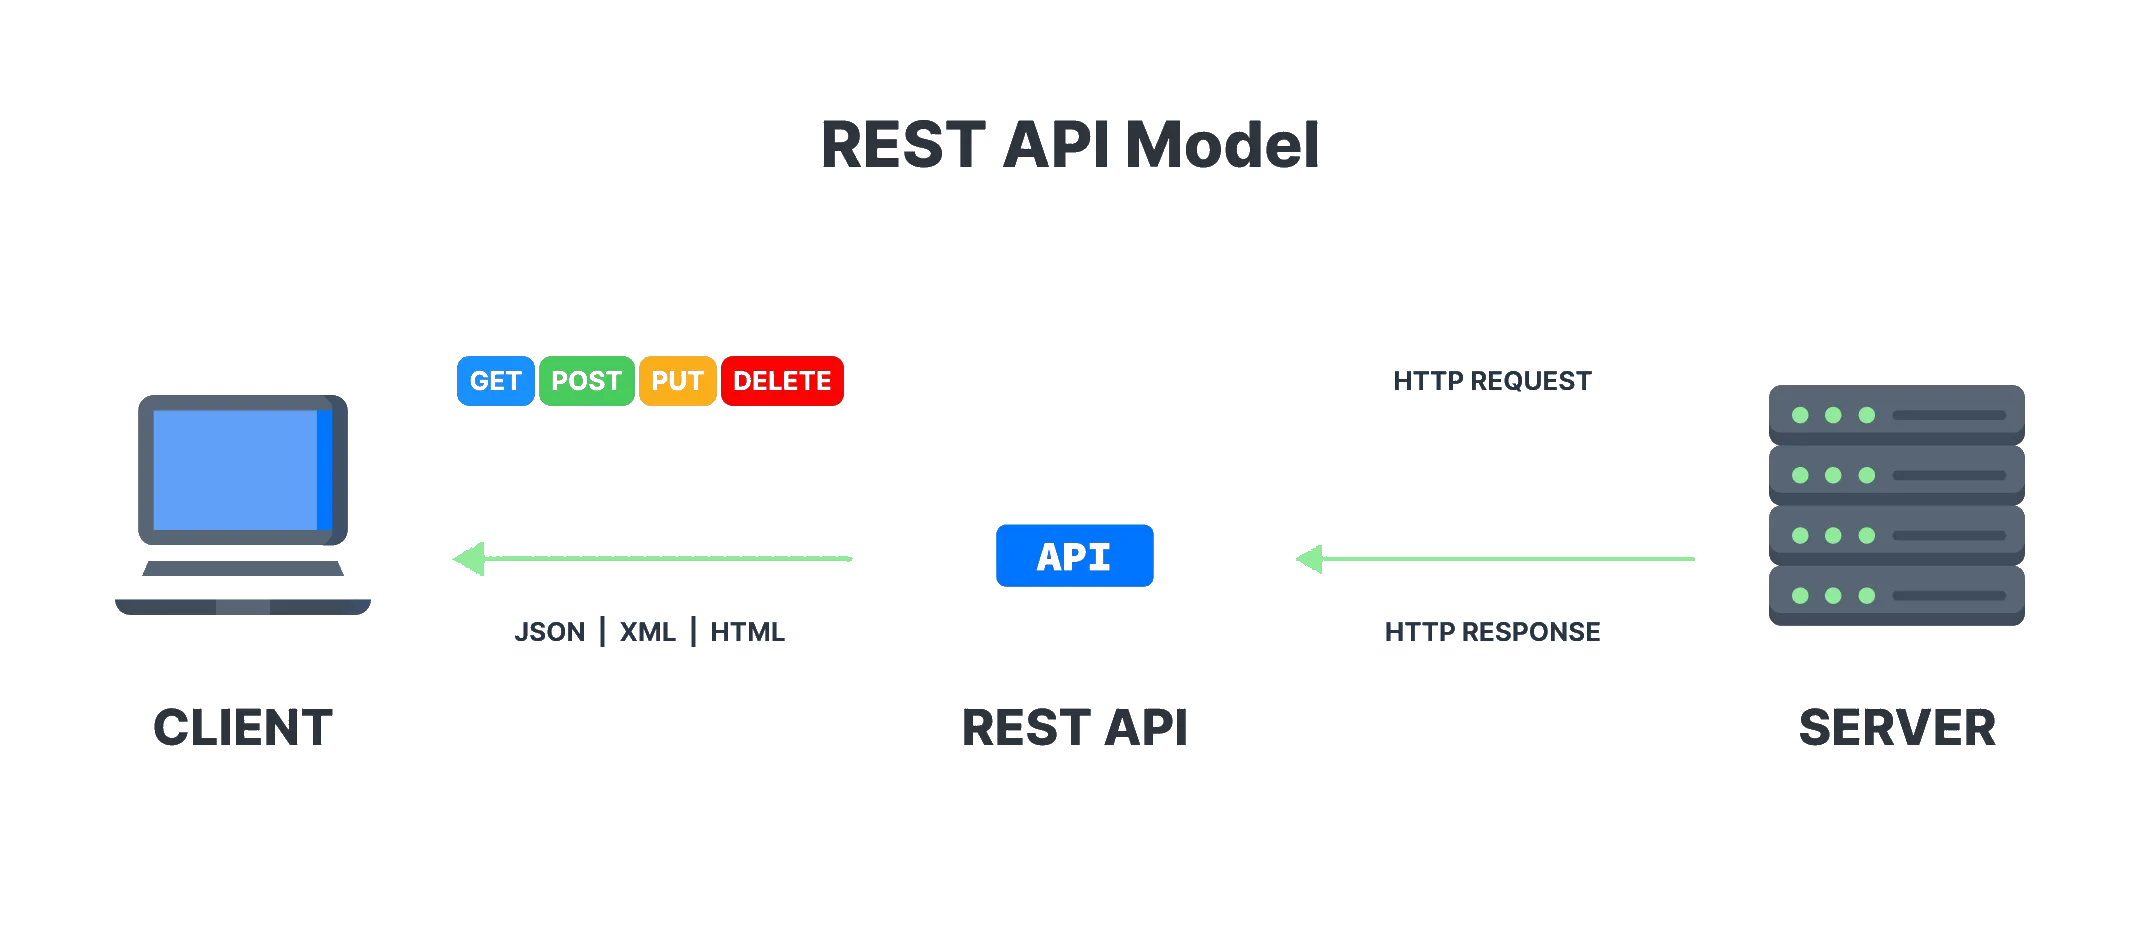
\includegraphics[width=0.95\linewidth]{figures/theory/rest.png}
\caption[REST API Model]{\gls{rest} \gls{api} Model}
\label{fig:rest-api-model}
\end{figure}

\subsection{WebSocket}
\label{subsec:websocket}

WebSocket is a standardized communication protocol that enables full-duplex communication over a single \gls{tcp} connection, making it well-suited for real-time web applications. Unlike traditional \gls{http} requests which follow a request-response model, WebSocket establishes a persistent connection that allows both the client and server to send and receive data at any time. This reduces the need for polling or long polling, lowering network traffic and latency. As a result, WebSocket improves the efficiency and responsiveness of data transmission, particularly in applications such as live data feeds and online games. See Figure \ref{fig:websocket-vs-http} for a comparison \cite{nodejs:websocket, apidog:websocket}.

\begin{figure}[h!]
    \centering
    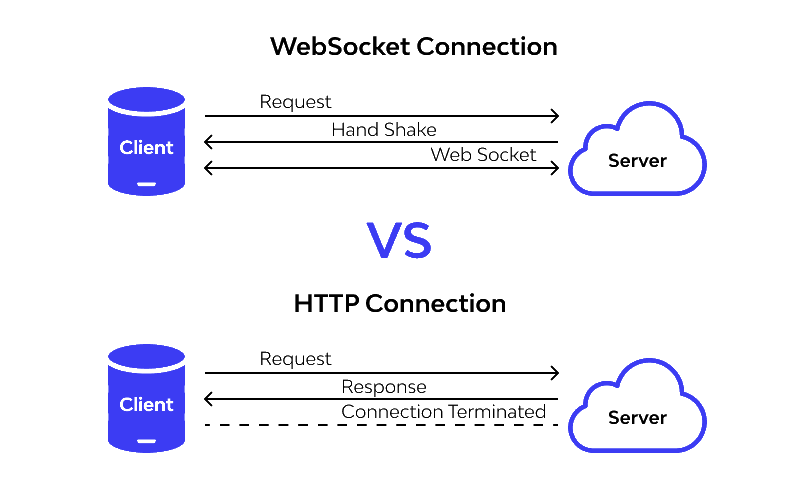
\includegraphics[width=0.8\linewidth]{figures/theory/websocket-vs-http.png}
    \caption[WebSocket connection vs. HTTP connection]{WebSocket connection vs. \gls{http} connection \cite{apidog:websocket}}
    \label{fig:websocket-vs-http}
\end{figure}

\newpage

\section{Design}
\label{sec:design}

Design is a fundamental aspect of creating digital products, focusing on how users interact with and experience technology. It encompasses various disciplines, including interaction design, which aims to make digital interfaces intuitive and user-friendly. Concepts such as wireframes, accessibility, and the \gls{wcag} are often introduced to emphasize the importance of structure, usability, and universal access. \\

\subsection{Wireframes}

Wireframes are essential tools in the early stages of interface design. They act as simplified blueprints for websites and applications, allowing designers to plan the placement of elements such as buttons, text, and images. Wireframes enable teams to focus on layout, content structure, and user flow before any visual styling or branding is applied \cite{balsamiq:wireframe}. Separating form from function allows designers to prioritize usability and navigation before applying visual design. \\

\subsection{Accessibility}

Another essential element in design of digital solutions is accessibility. Universal design ensures that products are usable by as many people as possible, regardless of disabilities \cite{uutilsynet:universellutforming}. This involves considering users with visual, auditory, motor, or cognitive impairments from the beginning of the design process. By planning for accessibility early, designers not only meet legal and ethical standards, but also improve the overall user experience for everyone. Inclusive design benefits a wider audience and reduces the need for costly adaptations later in development. \\

\newpage

To support accessibility in practice, the \gls{wcag} offer a detailed framework of recommendations. Developed by the \gls{w3c}, \gls{wcag} outlines how to make digital content more perceivable, operable, understandable, and robust \cite{levelaccess:wcag}. These guidelines are used globally to ensure web services are accessible to users with disabilities. Applying these principles from the wireframe stage onward helps integrate accessibility throughout the design process.

\section{Project Management}
\label{sec:project-management}

\textbf{Agile} is a flexible, iterative approach to managing projects, especially in software development. It emphasizes collaboration, continuous customer feedback, and the ability to quickly adapt to changing requirements throughout the project lifecycle, as illustrated in Figure \ref{fig:agile-methodology}. Agile breaks work into small, manageable increments, enabling teams to deliver value continuously and respond effectively to new information or challenges. One of the most widely used agile frameworks is \textbf{\gls{scrum}}, which organizes work into short, repeatable cycles called sprints \cite{scrumguides:scrum}. \\

\textbf{Sprints} are short time periods, usually between two and four weeks. At the start of each sprint, a meeting is held to decide the goals and how to achieve them. The objective is to complete a working piece of the product by the end of the sprint. During the sprint, a short \textbf{daily \gls{scrum} meeting} is held each day to share progress and plan the next steps. At the end of the sprint, a \textbf{sprint review} is conducted to present the completed work and gather feedback. Additionally, a \textbf{sprint retrospective} is held to reflect on what went well, identify areas for improvement, and define actions to enhance the workflow for the next sprint. \\

\begin{figure}[h!]
    \centering
    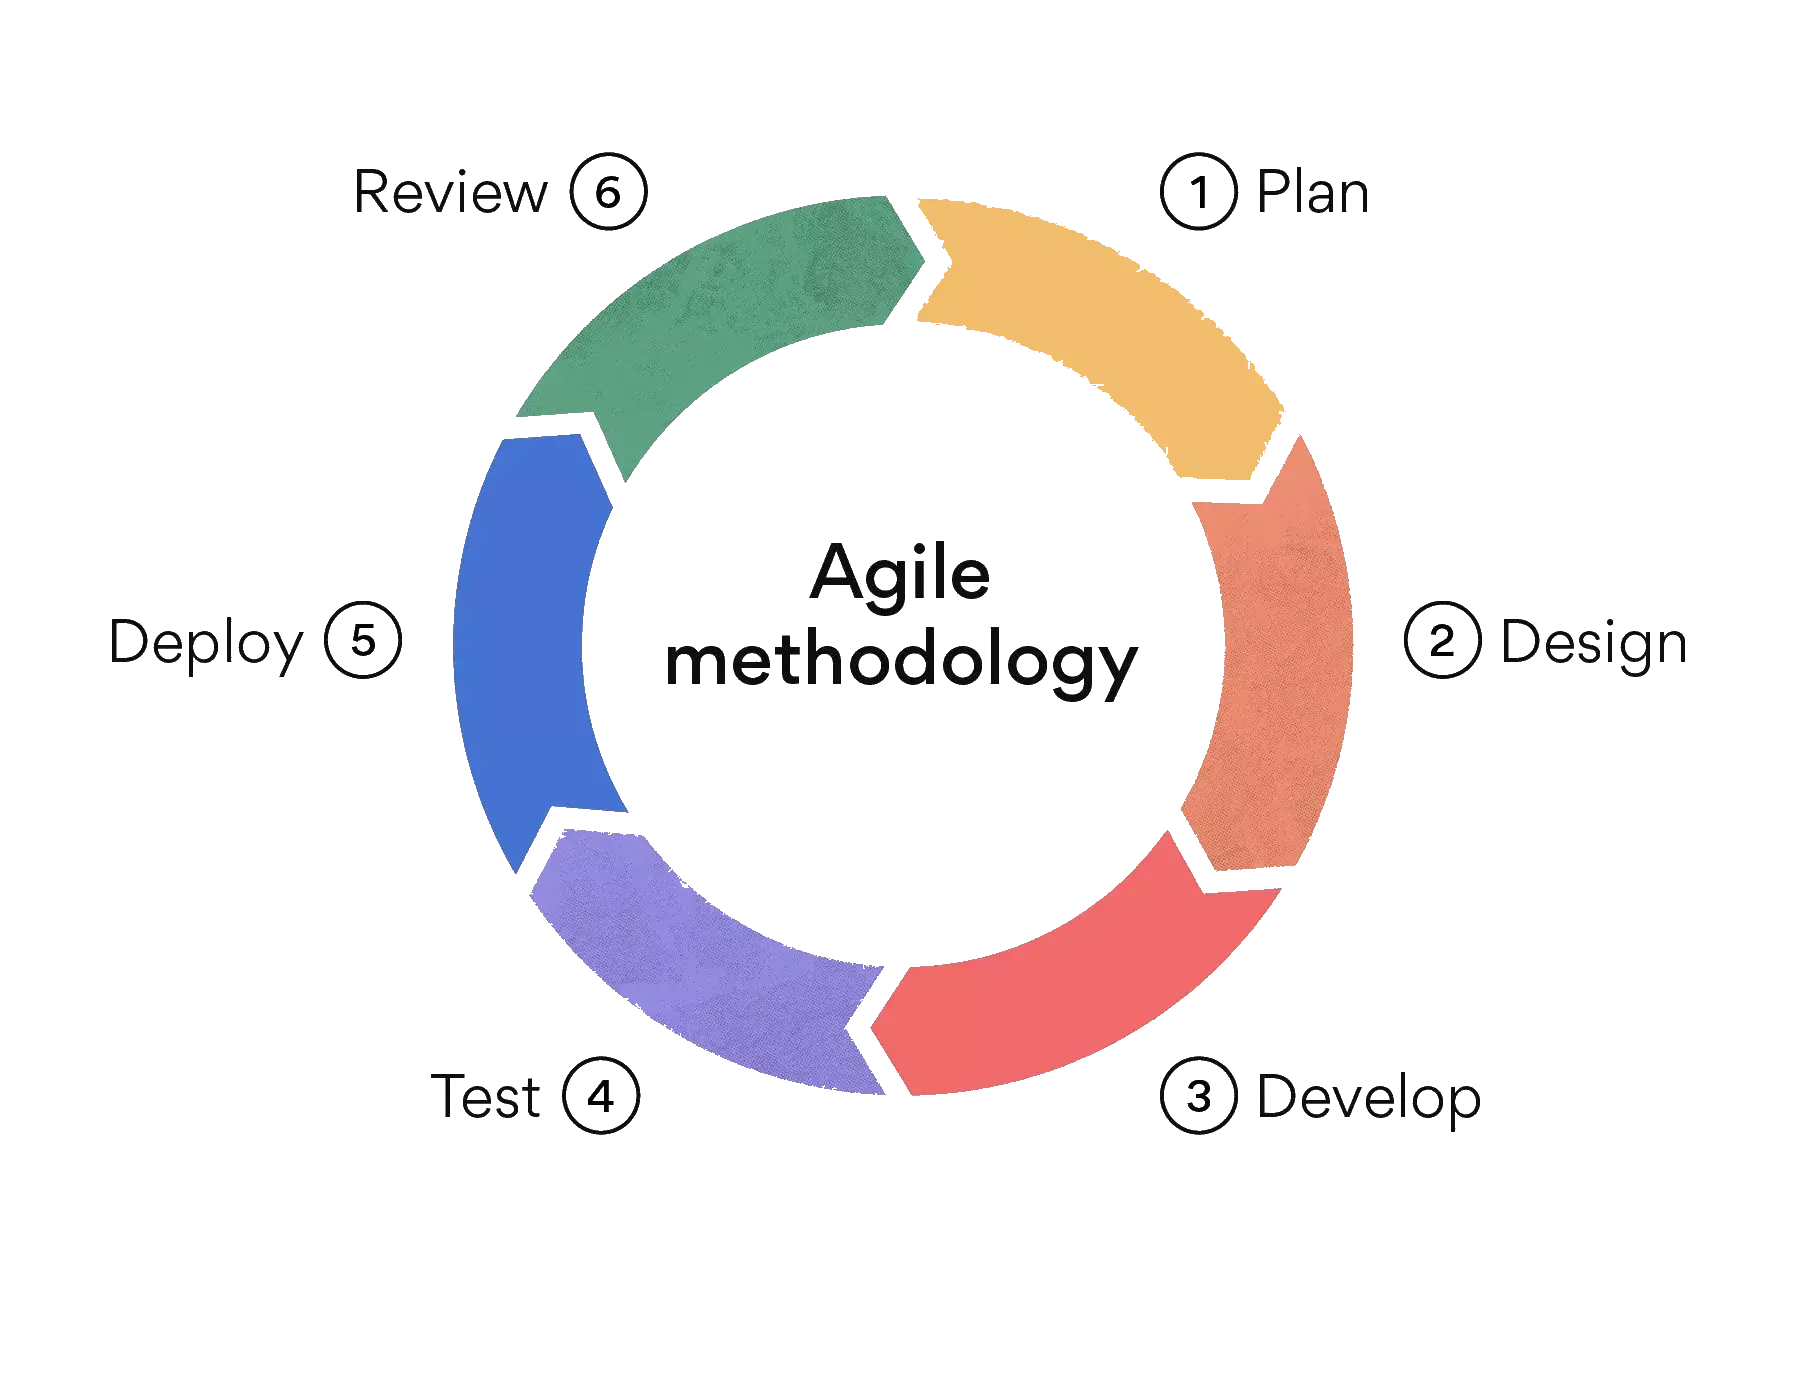
\includegraphics[width=0.75\linewidth]{figures/theory/agile-methodology.png}
    \caption{Agile Methodology}
    \label{fig:agile-methodology}
\end{figure}

\newpage

\gls{scrum} uses three main artifacts to organize and manage the work process. The \textit{product backlog} is a list of all features, enhancements, and fixes planned for the product. The \textit{sprint backlog} contains the specific tasks selected for implementation during the current sprint. Finally, the \textit{increment} is the completed, usable product delivered at the end of the sprint. Together, these artifacts promote transparency, align team efforts, and ensure consistent progress throughout the development cycle \cite{scrumguides:scrum}. \\

\gls{scrum} has three primary roles. The \textbf{product owner} is responsible for deciding what the team should work on and in what order. The \textbf{development team} builds the product and takes ownership of organizing and completing the work. The \textbf{\gls{scrum} master} facilitates the process by supporting the team, removing obstacles, and ensuring that \gls{scrum} practices are followed effectively.\\

% \newpage

\section{Software Engineering Principles}
\label{sec:software-engineering-principles}

\subsection{Code Review}
\label{subsec:code-review}

Code review is a process in which one or more developers examine another developer’s code before it is merged into a shared branch, such as the main branch. The purpose is to identify issues such as bugs, logic errors, or edge cases that may not have been caught during initial development \cite{gitlab:code-review}. \\

Modern version control systems often use pull requests to facilitate code reviews. A pull request is a formal proposal to merge changes from one branch into another and provides a platform for reviewing, discussing, and approving code. It also highlights differences between branches, helping reviewers understand and evaluate the proposed changes \cite{github:pr}.

\subsection{Cohesion and Coupling}
\label{subsec:cohesion-and-coupling}

\begin{quote}
\textit{"\textbf{Cohesion} refers to the degree to which elements within a module work together to fulfill a single, well-defined purpose. High cohesion means that elements are closely related and focused on a single purpose, while low cohesion means that elements are loosely related and serve multiple purposes"} \cite{geeksforgeeks:c&c}. \\
\end{quote}

\begin{quote}
\textit{"\textbf{Coupling} refers to the degree of interdependence between software modules. Tight coupling means that modules are closely connected and changes in one module may affect other modules. Loose coupling means that modules are independent, and changes in one module have little impact on other modules"} \cite{geeksforgeeks:c&c}. \\
\end{quote}

\begin{figure}[h!]
    \centering
    \subfloat{{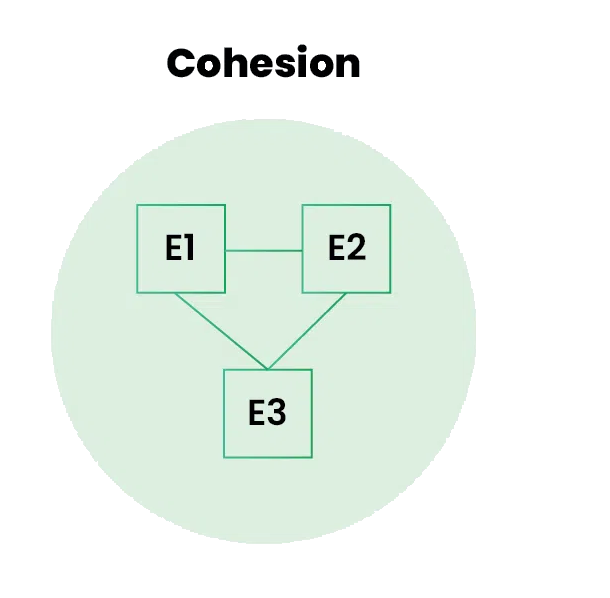
\includegraphics[width=0.4\linewidth]{figures/theory/cohesion.png}}}
    \subfloat{{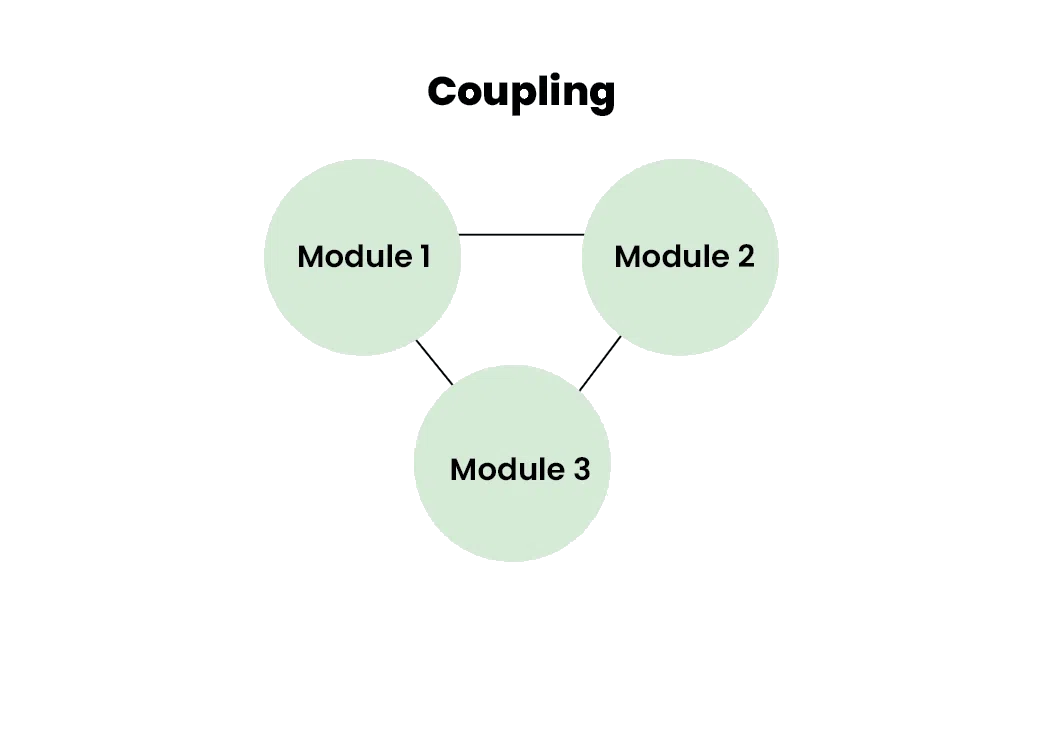
\includegraphics[width=0.4\linewidth]{figures/theory/coupling.png}}}

    \caption[Cohesion and coupling]{Cohesion shows internal module connectivity while coupling illustrates interdependence between modules \cite{geeksforgeeks:c&c}.}
    \label{fig:cohesion-coupling}
\end{figure}

\newpage

Cohesion and coupling impact the quality and maintainability of a system.
High cohesion and loose coupling are desirable, as they lead to systems that are easier to test, modify, and extend. This relationship is illustrated in Figure \ref{fig:cohesion-coupling} 
\cite{geeksforgeeks:c&c}.

\subsection{Documentation}
\label{subsec:documentation}

Documentation is an essential part of software development, providing written references for developers. It includes materials such as \gls{api} references, build instructions, user guides, and design specifications. Documentation supports understanding, maintenance, and helps preserve knowledge over time. It should be created and maintained alongside the code to stay accurate and useful throughout the project lifecycle \cite{geeksforgeeks:doc}.

\subsection{Software Testing}
\label{subsec:testing}

Software testing involves evaluating a system or its components to ensure they function correctly and meet user expectations. Two common approaches are unit testing and usability testing. \\

\subsubsection*{Unit Testing}

Unit testing focuses on verifying individual components of a software application, such as functions, methods, or classes in isolation. The goal is to confirm that each unit performs as intended under various conditions, improving reliability and simplifying debugging \cite{geeksforgeeks:unit-test}. \\

\subsubsection*{Usability Testing}

Usability testing, assesses the system from the end user’s perspective. It examines how easily users can navigate and interact with the interface to accomplish their goals. This process often involves observing users to identify confusion, inefficiencies, or obstacles in the user experience \cite{geeksforgeeks:user-test}. Both qualitative feedback and quantitative metrics are collected to evaluate effectiveness and satisfaction. The insights gained are then used to recommend improvements \cite{geeksforgeeks:user-test}.

\subsection{Type Safety}
\label{subsec:type-safety}

Type safety ensures that operations in a program are performed on the correct data types, helping catch errors early in development. In dynamically typed languages like JavaScript, lack of type enforcement can lead to hidden bugs. Enforcing type safety reduces runtime errors and improves code reliability \cite{dev:type-safety}.

\subsubsection*{Key Pillars of Type Safety}
\label{subsubsec:type-safety-pillars}

\begin{itemize}
\item \textbf{Reliability:} Enforcing correct data types prevents type-related runtime errors, improving application stability \cite{dev:type-safety}.

\item \textbf{Collaboration:} Clear type definitions make code easier to read and understand, aiding teamwork and maintainability \cite{dev:type-safety}.

\item \textbf{Efficient Debugging:} Detecting type errors early reduces debugging time and lowers the risk of runtime issues \cite{dev:type-safety}.
\end{itemize}

\cleardoublepage

\chapter{Methods}
\label{chp:methods}

\begin{center}
    \textit{This chapter outlines the development process, including the design and implementation of the application, tools and framework used, and testing strategies.}
\end{center}


\section{Machine Learning Models}
\label{sec:ml-models}

As mentioned in the theory chapter, ChessCam is an open-source tool for digitizing chess games using visual recognition. During the early development phase, this project was revisited in greater depth and ultimately chosen as the foundation for the \gls{ml} component. It employs two \glspl{cnn}, one for detecting chess pieces and another for locating the squares of the chessboard \cite{github:chesscam}. While the documentation was limited, the core logic and structure of the models were accessible in the repository. For any unclear aspects, communication with the developers helped ensure a correct understanding of the models. \\

The ChessCam repository offered models in multiple formats, including PyTorch and \gls{onnx}. To integrate them into the project, it was first necessary to understand the expected inputs and outputs. Netron was used to inspect and understand the models.


\subsection{Piece Detection Model}
The piece detection model was responsible for identifying and classifying chess pieces on the board. It expected \textbf{input} in the format \textbf{[1, 3, 288, 480]}. \textbf{1} represented the batch size, i.e. the number of images processed at once. \textbf{3} corresponded to the number of color channels (RGB), indicating that the image had to be in color. \textbf{288} and \textbf{480} denoted the height and width of the image in pixels, respectively. \\

The piece model output data in the format \textbf{[1, 16, 2835]}. \textbf{1} represented the batch size. \textbf{2835} represented the number of anchor boxes used in the detection and \textbf{16} consisted of two parts: \\

The first 4 values were offset values that adjusted the position and size of each anchor box to better align with a detected piece. These offsets were relative to the predefined anchor boxes, as illustrated in Table \ref{tab:piece-offset-table}.

\begin{table}[h]
    \centering
    \caption[Example offset values for anchor boxes, chess pieces]{Example offset coordinates for each anchor box with regard to identifying chess pieces.}  % Caption moved to top
    \renewcommand{\arraystretch}{1.3} % Increase row height to allow text to be on top
    \begin{tabular}{lcccc}
        \toprule
        \textbf{Anchor box} & \textbf{xcenter} & \textbf{ycenter} & \textbf{width} & \textbf{height} \\
        \midrule
        Anchor box 1 & -3.23 & 0.57 & -0.12 & -0.34 \\
        Anchor box 2 & 0.51 & -0.63 & 4.15 & 1.27 \\
        Anchor box 3 & 7.71 & 0.29 & -0.11 & 2.45 \\
        ... & ... & ... & ... & ... \\
        Anchor box 2835 & -0.04 & 2.11 & 1.15 & 5.32 \\
        \bottomrule
    \end{tabular}
    \label{tab:piece-offset-table}
\end{table}


The remaining 12 values represented the probabilities for each possible piece type after the offset value had been applied. With 12 different piece types, the model output 12 probabilities for each anchor box. The classification labels are shown in Table \ref{tab:piece-label-table}. Table \ref{tab:piece-probability-table} presents the predicted probabilities for each label across all anchor boxes. \\

% \vspace{2mm}

\begin{table}[ht]
\renewcommand{\arraystretch}{1.1}  % Increase row height slightly
\centering
\caption[Labels for chess piece types]{List of predefined class labels corresponding to the 12 chess piece types used for model classification.}
\begin{tabular}{|c|c|}
\hline
\multicolumn{2}{|c|}{\textbf{Model Labels}} \\  
\hline
\textbf{Black Pawn} & \textbf{White Pawn} \\
\textbf{Black Knight} & \textbf{White Knight} \\
\textbf{Black Bishop} & \textbf{White Bishop} \\
\textbf{Black Rook} & \textbf{White Rook} \\
\textbf{Black Queen} & \textbf{White Queen} \\
\textbf{Black King} & \textbf{White King} \\
\hline
\end{tabular}
\label{tab:piece-label-table}
\end{table}


\begin{table}[h]
    \centering
    \caption[Predicted chess piece after applying offset]{Predicted class probabilities for each anchor box after applying the offset.}  % Caption moved to top
    \renewcommand{\arraystretch}{1.3}
    \begin{tabular}{lcccc}
        \toprule
        \textbf{Anchor box} & \textbf{Black Pawn} & \textbf{White Pawn} & \textbf{Black Knight} & \textbf{...} \\
        \midrule
        Anchor box 1 & \raggedright 0.03 & \raggedright 0.71 & \raggedright 0.01 & ... \\
        Anchor box 2 & \raggedright 0.82 & \raggedright 0.02 & \raggedright 0.01 & ... \\
        Anchor box 3 & \raggedright 0.02 & \raggedright 0.01 & \raggedright 0.78 & ... \\
        ... & ... & ... & ... & ... \\
        Anchor box 2835 & \raggedright 0.01 & \raggedright 0.03 & \raggedright 0.05 & ... \\
        \bottomrule
    \end{tabular}
    \label{tab:piece-probability-table}
\end{table}

\newpage

There were 2835 predefined anchor boxes spread across the image, each serving as a candidate location for detecting a chess piece. During training, the model learned to adjust these anchor boxes to better match the actual pieces on the board. It achieved this by predicting 4 offset values that modified the location and size of each anchor box. At runtime, for each anchor box, the model used these learned offsets and output 12 class probabilities, indicating the likelihood of each chess piece type being present at that location.

\subsection{XCorners Detection Model}
The corner detection model identified the points where the edges of the inner squares on the chessboard met, referred to as \textit{intersection points} or \textit{xcorners}. Up to 49 intersection points could be detected in a single image. These points are illustrated in Figure \ref{fig:xcorners-chessboard}.

\begin{figure}[h!]
    \centering
    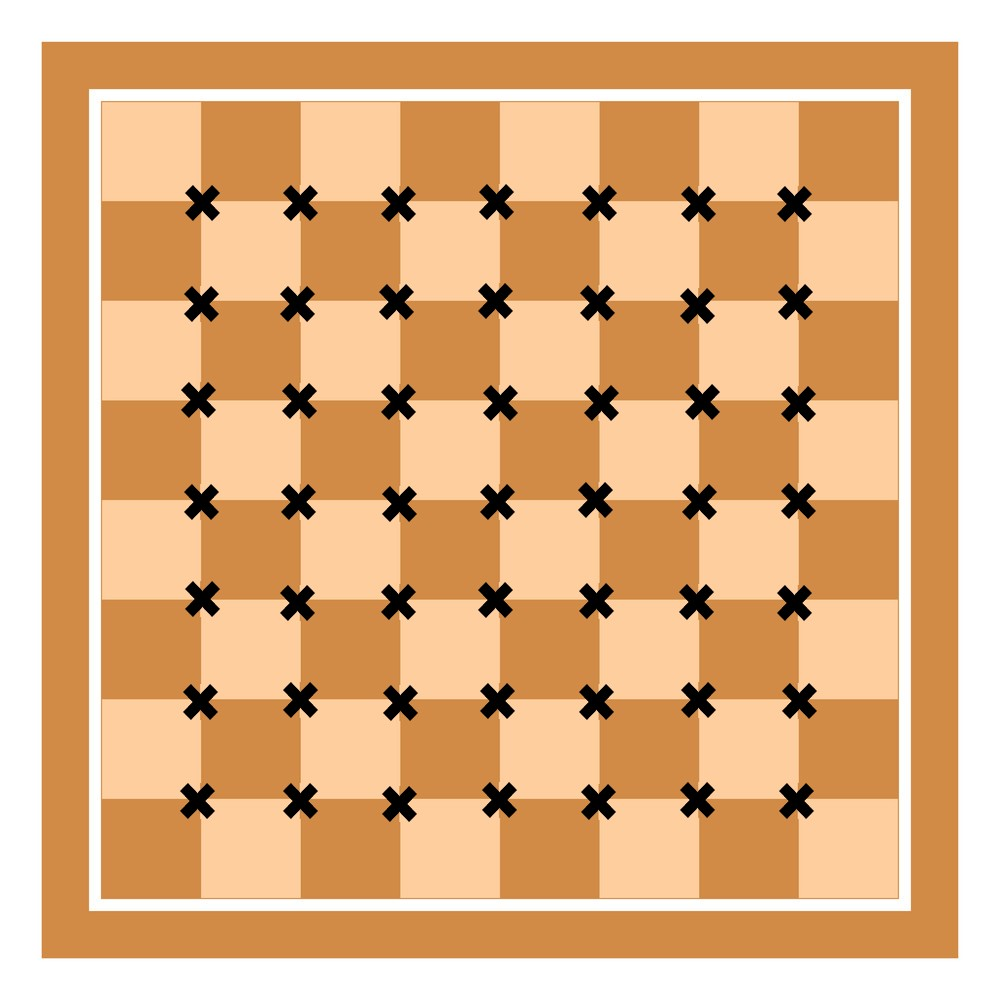
\includegraphics[width=0.75\linewidth]{figures/methods/ml-models/xcorners_chessboard.jpg}
    \caption[Detected intersection points on chessboard]{Visualization of intersection points where the edges of the inner squares on the chessboard meet. The model identified and predicted these points. Up to 49 intersection points could be detected in a single image \cite{vectorstock:chessboard-svg}.}
    \label{fig:xcorners-chessboard}
\end{figure}

The input for the corner model was the same as the piece model: \textbf{[1, 3, 288, 480]}. The corner model output predictions in the format \textbf{[1, 5, 2835]}. \textbf{1} represented the batch size. \textbf{2835} represented the number of anchor boxes used in the detection and \textbf{5} consisted of two parts: \\

\newpage

The first 4 values were offset values that adjusted the position and size of each anchor box, aligning it more accurately with a potential intersection point. These offsets were relative to the original anchor box coordinates, as shown in Table \ref{tab:corner-offset-table}.

% \newpage

\begin{table}[h]
    \centering
    \caption[Example offset values for anchor box, intersection points]{Example offset coordinates for each anchor box with regard to identifying intersection points.}  % Caption moved to top
    \renewcommand{\arraystretch}{1.3} % Increase row height to allow text to be on top
    \begin{tabular}{lcccc}
        \toprule
        \textbf{Anchor box} & \textbf{xcenter} & \textbf{ycenter} & \textbf{width} & \textbf{height} \\
        \midrule
        Anchor box 1 & -1.43 & 3.27 & -0.52 & -2.21 \\
        Anchor box 2 & 2.51 & -7.61 & 0.15 & 4.17 \\
        Anchor box 3 & -3.71 & 1.49 & -4.21 & 2.45 \\
        ... & ... & ... & ... & ... \\
        Anchor box 2835 & -2.04 & 3.29 & -0.35 & 1.24 \\
        \bottomrule
    \end{tabular}
    \label{tab:corner-offset-table}
\end{table}

The final value was the probability that the adjusted anchor box corresponded to an intersection point on the chessboard, as illustrated in Table~\ref{tab:corner-probability-table}. \\

\begin{table}[h]
    \centering
    \caption[Predicted intersection points after applying offset]{Predicted intersection probabilities for each anchor box after applying the offset.}
    \renewcommand{\arraystretch}{1.3}
    \begin{tabular}{lc}
        \toprule
        \textbf{Anchor Box} & \textbf{Intersection Probability} \\
        \midrule
        Anchor Box 1 & 0.06 \\
        Anchor Box 2 & 0.91 \\
        Anchor Box 3 & 0.03 \\
        ... & ... \\
        Anchor Box 2835 & 0.87 \\
        \bottomrule
    \end{tabular}
    \label{tab:corner-probability-table}
\end{table}


% \newpage


\subsection{Combining The Models}

To track chess piece movements, the process began with identifying the individual squares of the chessboard. Achieving this required first determining the outer corners of the board, which served as reference points for constructing the grid. Once the corners were located, the chessboard could be subdivided into an 8×8 grid of uniformly sized squares. Given the known distances between the corners and the regular structure of the board, the center point of each square could be accurately calculated. These center points were then used as the basis for mapping each detected piece to a specific square, as illustrated in Figure~\ref{fig:chessboard-centers}.

\newpage



\begin{figure}[h!]
    \centering
    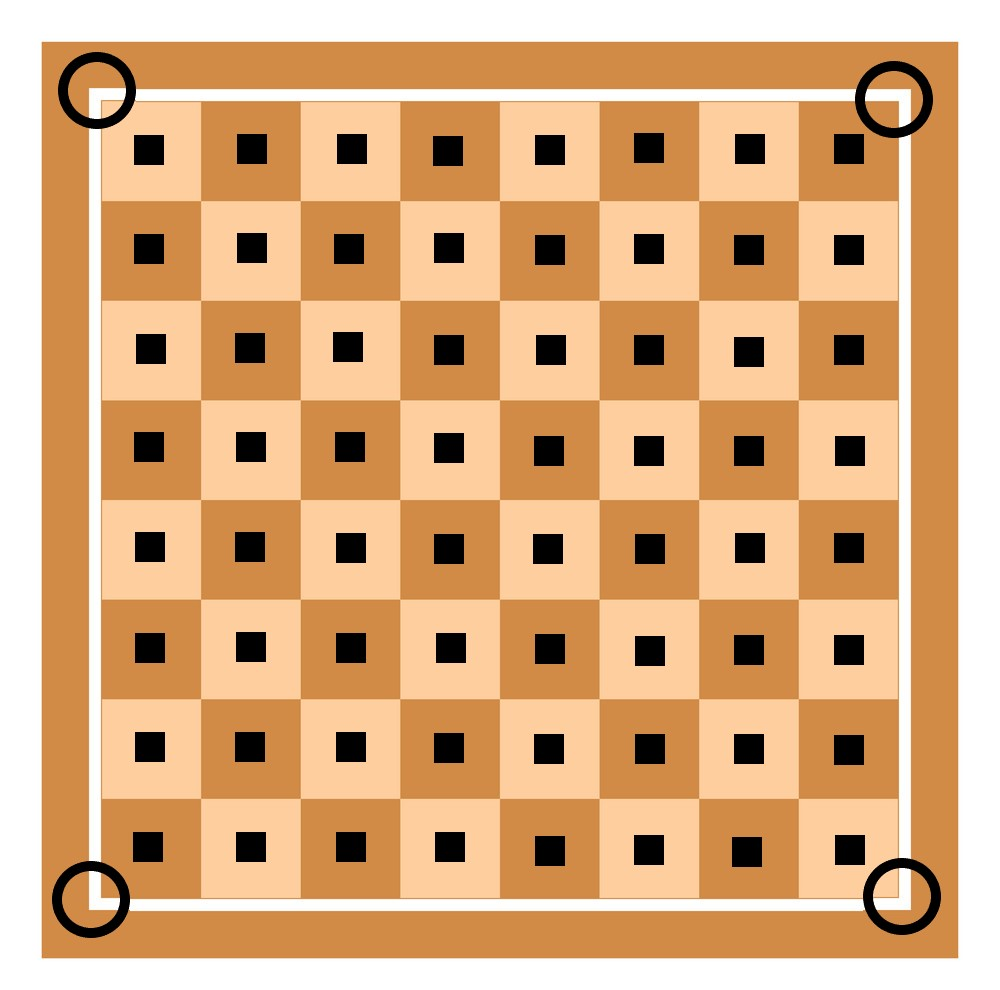
\includegraphics[width=0.75\linewidth]{figures/methods/ml-models/outer_corners_centers_chessboard.jpg}
    \caption[Chessboard corners and centers]{Visualization of the corners of the chessboard and the centers of each individual square \cite{vectorstock:chessboard-svg}.}
    \label{fig:chessboard-centers}
\end{figure}


The bottom center of each piece’s bounding box was selected as its representative location, as highlighted in Figure~\ref{fig:bbox-black-pawn}. Each detected piece was then mapped to the nearest square center based on the minimum Euclidean distance, as described in Section \ref{subsec:euclidean-distance}. This approach made it possible to accurately assign each piece to a specific square on the chessboard.


% \newpage


\begin{figure}[h!]
    \centering
    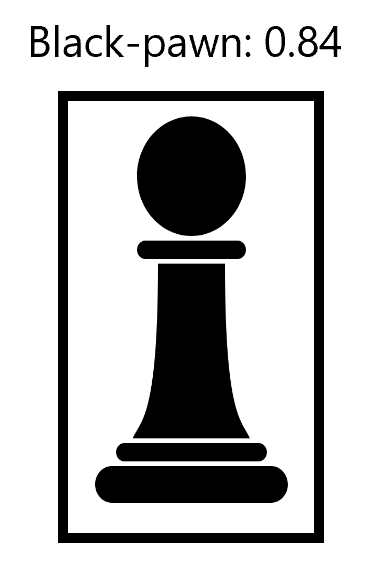
\includegraphics[width=0.25\linewidth]{figures/methods/ml-models/black-pawn.png}
    \caption[Detected chess piece and its bounding box]{Example of a detected chess piece with its classification confidence score. The bottom center of the bounding box was used as the reference point for mapping the piece to its corresponding square \cite{svgrepo:black-pawn-svg}.}
    \label{fig:bbox-black-pawn}
\end{figure}


\subsubsection*{Board Detection}

Each frame captured by the camera was processed by the two models. Before inference, the frame had to match the models’ expected input dimensions [1, 3, 288, 480]. This process included scaling the frame, normalizing the pixel values to fall within the range [0, 1], and converting the image to the appropriate data type. \\

After inference, the models produced the prediction outputs: [1, 16, 2835] for pieces and [1, 5, 2835] for intersection points. To identify the most reliable predictions, low-confidence entries were first filtered out. Furthermore, \gls{nms} was applied to further refine the results. This process ensured only the most accurate locations for the pieces and intersections were retained. \\

To identify the board corners of the chessboard, Delaunay triangulation was used, as described in Section \ref{subsec:delaunay-triangulation}. Delaunay triangulation was applied to the intersection points to generate a set of candidate triangles. By iterating over these triangles and examining their shared vertices, the algorithm identified potential quadrilaterals (four-sided shapes) that represented the four corners of the chessboard. Once a list of candidate quadrilaterals was generated, each was scored based on how well it fit the original intersection points. The quadrilateral with the highest score was then selected as the most likely representation of the board corners. \\

With the corners identified, the next step was to correct the distortion caused by the camera angle. When viewed at an angle, the board appeared skewed due to varying distances between the camera and different parts of the board. This distortion was corrected by using a perspective transformation. Specifically, the inverse of the transformation matrix responsible for the distortion was computed. By applying this inverse to the distorted image, the transformation that warped the image was reversed, effectively 'flattening' the distorted chessboard back to its ideal, top-down view. Once the inverse matrix was applied, the resulting coordinates provided the corrected positions of the corners in the distorted image. \\

With the distortion corrected, the board was treated as an 8×8 grid of uniformly sized squares, each occupying a unit-length cell. The center of each square lies midway between its edges, resulting in center coordinates that ranged from 0.5 to 7.5 in both the x and y axes. The center of the first square was at (0.5, 0.5), the second at (1.5, 0.5), and so on up to (7.5, 7.5). \\

To finalize the board orientation, the average center of all black and white pieces was computed. The board was then rotated in four 90-degree increments. For each rotation, the midpoints of the expected white and black sides were calculated as the average coordinates between pairs of corners. Specifically, the midpoint for the white side was calculated between ‘a1’ and ‘h1’, and for the black side between ‘a8’ and ‘h8’. The rotation that minimized the distance between piece centers and these midpoints was selected as the correct alignment. Based on this orientation, the labels ‘a1’, ‘h1’, ‘a8’, and ‘h8’ were assigned to the corners of the chessboard. A visualization of this process is shown in Figure \ref{fig:board_label_assignment}.

\begin{figure}[h!]
\centering
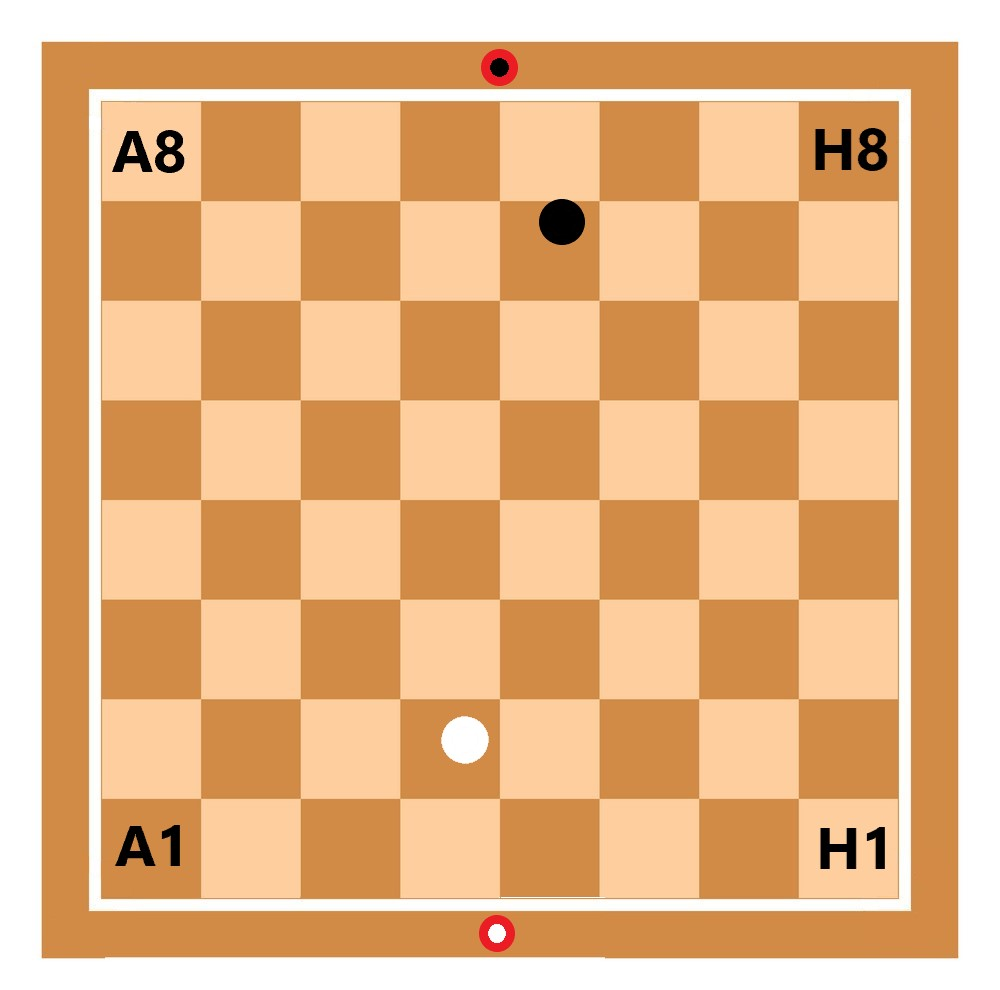
\includegraphics[width=0.70\linewidth]{figures/methods/ml-models/label_assignment_board.jpg}
\caption[Assigning labels to chessboard]{The white and black circles represent the average centers of the white and black pieces. The red circles indicate the midpoints between the corners on the white and black sides  \cite{vectorstock:chessboard-svg}.}
\label{fig:board_label_assignment}
\end{figure}



\subsubsection*{Move detection}

After detecting the chessboard and pieces, the application continuously processed each incoming video frame to determine whether a move had occurred. For every frame, the internal board state was updated based on the observed positions of the chess pieces. \\

To ensure stability, the system used a decay-based mechanism that blended the current detections with the previous state. This approach helped smooth out transient errors caused by occlusions or momentary inconsistencies in the video feed. Additionally, updates were throttled to fixed intervals, reducing computational overhead and avoiding unnecessary changes due to minor fluctuations in detection. \\

Once the updated board configuration was determined, it was compared to the set of legal moves for the current state. If a high-confidence legal move was identified, it was registered and applied. The move was then committed to the internal board state and sent to the frontend via the WebSocket connection to support ongoing analysis and visualization.

\newpage

\subsubsection*{Pre-recorded video}

To streamline the development of the \gls{ml} model, prerecorded video footage was used instead of a live camera feed. This approach provided a consistent and controlled environment where the model could be developed and refined by replaying the same chess game repeatedly. Using static video eliminated the need to physically set up the chessboard and camera for each iteration, significantly speeding up the development process. \\

\begin{figure}[h!]
    \centering
    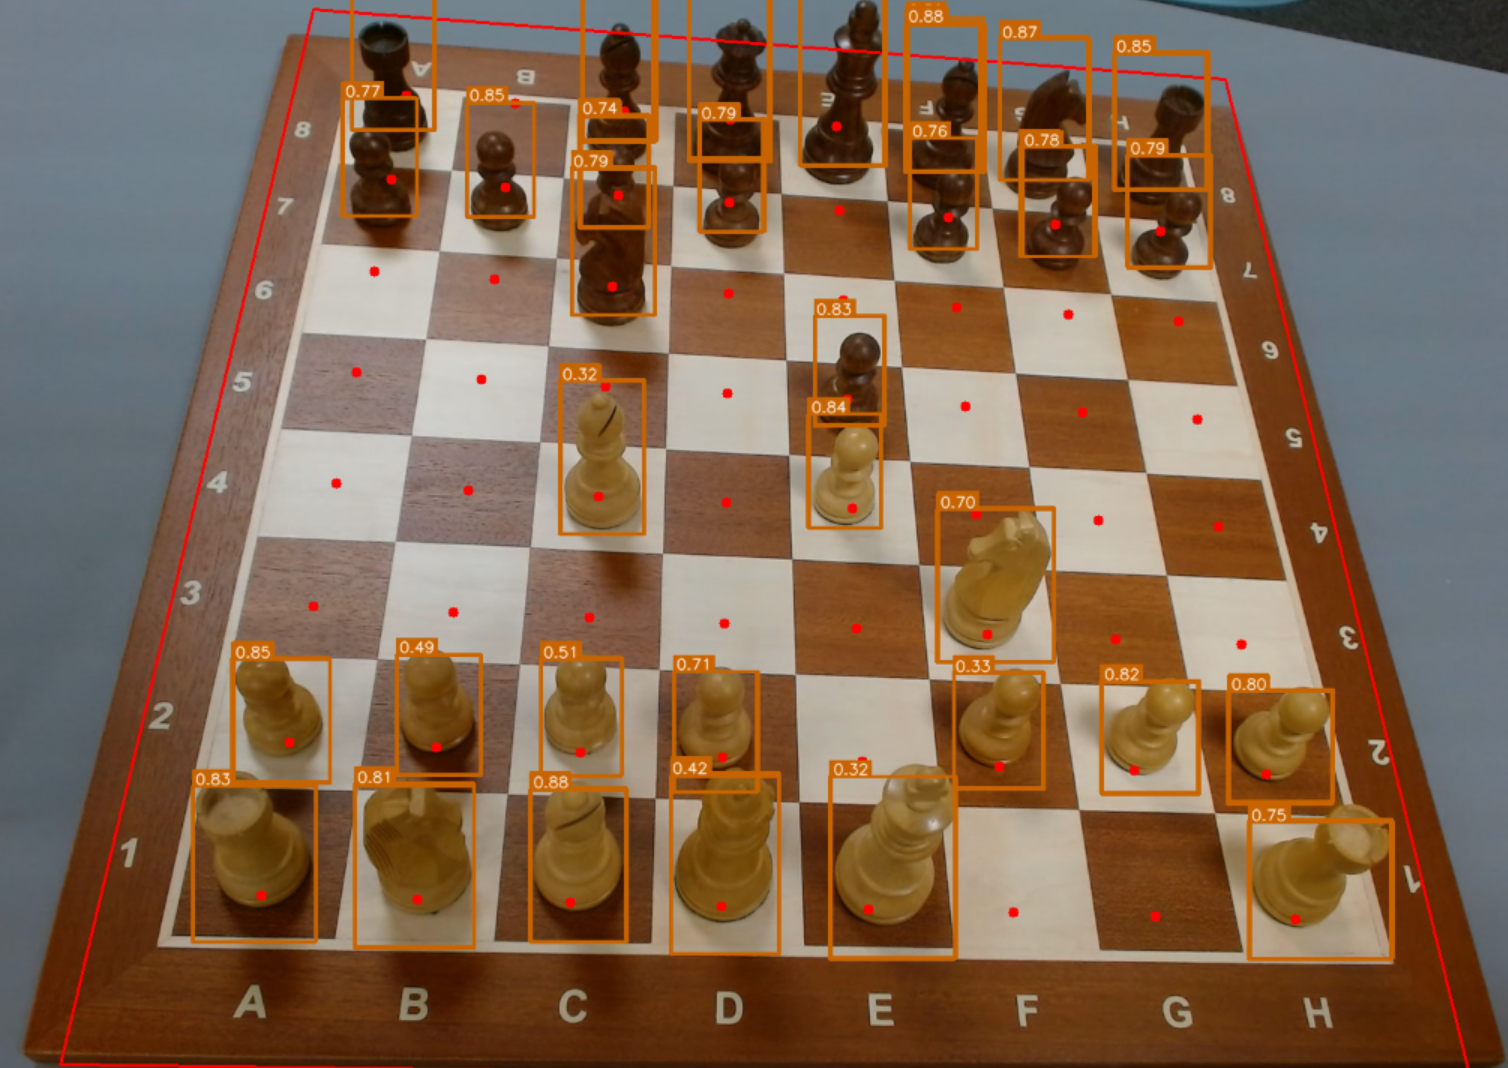
\includegraphics[width=0.75\linewidth]{figures/methods/ml-models/piece-model.png}
    \caption[Visualization of piece model and corner model]{Visualization of the detected pieces and centers of the squares.}
    \label{fig:websocket-vs-http}
\end{figure}

\section{Design}
\label{subsec:wireframe}

\subsubsection*{Control Panel}

The Control Panel is a desktop interface for tournament organizers to manage the digitization of multiple physical chessboards. The interface is minimal and task-focused, enabling efficient system setup and management with little technical effort. It follows a simple three-step workflow:

\begin{enumerate}
\item \textbf{Select number of cameras:} Specify how many cameras are connected. This determines how many boards will be monitored  (Figure \ref{fig:control-panel-1}).
\item \textbf{Start cameras and digitization:} Starts the camera feeds, board state recognition, and move validation (Figure \ref{fig:control-panel-2}).
\item \textbf{Restart boards for new round:} Resets all boards at the end of a round, preparing the system for the next games (Figure \ref{fig:control-panel-3}).
\end{enumerate}

\newpage

\begin{figure}[h!]
    \centering
    \begin{subfigure}[h!]{0.40\linewidth}
        \centering
        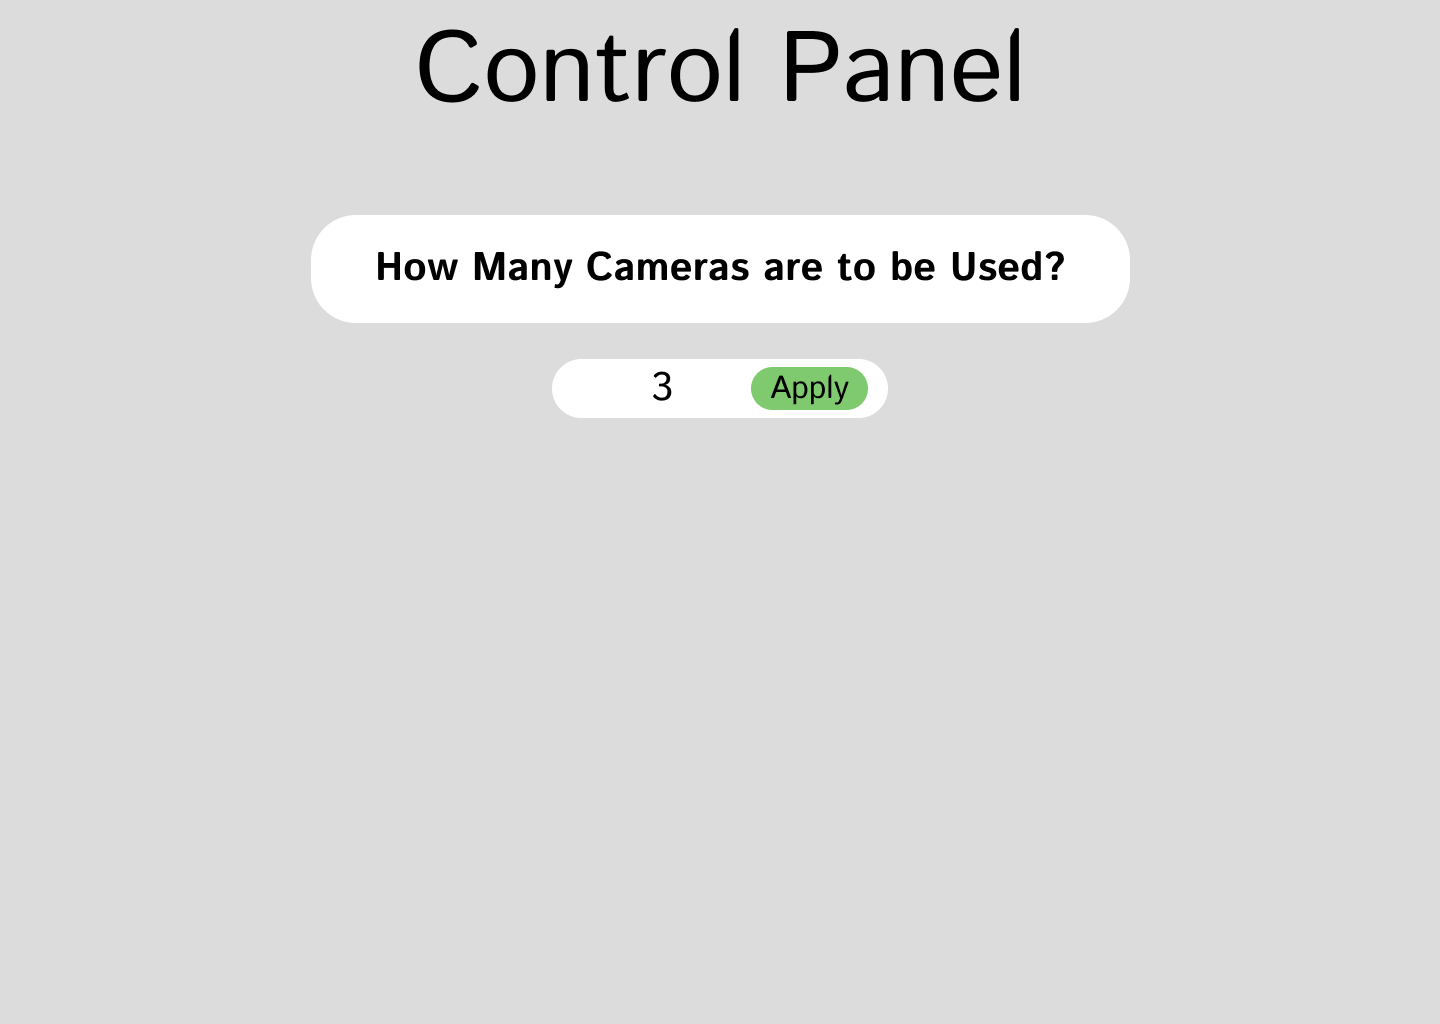
\includegraphics[width=\linewidth]{figures/methods/wireframes/control-panel-1.png}
        \caption{Step 1}
        \label{fig:control-panel-1}
    \end{subfigure}
    \hfill
    \begin{subfigure}[h!]{0.40\linewidth}
        \centering
        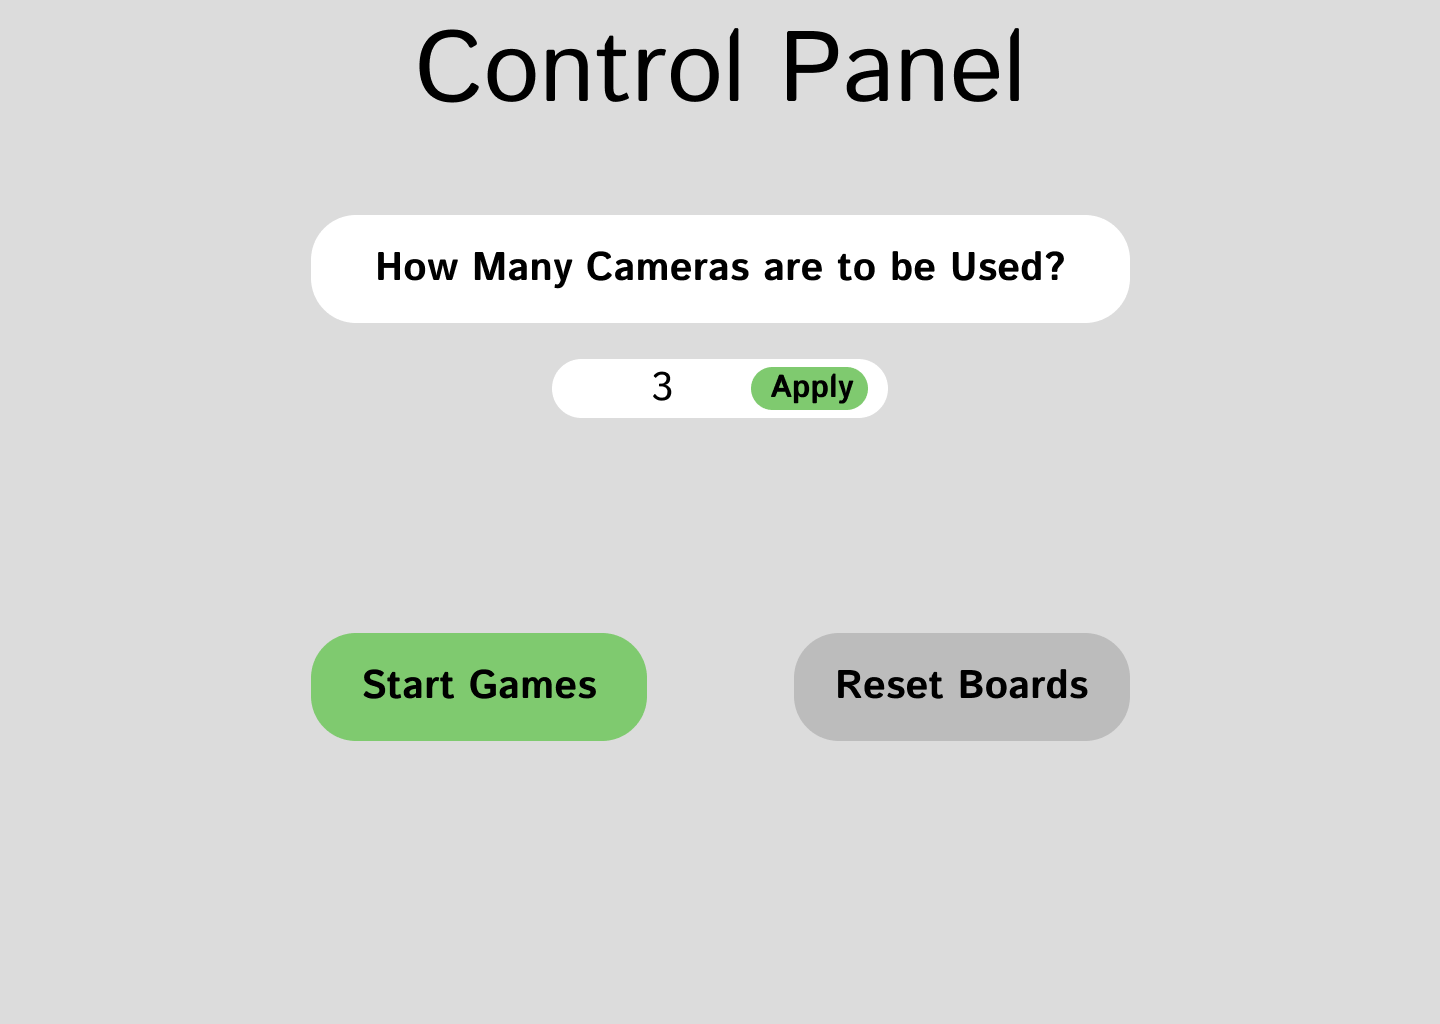
\includegraphics[width=\linewidth]{figures/methods/wireframes/control-panel-2.png}
        \caption{Step 2}
        \label{fig:control-panel-2}
    \end{subfigure}

    \begin{subfigure}[h!]{0.40\linewidth}
        \centering
        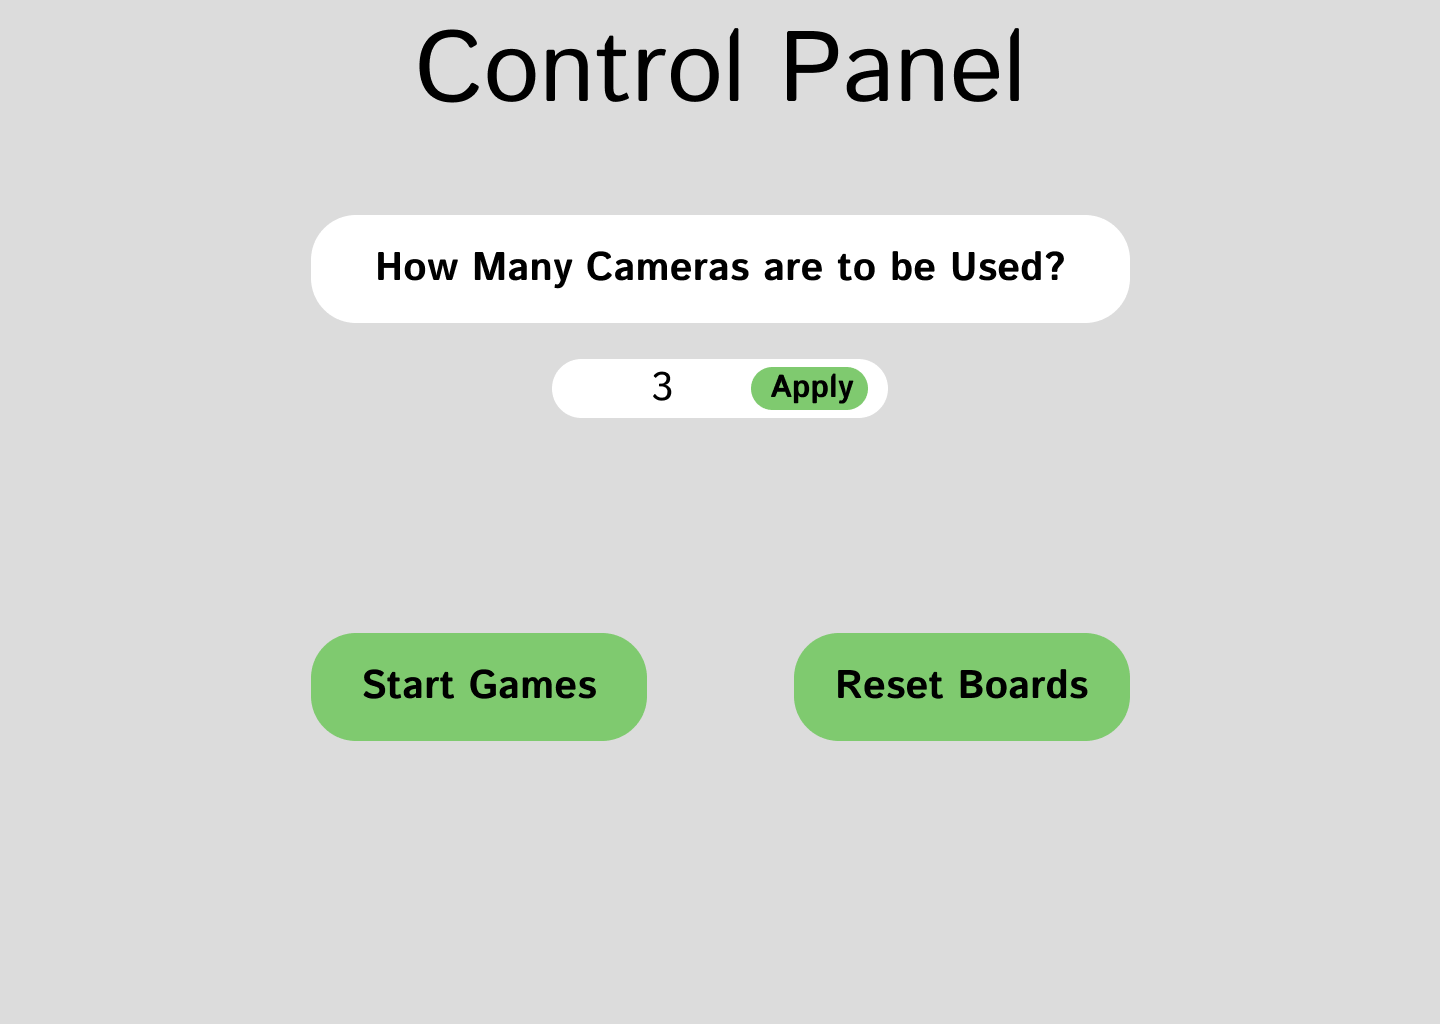
\includegraphics[width=\linewidth]{figures/methods/wireframes/control-panel-3.png}
        \caption{Step 3}
        \label{fig:control-panel-3}
    \end{subfigure}
    
    \caption[Control panel wireframes]{Control Panel wireframes showing sequential interaction steps.}
    \label{fig:control-panel-group}
\end{figure}


The client-side view is implemented as a web-based interface, developed in accordance with the accessibility principles described in Section \ref{sec:design}. The design prioritizes usability, aiming to offer a user-friendly and accessible experience for users across both desktop and mobile platforms. The interface is organized into two primary components: the tournament view and the board View. \\

The \textbf{tournament view} (see Figure \ref{fig:desktop-tournament-view}) provides a concise overview of all active games in the tournament. Its clean and minimal layout presents key information such as board numbers, player names, and a navigation button for accessing the corresponding board view. This approach ensures that users can quickly scan through the tournament and access gameswith minimal effort. \\

The \textbf{board view} (see Figure \ref{fig:desktop-board-view}) is focused on a single game, displaying both the live chessboard and a video stream of the ongoing game. The layout is designed for clarity, minimizing distractions so that users can easily follow the game in progress. \\

To ensure compatibility with mobile devices, the interface incorporates responsive design principles. On smaller screens, the tournament view simplifies its presentation by removing player names and retaining only the board number and navigation button (see Figure \ref{fig:phone-tournament-view}). This streamlined layout maintains usability without overwhelming the limited screen space.
Similarly, the board view adjusts to a vertical layout on mobile devices, stacking the chessboard and video stream one above the other (see Figure \ref{fig:phone-board-view}). This configuration enhances readability and preserves the overall clarity of the interface, even on compact displays.


\begin{figure}[h!]
\subsubsection*{Desktop View}
    \centering
    \begin{subfigure}[h!]{0.40\linewidth}
        \centering
        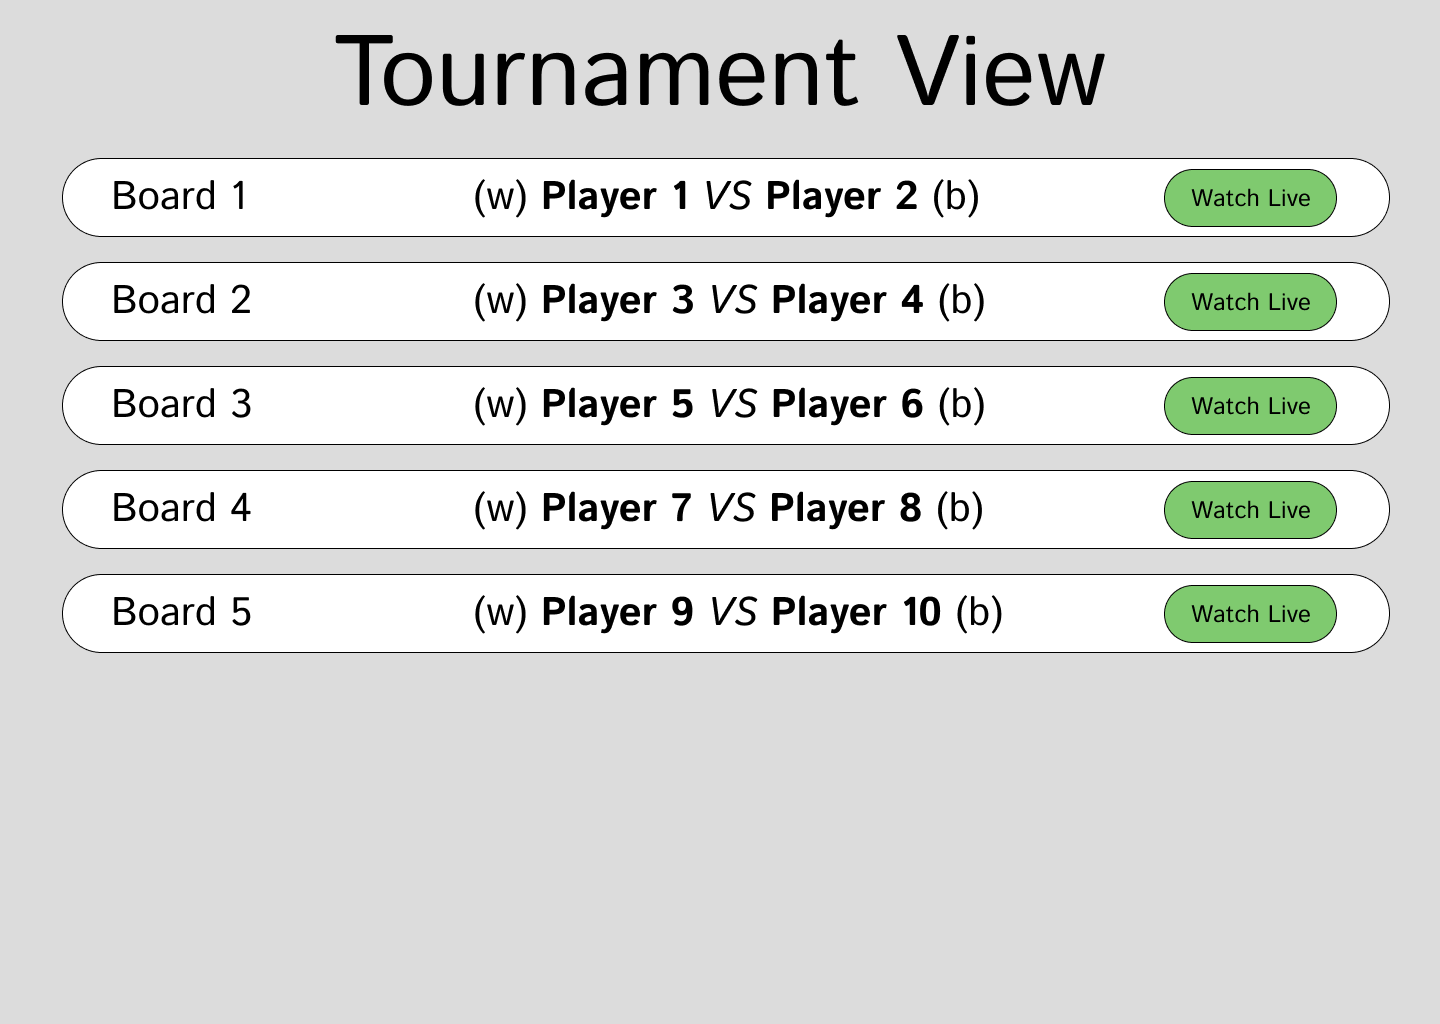
\includegraphics[width=\linewidth]{figures/methods/wireframes/desktop-tournament-view.png}
        \caption{Tournament view}
        \label{fig:desktop-tournament-view}
    \end{subfigure}
    \hfill
    \begin{subfigure}[h!]{0.40\linewidth}
        \centering
        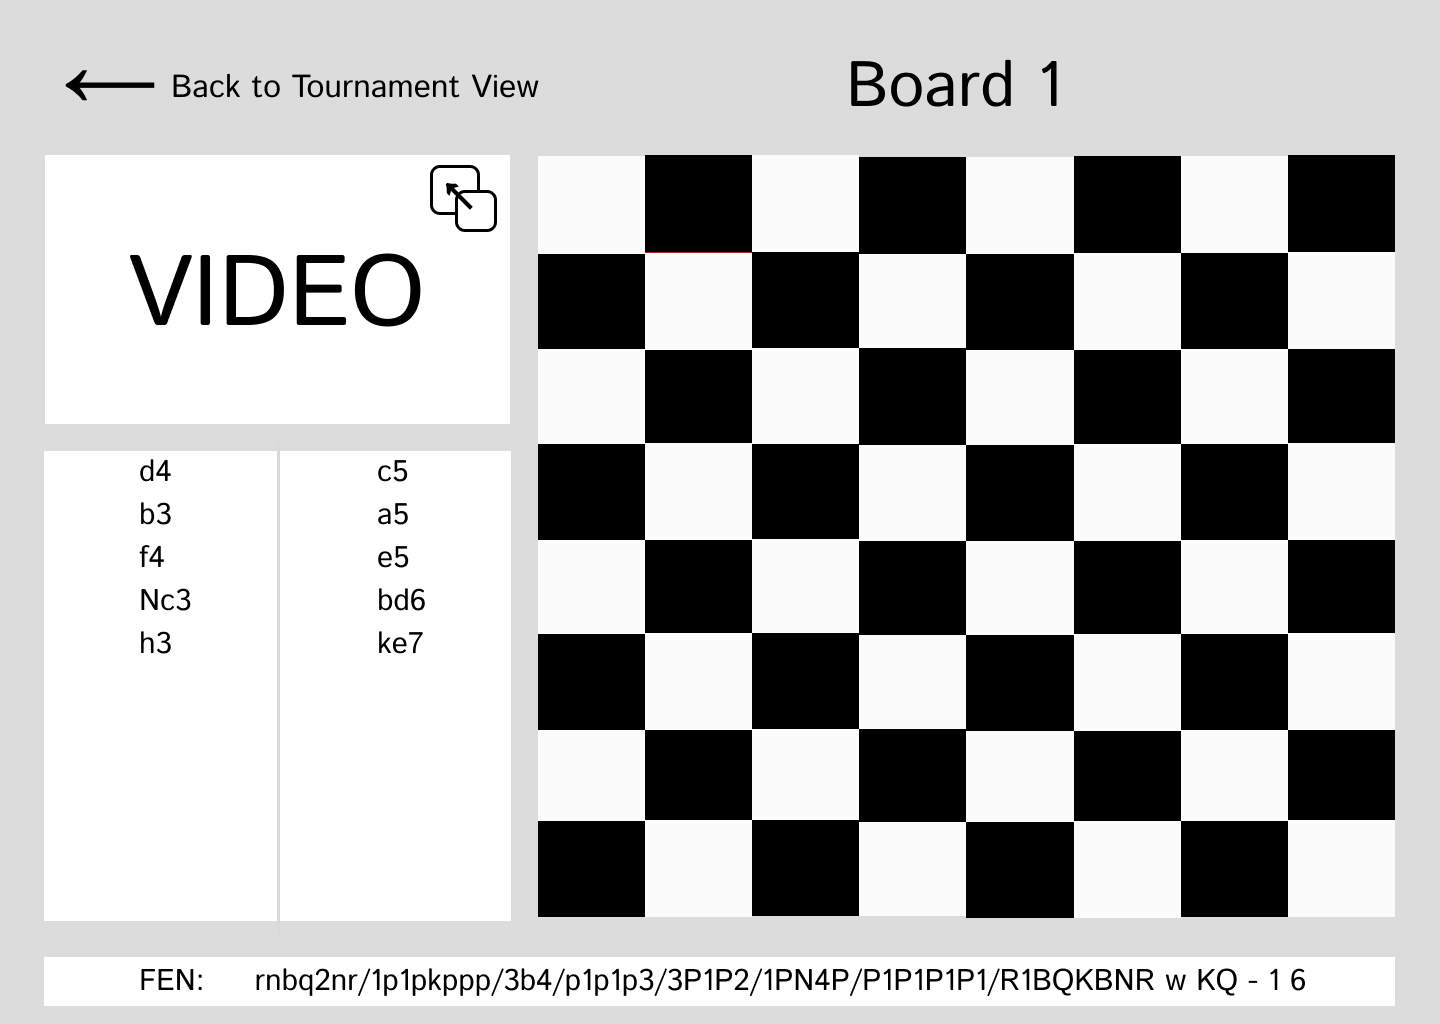
\includegraphics[width=\linewidth]{figures/methods/wireframes/desktop-board-view.png}
        \caption{Board view}
        \label{fig:desktop-board-view}
    \end{subfigure}

    \begin{subfigure}[h!]{0.40\linewidth}
        \centering
        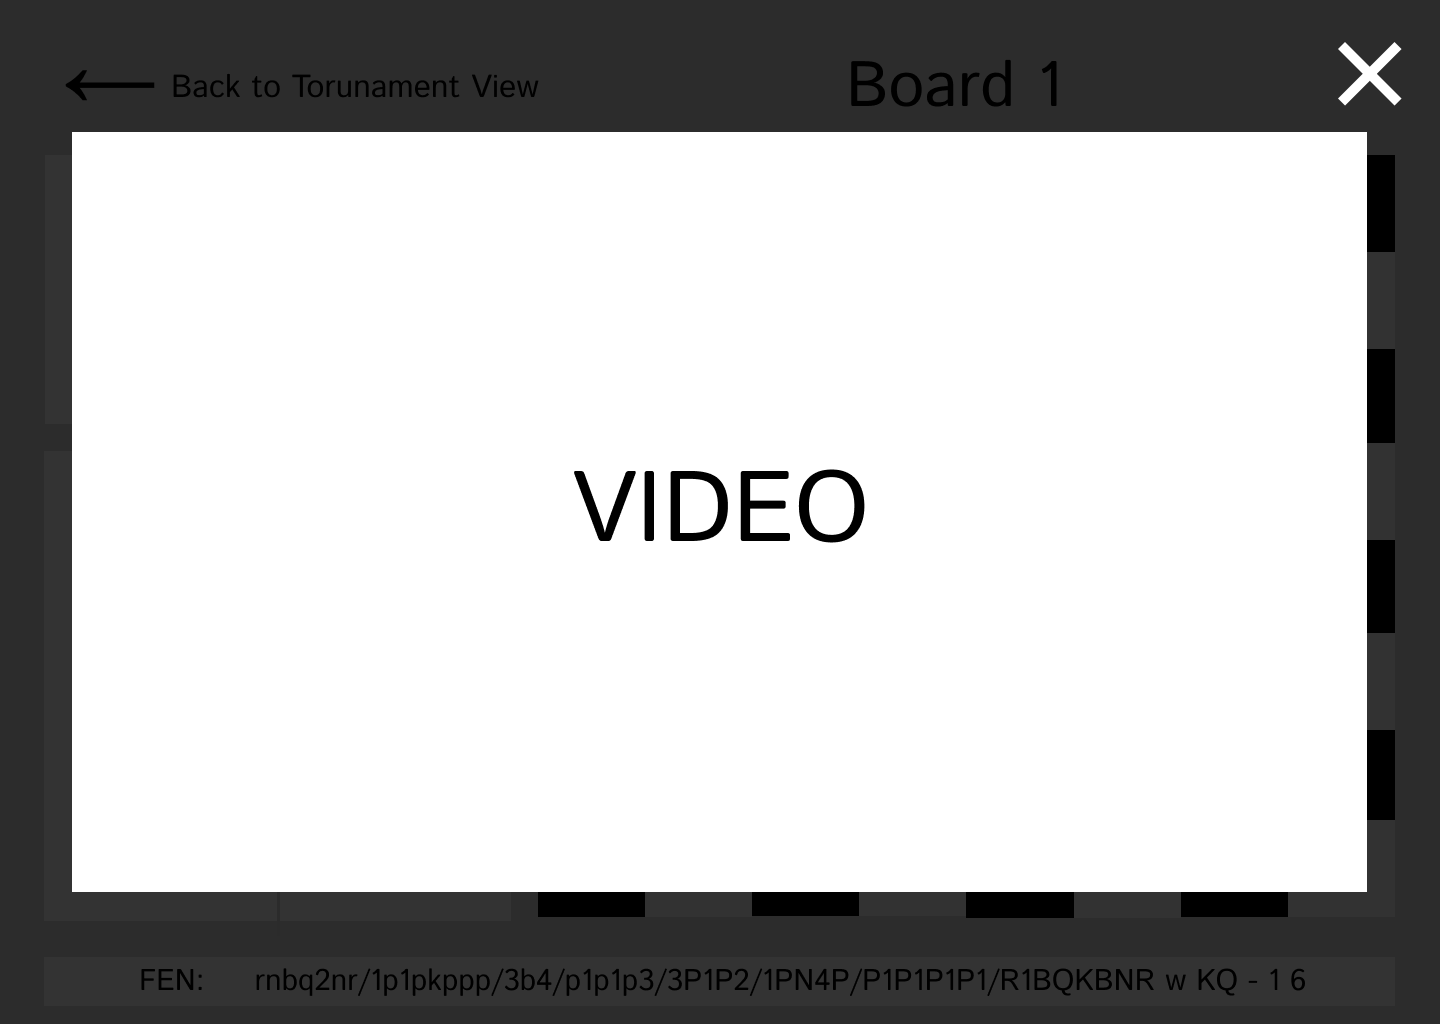
\includegraphics[width=\linewidth]{figures/methods/wireframes/desktop-full-screen-video-view.png}
        \caption{Fullscreen Video Feed}
        \label{fig:desktop-fullscreen-video}
    \end{subfigure}
    
    \caption[Desktop client-side wireframes]{Desktop client-side wireframes.}
    \label{fig:desktop-view-group}
\end{figure}


\begin{figure}[h!]
\subsubsection*{Phone View}
    \centering
    \begin{subfigure}[h!]{0.2\linewidth}
        \centering
        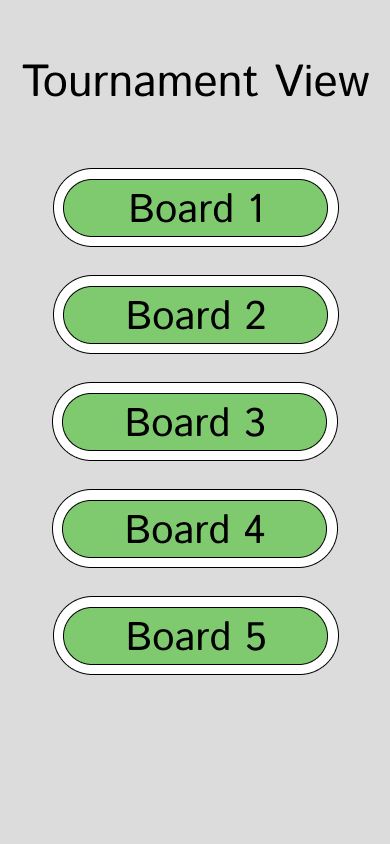
\includegraphics[width=\linewidth]{figures/methods/wireframes/phone-tournament-view.png}
        \caption{Tournament View}
        \label{fig:phone-tournament-view}
    \end{subfigure}
    \hfill
    \begin{subfigure}[h!]{0.2\linewidth}
        \centering
        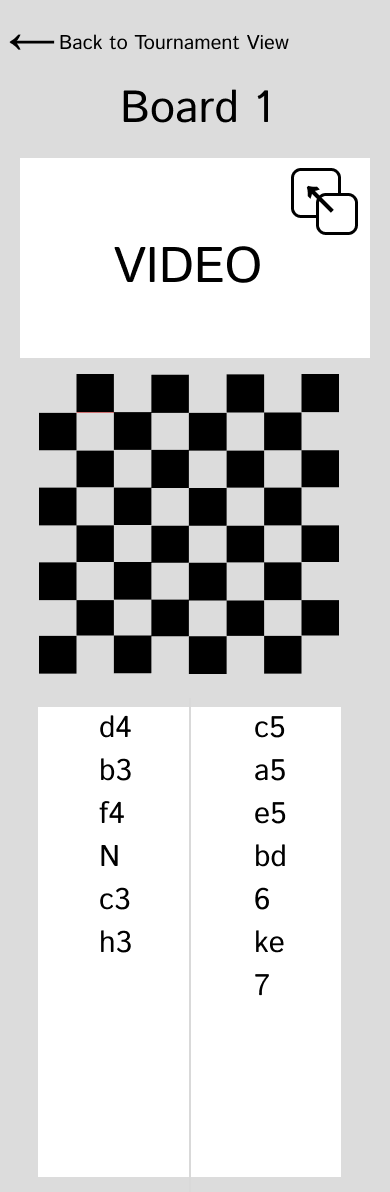
\includegraphics[width=\linewidth]{figures/methods/wireframes/phone-board-view.png}
        \caption{Board view}
        \label{fig:phone-board-view}
    \end{subfigure}
    \hfill
    \begin{subfigure}[h!]{0.2\linewidth}
        \centering
        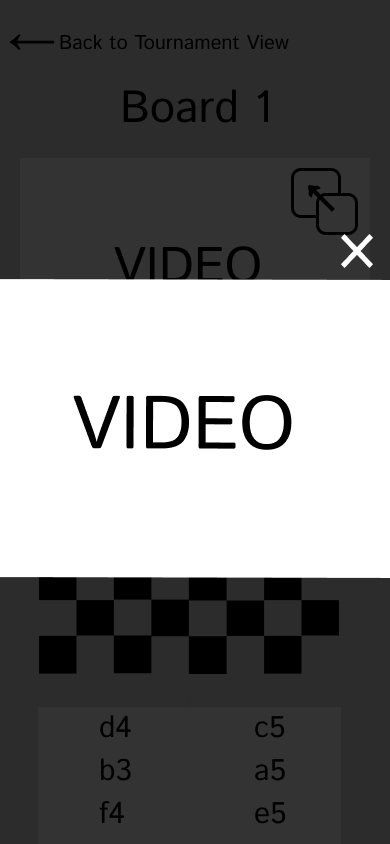
\includegraphics[width=\linewidth]{figures/methods/wireframes/phone-full-screen-video-view-vertical.png}
        \caption{Vertical Fullscreen Video Feed}
        \label{fig:phone-fullscreen-video-vertical}
    \end{subfigure}
    \hfill
    \begin{subfigure}[h!]{0.2\linewidth}
        \centering
        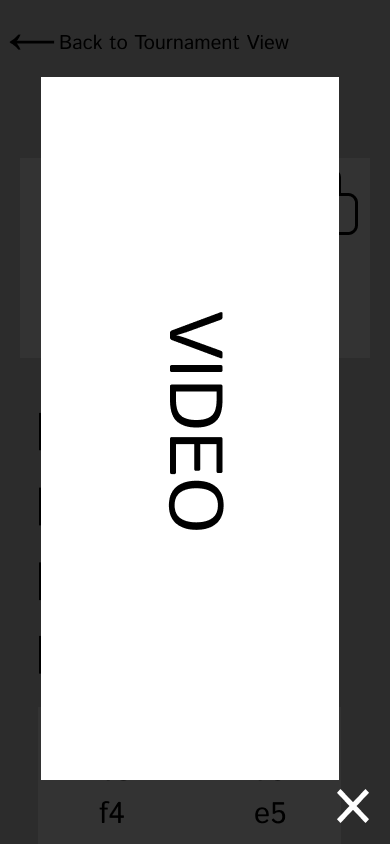
\includegraphics[width=\linewidth]{figures/methods/wireframes/phone-full-screen-video-view-horizontal.png}
        \caption{Horizontal Fullscreen Video Feed}
        \label{fig:phone-fullscreen-video-horizontal}
    \end{subfigure}
    
    \caption[Phone client-side wireframes]{Phone client-side wireframes.}
    \label{fig:phone-view-group}
\end{figure}

\newpage

\section{Project Management}
\label{sec:methods-project-management}
The team adopted the \gls{scrum} framework to organize the project and coordinate tasks effectively. Work was divided into biweekly sprints, each beginning with a planning session where prioritized items were selected from the product backlog. Tasks were then broken down into manageable units and assigned to individual team members. The sprint goals guided the development process, culminating in a sprint review and retrospective at the end of each cycle to assess outcomes and reflect on team performance. \\

To support this workflow, a meeting routine was established. Internal team meetings were held as needed to discuss progress, resolve blockers, and coordinate efforts. Additionally, brief informal stand-up meetings took place during office hours to maintain shared awareness of current tasks and priorities. Biweekly meetings with the supervisor ensured ongoing guidance and alignment with academic requirements. Meetings with the product owner occurred approximately once or twice per month, providing opportunities to present progress and gather valuable feedback. \\

To support effective collaboration, responsibilities were divided among team members. Roles included communication lead, meeting minute writer, and documentation manager. The distribution of roles helped maintain a consistent workflow and ensured accountability across different project areas. All meeting minutes were documented and stored in the project repository alongside the main report. Sprint reviews, retrospectives, and other supplementary documentation, including the project timetable, testing data, and contact log, were maintained in a shared OneDrive folder. \\

Communication was primarily facilitated through Discord, which served as the team's communication platform. This included informal discussions and quick coordination on tasks and meeting times within the team. Email was used for formal communication and documentation, such as scheduling meetings with the supervisor or product owner. \\

GitHub was used for both version control and task management. Issues in GitHub were used to define and track units of work. These were categorized and organized using labels. Each issue could be assigned, prioritized, and monitored through a visual interface. GitHub pull requests also enabled peer review of code contributions before integration. All code contributions and associated tasks were managed through GitHub's branching model. This allowed team members to work independently on features and bugs, while maintaining a clean and stable main branch. \\

\section{Tools and Platforms}
\label{sec:tools-and-platforms}

\subsection*{Development Tools}
\label{subsec:development-tools}

\begin{itemize}
    \item \textbf{\acrlong{vscode}} was used as the primary development environment due to its support for multiple programming languages and extensions.
\item \textbf{Postman} was employed for testing and validating \acrshort{rest}ful \glspl{api}, utilizing built-in JavaScript-based test snippets.
\item \textbf{Netron.app} was used to visualize neural network architectures during the evaluation phase.
\item \textbf{Git} facilitated version control and collaboration throughout the development process.
\item \textbf{\glspl{llm}} (for example ChatGPT) were consulted to review code and provide suggestions, functioning as a collaborative assistant.
\item \textbf{Lighthouse} was used to evaluate and improve the performance and accessibility of the developed web interface.
\end{itemize}.

\subsection*{Collaboration Tools}
\label{subsec:collaboration-and-design-tools}

\begin{itemize}
    \item \textbf{GitHub} was used for its integrated project management features, enabling the team to create an Issue Board for efficient tracking of tasks. It was also used for code reviews and version control.

    \item \textbf{Figma} was used as a tool for sketching and creating wireframes.
    
    \item \textbf{OneDrive} was used as a platform for storing and sharing files.
    
    \item \textbf{Overleaf} was used as the platform for writing the report, utilizing its LaTeX support to efficiently compose and format the thesis.
\end{itemize}

\newpage

\section{Technology Stack}
\label{sec:technology-stack}

\subsection*{Backend}

Python was selected for the project’s backend because of its simple and user-friendly syntax. Its extensive ecosystem of libraries and frameworks reduces development time. Furthermore, Python’s community and industry provide valuable resources for \gls{api} development and \gls{ml} capabilities.

\subsubsection*{Python Libraries}

\begin{itemize}
    \item \textbf{chess} - Used for move generation, validation, and parsing of chess game formats \cite{python:chess}.
    \item \textbf{FastAPI} - Web framework used to develop \acrshort{rest}ful \glspl{api} for backend services \cite{python:fastapi}.
    \item \textbf{numpy} - Package for numerical operations \cite{python:numpy}.
    \item \textbf{onnxruntime} - Used for running pre-trained \gls{ml} models \cite{python:onnx}.
    \item \textbf{opencv-python} - Utilized for computer vision tasks \cite{python:opencv}.
    \item \textbf{requests} - Used to handle \gls{http} communication \cite{python:requests}.
    \item \textbf{scipy} – Employed for scientific and numerical computations \cite{python:scipy}.
    \item \textbf{tensorflow} - Used to build and execute \gls{ml} models \cite{python:tensorflow}.
    \item \textbf{customtkinter} - Desktop \gls{ui} built with a modern Tkinter-based library offering customizable widgets. \cite{python:ctk}
\end{itemize}


\subsection*{Frontend}

TypeScript was selected for the project's frontend language due to it's type-safety, as discussed in Section \ref{subsec:type-safety}.

\subsubsection*{TypeScript Dependencies}

\begin{itemize}
    \item \textbf{Vite} - A fast frontend build tool for web applications \cite{ts:vite}.
    
    \item \textbf{React} - Builds user interfaces from individual pieces called components \cite{ts:react}.
    
    \item \textbf{\acrshort{swc}} - Speeds up the Vite development server \cite{ts:swc}.
    
    \item \textbf{chess.ts} - A TypeScript chess library for handling game logic including move validation and piece management \cite{ts:chess}.
    
    \item \textbf{react-dom} - Serves as the entry point to the DOM and server renderers for React \cite{ts:react-dom}.
\end{itemize}

\newpage

\section{Testing}
\label{sec:testing}

\subsection{Model Testing}
\label{subsec:model-testing}
The performance of the \gls{ml} model was evaluated through 100 test  games. Five distinct chess openings were selected, with 10 games played per opening on each of two board types: plastic and wooden. This resulted in 50 games per board type. Each game consisted of 15 full moves, corresponding to 15 moves by white and 15 moves by black. \\

Each move was logged as either successful or unsuccessful. A 30-second window was provided for the model to detect and transmit each move, starting from the moment the move was made \gls{otb}. If the model failed to detect the move within this time frame, or if it detected the wrong move, it was marked as unsuccessful. The game concluded either when a move was marked unsuccessful or all 15 full moves had been completed. \\

The webcam was mounted above the board at an angle of approximately 60–70\si{\degree} relative to the table surface. The white pieces were placed on the left side of the camera's field of view, and the black pieces on the right.

\begin{figure}[h!]
    \centering
    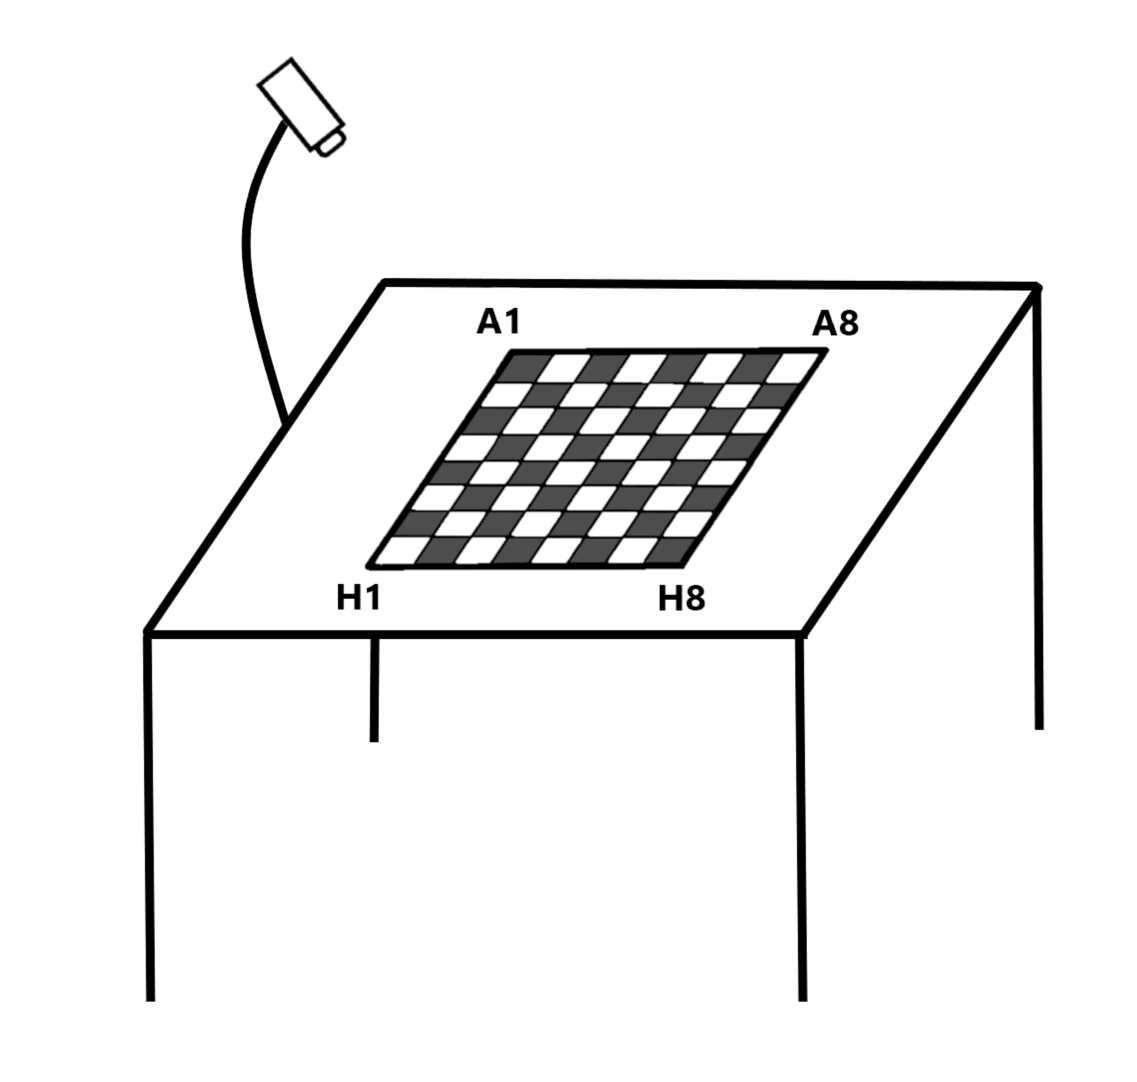
\includegraphics[width=0.65\linewidth]{figures/methods/testing/setup.png}
    \caption[Setup during testing]{Physical setup during testing, showing the board, camera position, and piece orientation.}
    \label{fig:setup}
\end{figure}

\newpage

\subsection{API}
\label{subsec:api-methods}

\subsubsection*{WebSocket Testing (Live Data Simulation)}
\label{subsubsec:websocket-methods}

To test real-time communication via WebSocket, a lightweight simulator was implemented. The simulator sequentially sent hard-coded chess moves to connected clients, emulating live gameplay data. The frontend application was connected to the WebSocket endpoint during testing, enabling it to receive and display incoming data. This setup allowed for effective verification of the WebSocket functionality and ensured that the frontend was capable of handling and rendering live move updates as intended.

\subsubsection*{REST API Testing with Postman}
\label{subsubsec:rest-api-methods}

To verify the correctness of the \gls{rest}ful \gls{api} endpoints, Postman was used as a manual testing tool. Postman enables direct interaction with \gls{http} endpoints, making it well-suited for verifying both request structures and server responses. Each implemented endpoint was tested individually, including operations such as resetting specific boards, resetting all boards simultaneously, retrieving the list of active boards, and streaming video from individual board cameras. \\

Figure~\ref{fig:postman-rest-tests} illustrates sample \gls{api} calls tested through Postman. Various \texttt{POST} and \texttt{GET} requests were issued to endpoints such as \texttt{/reset/1}, \texttt{/video/1}, and \texttt{/boards}. These tests confirmed that backend services responded as expected, returning successful status codes, valid response payloads, and triggering the intended state changes. This form of manual \gls{rest} testing ensured \gls{api} correctness prior to frontend integration.

\begin{figure}[h!]
    \centering
    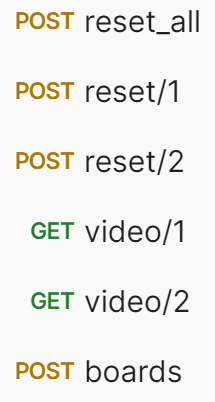
\includegraphics[width=0.25\linewidth]{figures//methods/postman-light.png}
    \caption[Postman REST API tests]{Postman \gls{rest} \gls{api} tests.}
    \label{fig:postman-rest-tests}
\end{figure}

\subsection{Wireframe Testing}
\label{subsubsec:user-centered-design}

The usability testing process followed principles discussed in Section \ref{subsec:testing}. At the early stage of the design process, wireframe testing was conducted with a small but diverse group of users. The aim was to evaluate whether the interface was intuitive, and whether the sizing and layout were appropriate for a range of users. \\

Participants included individuals from various age groups (ranging from 18 to 55) and backgrounds, including both experienced chess players and those unfamiliar with the game. Their technical experience also varied, from computer science students to non-technical individuals such as stay-at-home parents. In total, eight participants were involved in this test, excluding the developers and stakeholders of the project. \\

Before testing began, all participants were presented with the following scenario to establish context:

\begin{quote}
\textit{You are viewing a chess game between two companions you know. You visit the tournament organizer's website and come across this webpage.}
\end{quote}

Participants were then asked to either complete a set of predefined tasks or freely explore the interface, simulating a real-world browsing scenario. This approach was designed to assess how naturally users could navigate the interface without guidance. \\

After their interaction with the wireframe, participants completed an anonymous feedback form, which included the following questions:

\begin{itemize}
    \item \textit{On a scale from 1 to 5, how satisfied are you with the overall experience of the application?}
    \item \textit{On a scale from 1 to 5, how satisfied are you with the tournament View page?}
    \item \textit{On a scale from 1 to 5, how satisfied are you with the board view page?}
    \item \textit{Do you have any feedback, suggestions for improvement, or features you would like to see added?}
\end{itemize}

See Section \ref{subsec:wireframe} for the tested wireframe.



\subsection{Color Palette Testing}
\label{subsubsec:color-palette}

In selecting the application’s color palette, the group opted for a variation of blue. This choice was influenced by the symbolic associations of the color blue, which is linked to imagination, intelligence, and wisdom \cite{blue}. These are traits that are relevant to the game of chess \cite{chess:ppqty, chess:chess-and-creativity}. \\

To identify the most suitable stylistic direction, several versions of the application were developed, each featuring a distinct color palette. These prototypes were printed and displayed in a shared space, allowing individuals from diverse backgrounds to view and compare them. Participants were invited to vote for their preferred versions through a form. Each participant was allowed up to three votes and had the option to leave comments.
\cleardoublepage

\chapter{Results}

\begin{center}
    \textit{This chapter presents the outcomes of the project, including the functionality and performance of the developed application. It highlights the achieved results in relation to the project goals and requirements.}
\end{center}

\section{Overview of Delivered Product}
The application was developed as an open-source project with the intention that the code can be reused, maintained, and extended by others. All components are built using open and freely available technologies, ensuring that the system can be installed on local hardware without the need for licensed software or cloud-based services. This aligns with the requirement that all processing should be performed locally, using common hardware such as a webcam connected to a local machine running either Windows or Ubuntu. \\

The project follows clear coding standards and development best practices, making the code easy to understand and modify. All functionality is well documented, enabling future developers to build upon the existing solution. For example, to support new chess variants, integrate additional hardware, or improve the recognition models. To support future development and accessibility, the source code is published in a public Git repository without restrictions on reuse or adaptation. \\

The application itself is a local, camera-based system for digitalizing over-the-board chess games in real-time. It detects piece movements on a physical chessboard using image recognition and converts the game into a \gls{pgn} file, which can be viewed or analyzed digitally. The system operates entirely on local hardware, with a front-end interface that allows users to follow games live and a back-end that manages board recognition and game logic. The application is designed to be low-cost, open-source, and easy to maintain, with extensibility in mind for future features. \\

The delivered product refers to the final version of the application submitted at the conclusion of this Bachelor’s thesis. The application was developed at the request of the product owner and based on the requirements provided. The initial description served as a general concept rather than a detailed specification, which meant that decisions regarding design, architecture, and technology were left to the development team. Throughout the development process, ideas and design choices were discussed with the product owner and approved during regular meetings.

\section{Detection Performance Models}
\label{chesscam-metrics}
As a baseline for evaluating detection performance, results from ChessCam repository were first considered \cite{github:chesscam}. These metrics represent the upper-bound performance of the models under ideal conditions. \\

Figure~\ref{fig:chesscam-piece-metrics} illustrates the performance of the piece detection model, which demonstrates consistently high precision and recall throughout training. Both metrics rapidly converge above 0.95, indicating stable and reliable detection \cite{wandb:piece-detection}. In contrast, Figure~\ref{fig:chesscam-xcorners-metrics} presents the results for xcorners detection, showing moderately lower performance. Precision and recall improve steadily over time and stabilize at approximately 0.8 and 0.75, respectively \cite{wandb:xcorner-detection}. \\

\begin{figure}[H]
\centering
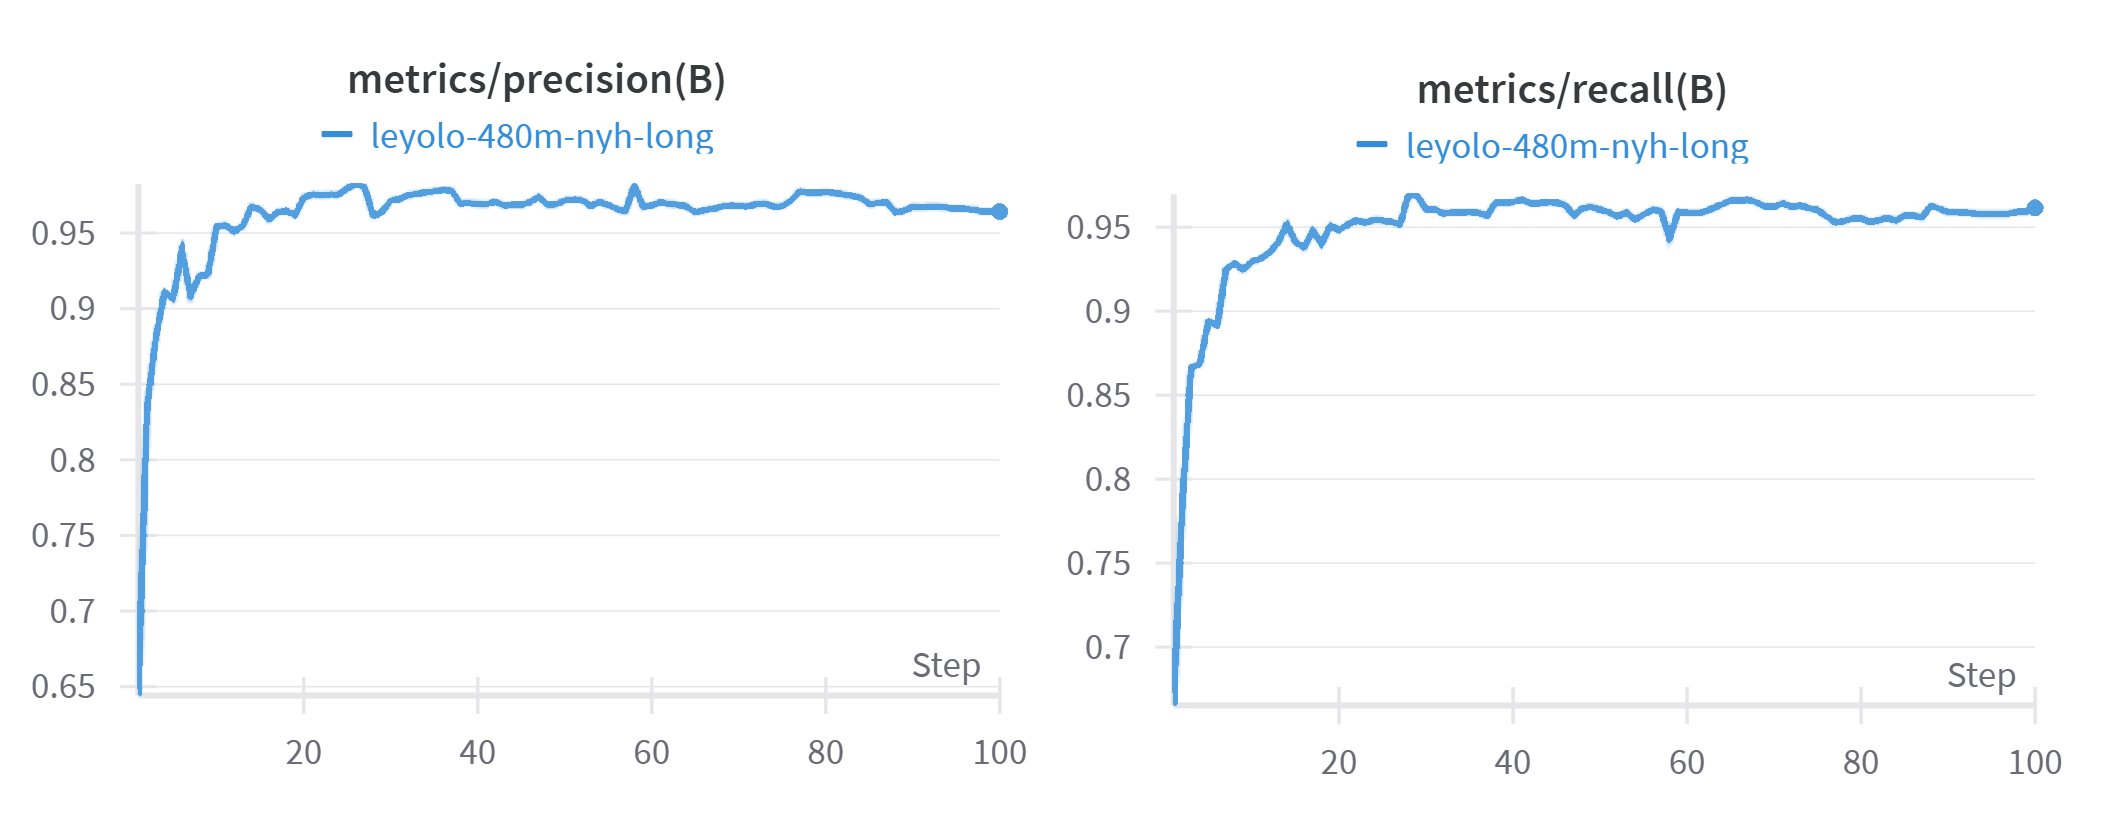
\includegraphics[width=\textwidth]{figures/results/machine-learning/piece-metrics.png}
\caption[Performance piece detection (ChessCam)]{Performance metrics for piece detection from ChessCam repository \cite{wandb:piece-detection}.}
\label{fig:chesscam-piece-metrics}
\end{figure}

\begin{figure}[H]
\centering
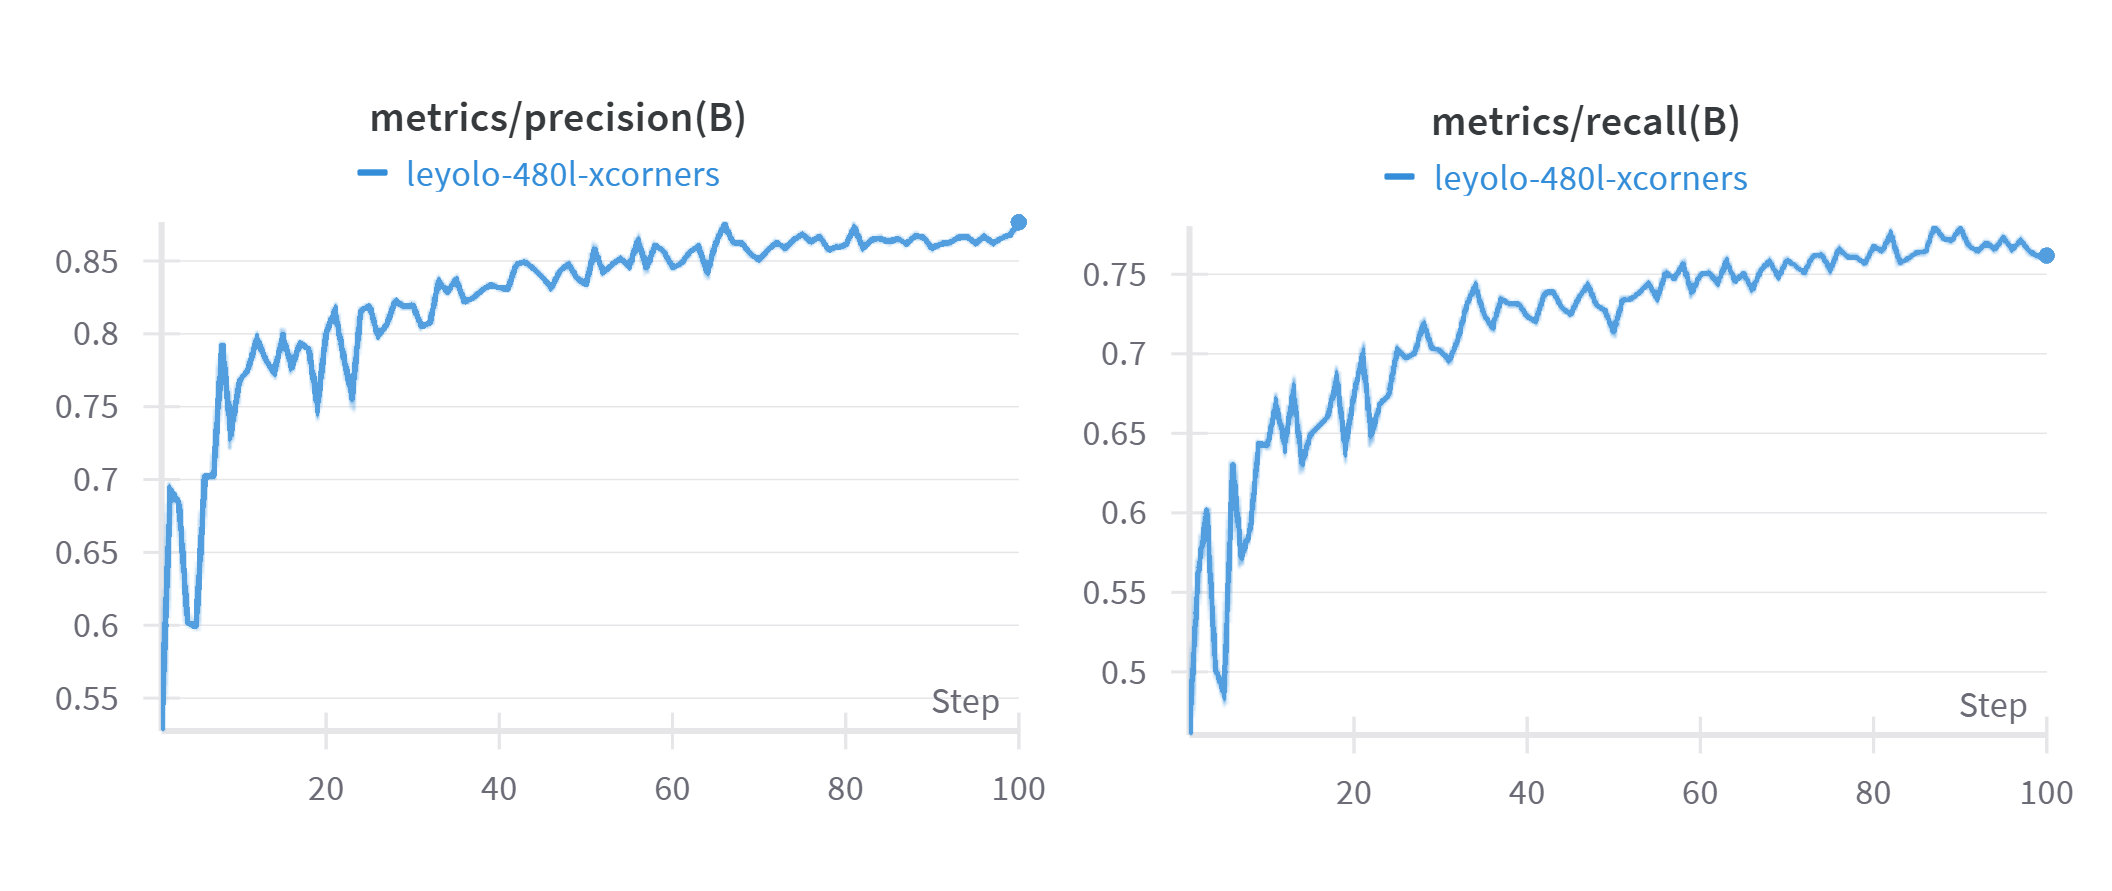
\includegraphics[width=\textwidth]{figures/results/machine-learning/xcorners-metrics.png}
\caption[Performance xcorners detection (ChessCam)]{Performance metrics for xcorners detection from ChessCam repository \cite{wandb:xcorner-detection}.}
\label{fig:chesscam-xcorners-metrics}
\end{figure}

\section{API}
% To support continuous communication between the backend and frontend, the application establishes a WebSocket connection. This communication channel is used for transmitting move data as it is detected by the board recognition system. Unlike traditional \gls{http} requests, which operate on a request-response basis, WebSocket allows for continuous, two-way communication between the server and the client as described in \ref{subsubsec:websocket} \\

% Once the application initiates a connection, the WebSocket remains open throughout the session. As new moves are identified on the physical board, the backend sends the corresponding move data as messages through the WebSocket. These messages are then received by the frontend, which updates the displayed move list and board state in real-time. \\

% The WebSocket server also processes specific command messages to manage game state. For instance, a message labeled \texttt{RESET} prompts the frontend to clear the current move list, signaling the start of a new game, while simultaneously resetting the backend to prepare for a new tournament round. Conversely, a message labeled \texttt{INVALID} indicates an unrecognized or illegal move and does not result in any frontend updates. 

\begin{table}[h!]
    \centering
    \caption[API endpoint overview]{Overview of available FastAPI REST and WebSocket endpoints for board control and video streaming}
    \label{tab:api-endpoints}
    \begin{tabular}{L{0.15\linewidth}L{0.25\linewidth}L{0.5\linewidth}}
        \toprule
        \textbf{Method} & \textbf{Endpoint} & \textbf{Description} \\
        \midrule
        \texttt{POST} & \texttt{/reset/\{board\_id\}} & Resets a specific chess board by ID. \\
        \texttt{POST} & \texttt{/reset\_all} & Resets all boards in memory. \\
        \texttt{GET} & \texttt{/boards} & Returns a list of all active board IDs. \\
        \texttt{GET} & \texttt{/video/\{id\}} & Streams \gls{mjpeg} video from a specific camera (board ID). \\
        \texttt{WebSocket} & \texttt{/moves/\{board\_id\}} & Sends live chess move updates to subscribed WebSocket clients. \\
        \bottomrule
    \end{tabular}
\end{table}

% \begin{code}[h!]
% \caption{Reset Specific Board}
% \label{code:reset-specific-board}
% \lstinputlisting[language=Python, firstline=9, lastline=17]{code/backend/logic/api/routes/admin_routes.py}
% \end{code}

% \begin{code}[h!]
% \caption{Reset All Boards}
% \label{code:reset-specific-board}
% \lstinputlisting[language=Python, firstline=19, lastline=23]{code/backend/logic/api/routes/admin_routes.py}
% \end{code}

% \begin{code}[h!]
% \caption{Get List of All Active Boards}
% \label{code:get-boards-list}
% \lstinputlisting[language=Python, firstline=25, lastline=29]{code/backend/logic/api/routes/admin_routes.py}
% \end{code}

% \begin{code}[h!]
% \caption{Get Video Feed}
% \label{code:video-feed}
% \lstinputlisting[language=Python, firstline=7, lastline=20]{code/backend/logic/api/routes/video_routes.py}
% \end{code}

% \begin{code}[h!]
% \caption{WebSocket route}
% \label{code:websocket}
% \lstinputlisting[language=Python, firstline=6, lastline=27]{code/backend/logic/api/routes/websocket_routes.py}
% \end{code}



\section{Frontend}
\label{subsec:results-frontend}
The frontend of the application serves as the user interface. It includes a control panel for tournament organizers and a web application for spectators. The application's responsibility is to visualize the chessboard and display ongoing moves. The frontend communicates with the backend via WebSocket to ensure real-time updates. \\

The control panel is a standalone administrative interface used by tournament organizers to configure and manage the tournament setup. It allows the organizer to select the number of cameras, initiate the tournament, and reset boards between rounds, as shown in Figure~\ref{fig:control-panel}. This interface ensures the centralized management of tournament operations. \\

\begin{figure}[h!] \centering 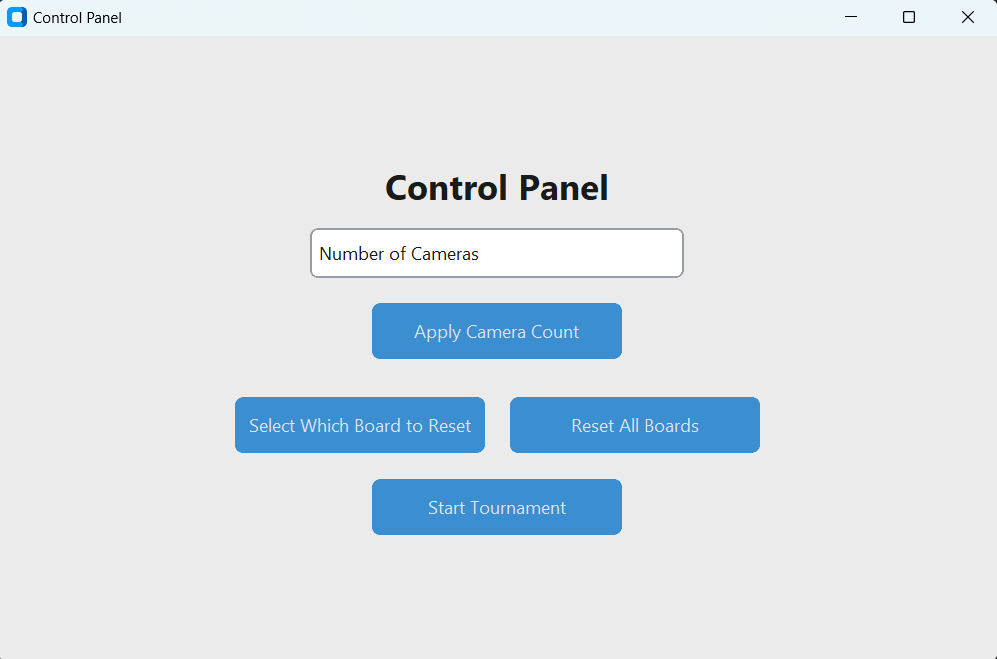
\includegraphics[width=0.75\linewidth]{figures/results/frontend/control-panel/control-panel.png} \caption[Display of control panel]{The control panel used by the tournament organizers.}\label{fig:control-panel} \end{figure}

Once the application is launched, the accompanying web application becomes accessible to spectators. It is designed to allow viewers to follow the tournament across a range of devices. Spectators can navigate between views, observe live games, and explore additional information about the system. Built as a responsive interface, it adapts to both desktop and mobile screens to ensure accessibility and usability. \\

The landing page is the tournament view. The tournament view presents an overview of all ongoing games. Each entry shows the board number, the players' names and ratings, and a link to follow the game live, as shown in Figure~\ref{fig:tournament-view-mocked}. \\

\begin{figure}[h!] \centering \fbox{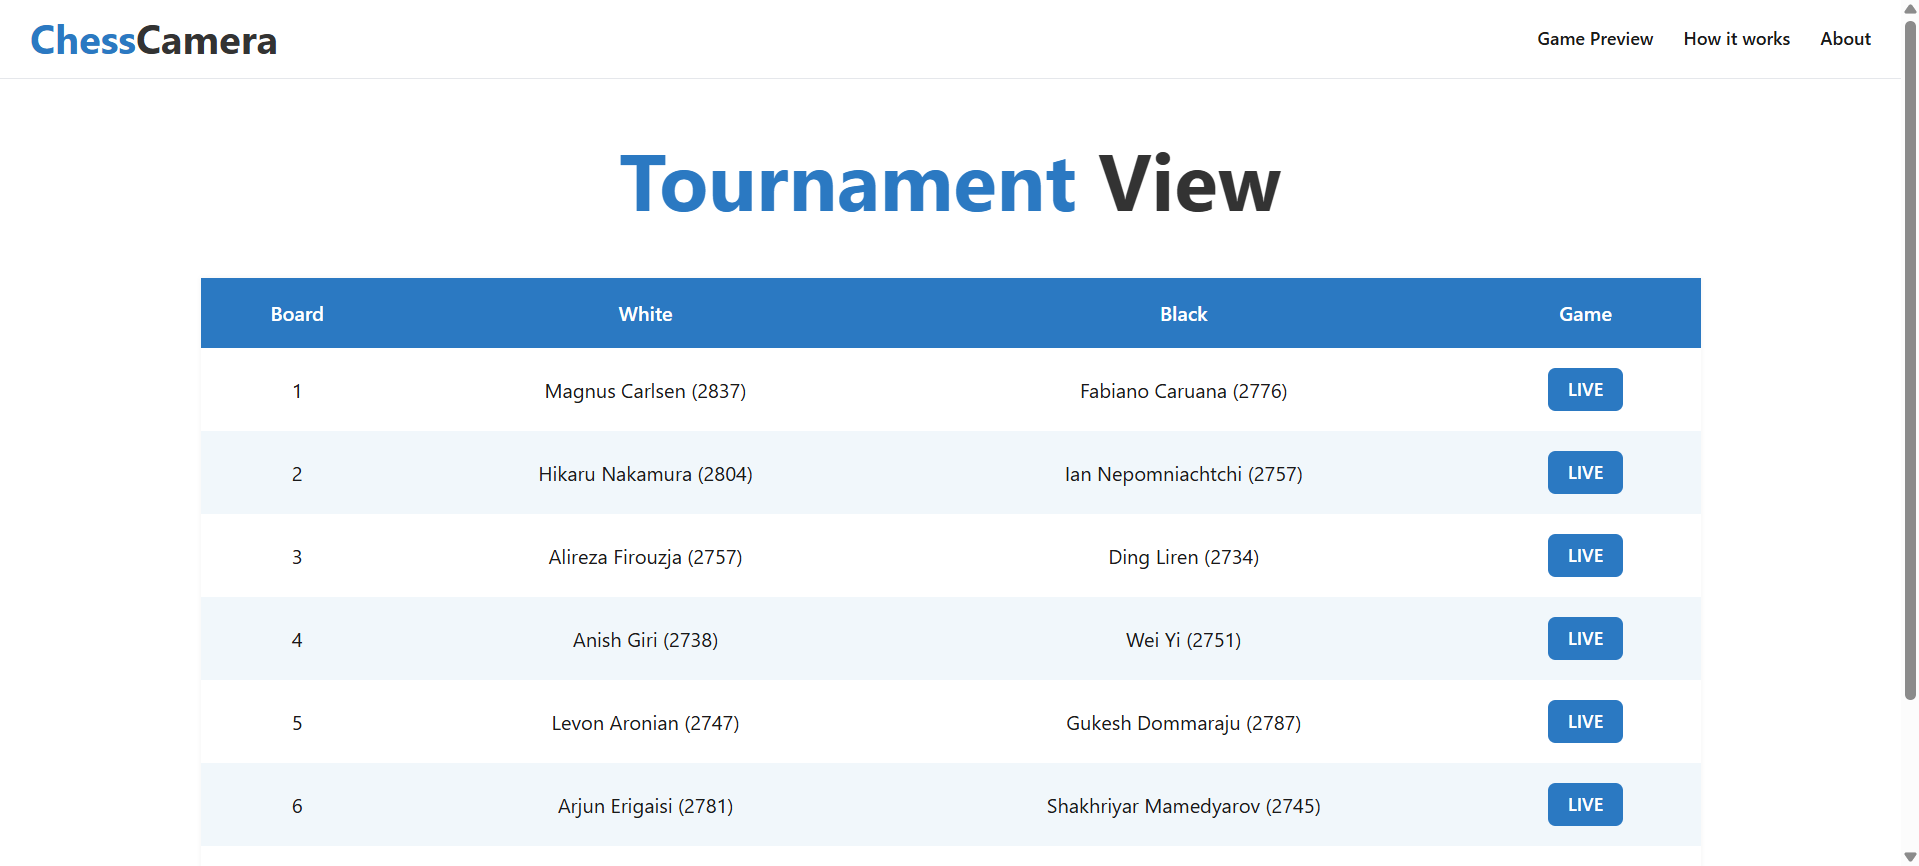
\includegraphics[width=0.75\linewidth]{figures/results/frontend/tournament-view/mocked.png}}\caption[Display of tournament view]{A mocked demonstration of tournament view.}\label{fig:tournament-view-mocked} \end{figure}

Another page is the game preview, which displays miniature boards for multiple games. This view provides an overview of all active games, allowing users to quickly identify and select any game for detailed viewing, as shown in Figure~\ref{fig:game-preview}. It offers an efficient way to stay updated on several games at once. \\

\begin{figure}[h!] \centering \fbox{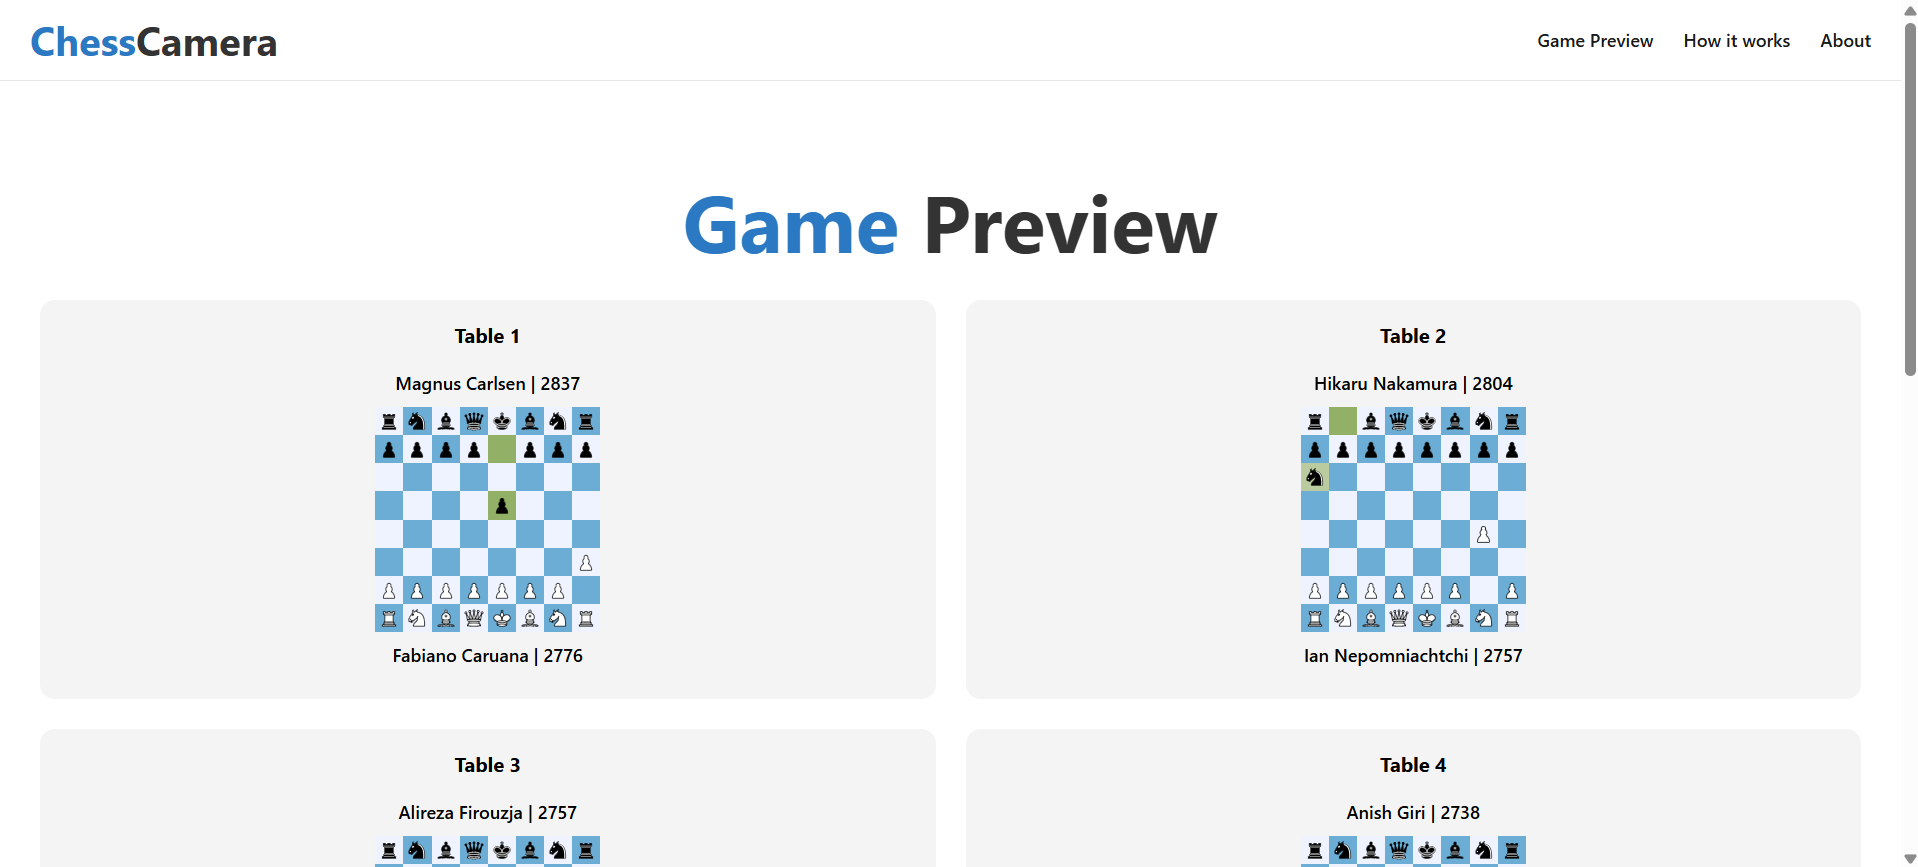
\includegraphics[width=0.75\linewidth]{figures/results/frontend/game-preview/desktop.png}}\caption[Display of game preview]{A mocked demonstration of game preview.}\label{fig:game-preview} \end{figure}

One of the main pages in the web application is the the board view. The board view presents a detailed view of a single game. It features a digital chessboard, a list of moves played, a live camera feed, and an evaluation bar, as shown in Figure~\ref{fig:download-pgn}. The elements update in real-time, creating an engaging experience for users. On the Board View page, users can download the \gls{pgn} file of the current game via a dedicated button, which saves the file locally. The board view is shown in Figure~\ref{fig:download-pgn}. \\

\begin{figure}[h!] \centering \fbox{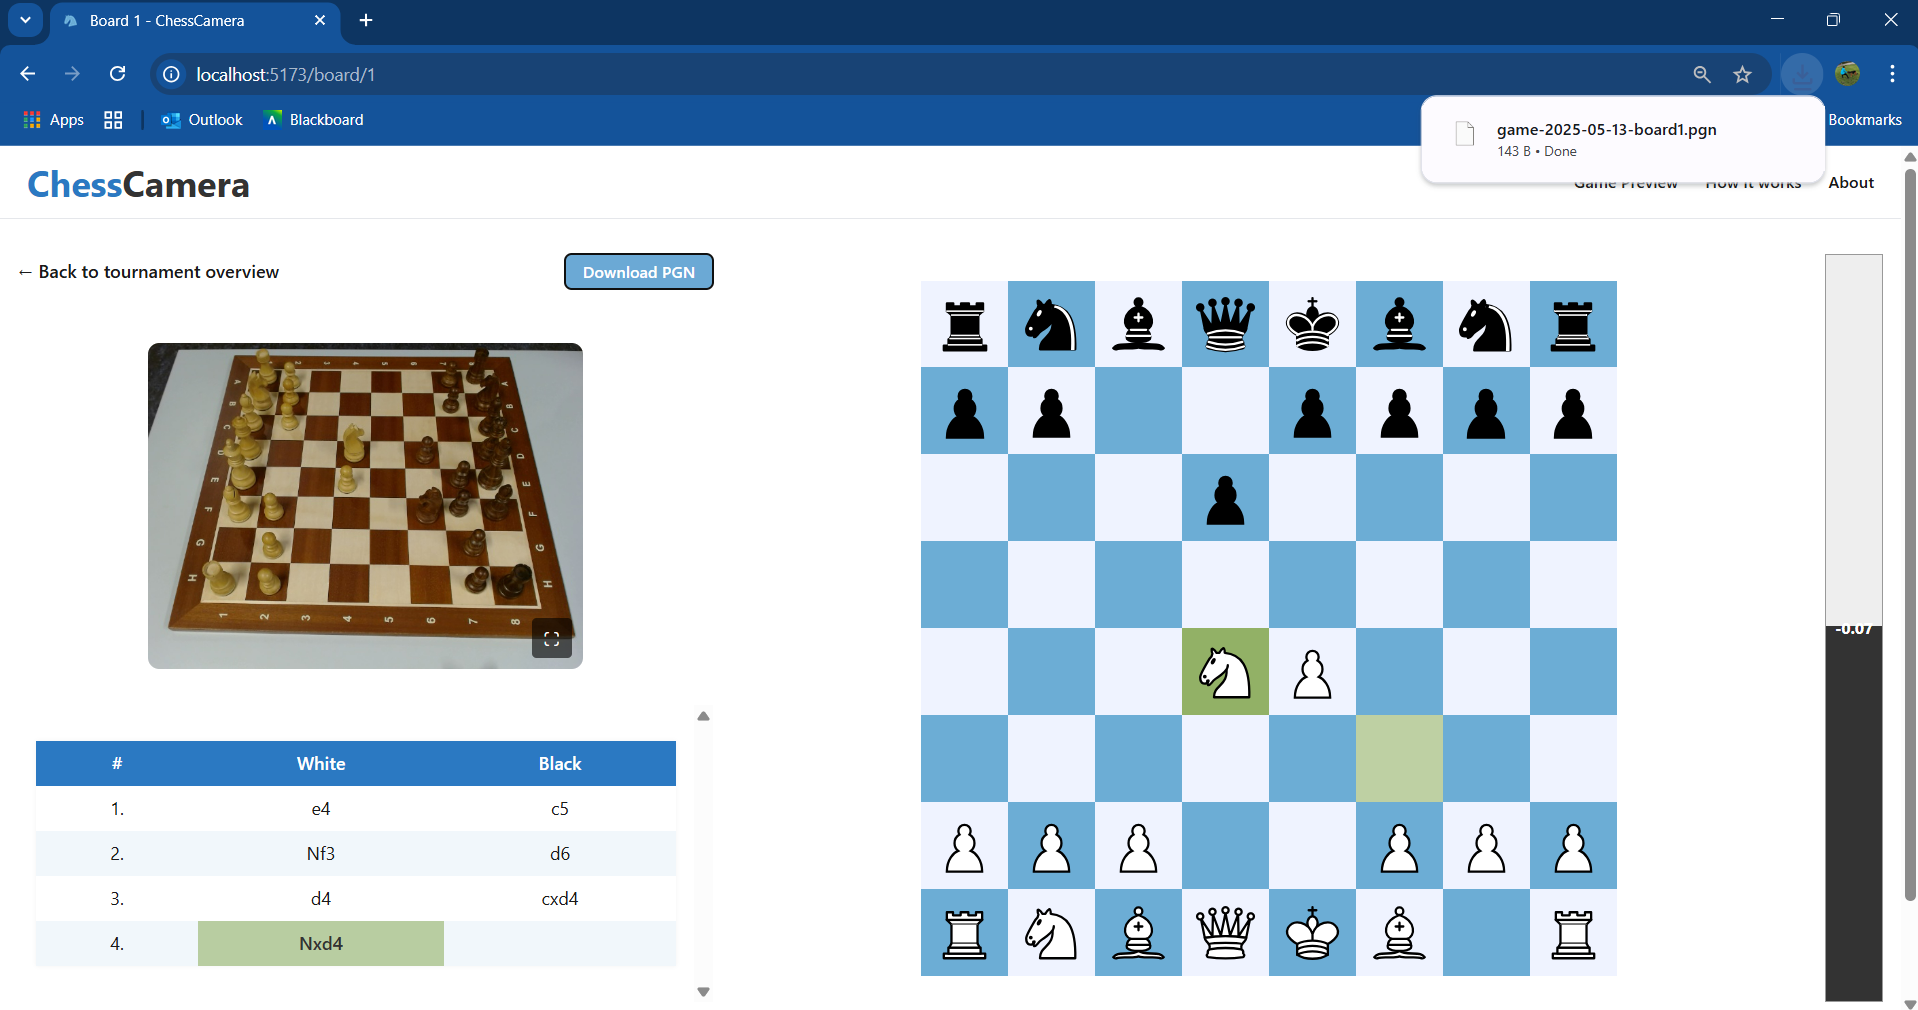
\includegraphics[width=0.75\linewidth]{figures/results/frontend/download-pgn/download-pgn.png}}\caption[Display of board view]{A demonstration of downloading a PGN file to a specific game}\label{fig:download-pgn} \end{figure}

The downloaded file includes a header with key information such as the tournament name, date, and player names, followed by the recorded moves. It also indicates whether the game is still in progress. When the game is completed, this field displays the result 1-0, 0-1, or $\frac{1}{2}$–$\frac{1}{2}$. Figure~\ref{fig:downloaded-pgn} shows an example of such a file. \\

\begin{figure}[h!] \centering \fbox{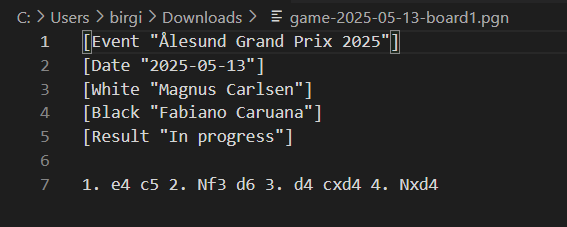
\includegraphics[width=0.75\linewidth]{figures/results/frontend/download-pgn/downloaded-pgn.png}}\caption[PGN file and metadata]{The downloaded PGN file to a specific game, opened in a code editor.}\label{fig:downloaded-pgn} \end{figure}

\section{Project Management}
\label{sec:results-project-management}
Although the project was initially structured according to the Scrum framework, its practical execution became more Scrum-inspired due to the absence of a dedicated Scrum Master and certain deviations from the full methodology. Each sprint began with a planning session in which tasks were selected from the product backlog based on priority and available team capacity. Sprint reviews were conducted at the end of each sprint to assess completed work and record outcomes. In addition, sprint retrospectives were held and documented, including reflections on workload distribution, communication challenges, and opportunities for process improvement. \\

Meeting routines were adapted according to team availability and project needs. Internal meetings were held as needed rather than on a fixed schedule, with most collaboration taking place informally during shared office hours. Nevertheless, short stand-up meetings were prioritized on a daily basis to maintain effective communication and ensure alignment. Biweekly meetings with the supervisor were consistently maintained, functioning as checkpoints for academic progress and clarification of requirements. Meetings with the product owner were arranged approximately once or twice per month and typically focused on feature validation, feedback, and adjustments. \\

GitHub was used consistently throughout the project for both task management and version control. Issues were linked to corresponding branches and categorized by type (e.g., feature, enhancement, documentation). All code changes were submitted via pull requests, and no changes were pushed directly to the main branch. Peer review was strictly enforced as part of the workflow, with every pull request reviewed by at least one team member before merging. \\

Tasks were assigned to individual team members and tracked using GitHub Issues. Issues were labeled and moved through the workflow stages: \textit{No Status}, \textit{To Do}, \textit{In Progress}, and \textit{Done}. This workflow was followed consistently for larger development tasks. However, some minor items, particularly quick fixes and small adjustments, were occasionally completed outside of the issue board during periods of intensive development, resulting in slightly reduced traceability for those changes.\\

In addition to manual code review, automated workflows were implemented using GitHub Actions to support continuous integration and reduce human error. One workflow was configured to run Python unit tests on every push, ensuring code stability throughout development. Another workflow was responsible for automatically updating LaTeX-based documentation by cloning the relevant repository and pushing changes after each update, as shown in Figure~\ref{fig:workflow-latex}. These pipelines contributed to improved reliability, automation of repetitive tasks, and early detection of breaking changes during development. \\

\begin{figure}[h!] \centering 
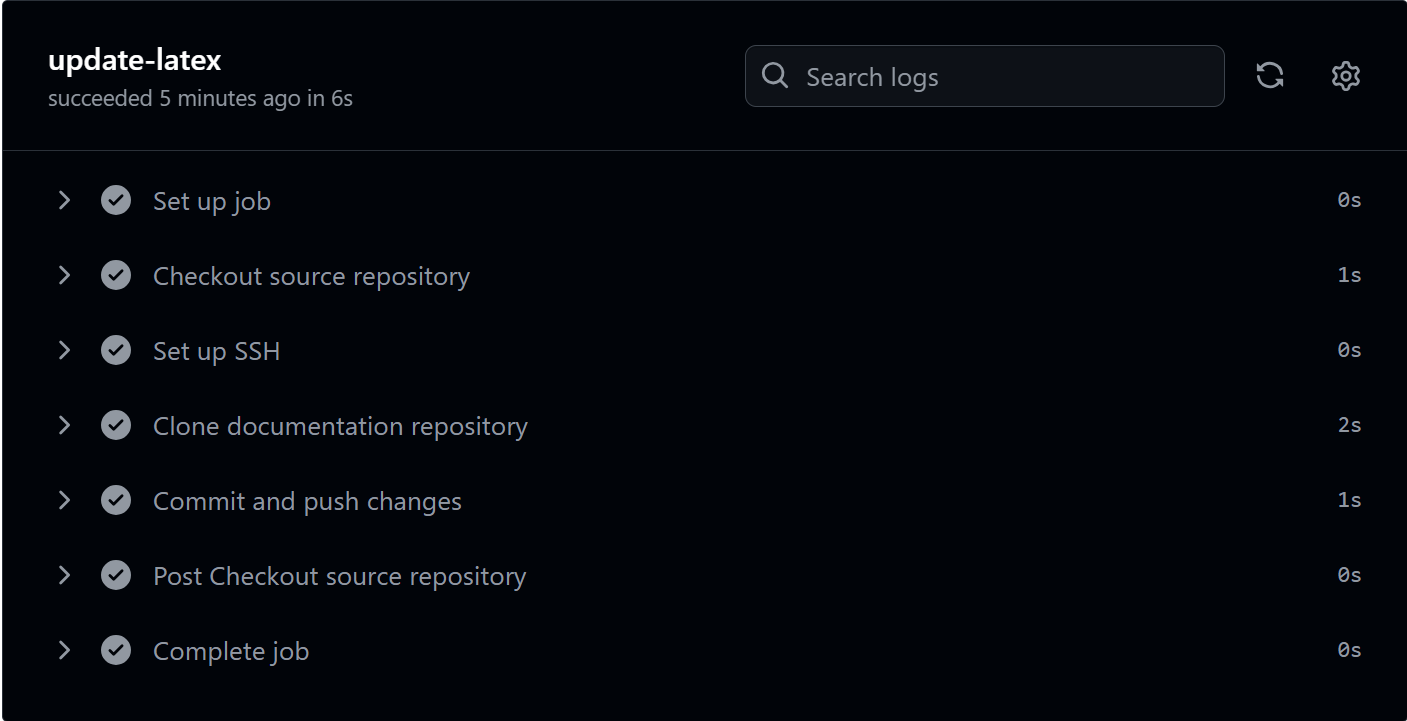
\includegraphics[width=0.75\linewidth]{figures/results/workflows/latex.png}\caption[Upload LaTeX workflow]{The workflow for update documentation with code.}\label{fig:workflow-latex} \end{figure}

\section{Technical Achievements}

\subsection{Architecture Overview}
\label{subsec:diagrams}

To provide a comprehensive understanding of the system architecture and interaction flow, several \gls{uml} diagrams were created. These diagrams model different aspects of the live chess game digitization system, from component interactions and activity flow to user roles and use cases.






\subsubsection*{Use-Case Diagram}
\label{subsubsec:use-case-diagram}

The use-case diagram, shown in Figure \ref{fig:use-case}, identifies the system’s main actors and the primary functionalities they interact with. Admins are responsible for hardware setup and initiating the game recording process. The system autonomously handles move detection, validation, and \gls{ui} updates. Users, on the otherhand, access the game remotely to spectate or download \gls{pgn} files. This diagram provides a clear overview of who interacts with the system and what capabilities are exposed, forming the basis for understanding system requirements and user expectations.

\begin{figure}[h!]
    \centering
    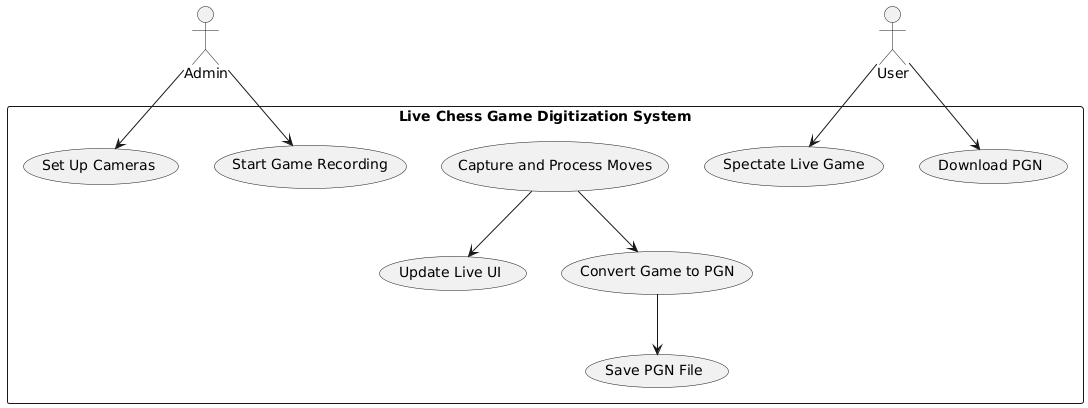
\includegraphics[width=0.75\linewidth]{figures/results/uml/use-case.png}
    \caption[Use-case diagram]{Use-case diagram outlining the system’s main actors and their interactions with key functionalities.}
    \label{fig:use-case}
\end{figure}  







\subsubsection*{Sequence Diagram}
\label{subsubsec:sequence-diagram}

The sequence diagram, shown in Figure \ref{fig:sequence}, illustrates the chronological flow of interactions between the system components and external actors. It begins with the admin initiating the game recording by setting up the camera, which captures and streams the board state to a local processing unit. This unit continuously detects and validates moves, updating the user interface accordingly. The diagram emphasizes the communication between hardware (camera and local machine) and the \gls{ui}, highlighting how physical chess games are digitized and broadcasted.


\begin{figure}[h!]
    \centering
    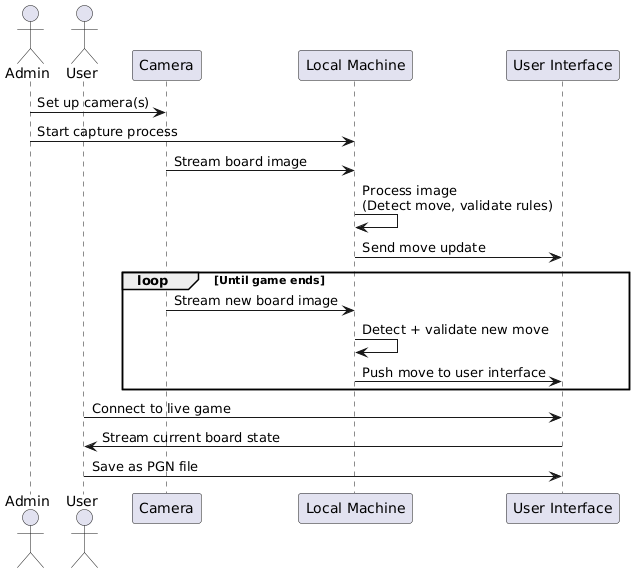
\includegraphics[width=0.75\linewidth]{figures/results/uml/sequence.png}
    \caption[Sequence diagram]{Sequence diagram showing the interaction flow between system components.}
    \label{fig:sequence}
\end{figure}












\subsubsection*{Class Diagram}

The class diagram in Figure \ref{fig:class} provides a high-level overview of the system’s object-oriented design, detailing the core components involved in the chess digitization process. The central class, \texttt{App}, acts as the main entry point for the application, orchestrating the initialization of system services and user interface components. It interacts with the \texttt{BoardFactory} to generate multiple \texttt{Board} instances, each representing a physical chessboard, and connects to GUI elements such as \texttt{ProgressBarTopLevel} and \texttt{BoardResetSelectorTopLevel}, which support board resets and progress tracking during gameplay. \\

Each \texttt{Board} object aggregates a \texttt{Camera} for video input and a \texttt{Detector} for move recognition using computer vision. It maintains a history of moves, manages WebSocket clients, and offers methods for validating and resetting board states. The \texttt{BoardService} class handles the overall control flow, managing boards, processing moves, and starting detector threads. Error handling is supported through a custom \texttt{CameraDoesNotExistError} exception. This structure ensures a clear separation of concerns, supporting modular development and maintainability across the data, control, and interface layers of the system.

\begin{figure}[h!]
\centering
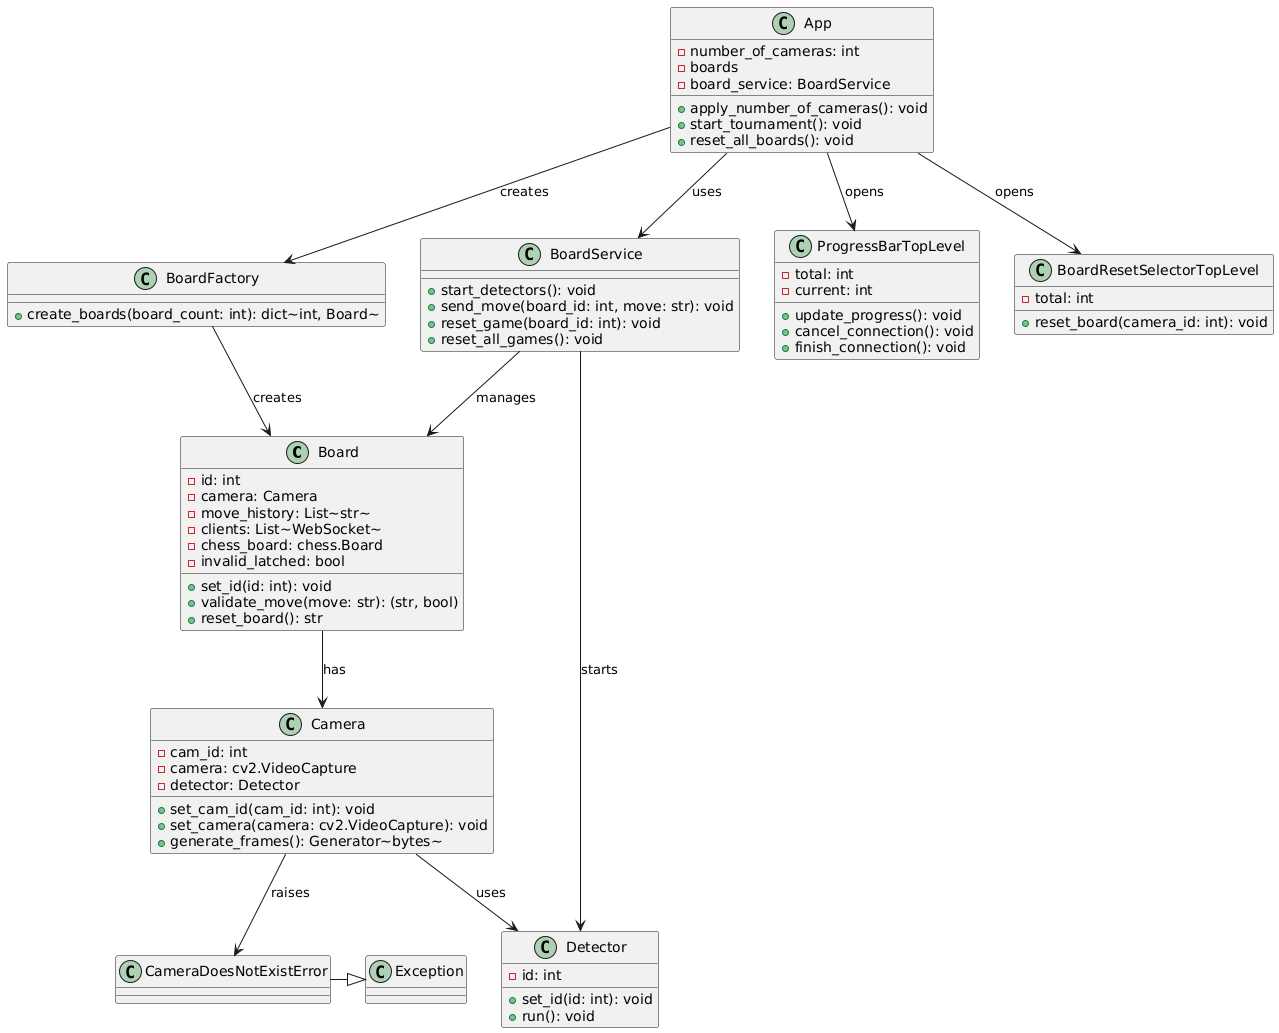
\includegraphics[width=0.75\linewidth]{figures/results//uml/class.png}
\caption[Class Diagram]{Class diagram of the chess digitization system.}
\label{fig:class}
\end{figure}






\subsubsection*{Package Diagram}

Figure \ref{fig:package-backend} illustrates the package structure of the backend system, organized around a modular architecture. The core logic resides in the \texttt{logic} package, which encapsulates domain-specific functionality such as board state detection, computer vision, mathematical operations, and supporting utilities. This modular breakdown, particularly in subpackages like \texttt{machine\_learning}, promotes separation of concerns and enhances reusability and testability. Alongside it, the \texttt{api} package handles external communication through submodules for data entities, service logic, and route definitions using FastAPI. Supporting components include static \texttt{resources} and the application entry point \texttt{main.py}, which binds the service and routing layers. This structure enables clean integration between backend services, data flow, and \gls{api} endpoints. \\

\begin{figure}[h!]
    \centering
    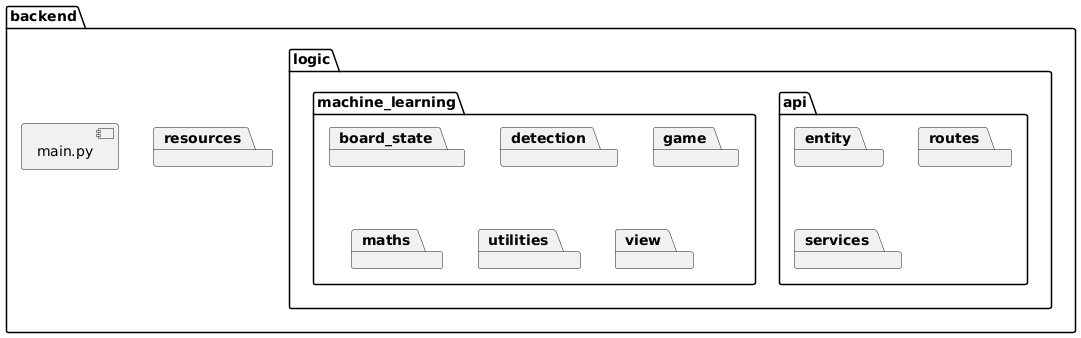
\includegraphics[width=\linewidth]{figures/results/uml/package-backend.png}
    \caption[Package Diagram for Backend]{Package Diagram for the backend package structure.}
    \label{fig:package-backend}
\end{figure}

On the frontend, shown in Figure \ref{fig:package-frontend}, the React application follows a conventional structure under the \texttt{src} directory. Key folders include \texttt{components} for reusable \gls{ui} elements like camera and board displays, \texttt{pages} for route-linked views, and \texttt{layouts} for defining common structural components across pages, such as headers or navigation bars. The \texttt{data} directory supports configuration or mock content during development. Outside \texttt{src}, the \texttt{public} folder holds static assets like \texttt{index.html}, while \texttt{App.tsx} and \texttt{index.css} define the main logic and styling. This organization supports maintainability and scalability by clearly separating visual components, logic, routing, and configuration.

\begin{figure}[h!]
    \centering
    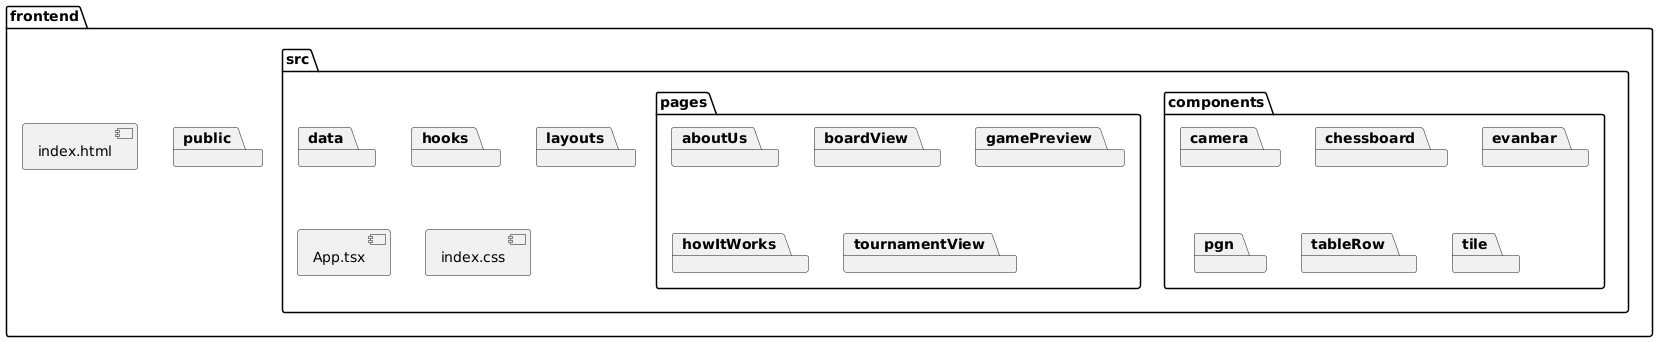
\includegraphics[width=\linewidth]{figures/results/uml/package-frontend.png}
    \caption[Package Diagram for Frontend]{Package Diagram for the frontend package structure.}
    \label{fig:package-frontend}
\end{figure}








\begin{figure}[H]
    \subsubsection*{Activity Diagram}
    \label{subsubsec:activity-diagram}
    
    \centering
    \begin{minipage}[t]{0.5\textwidth}
        \vspace{0pt}
        The activity diagram, shown in Figure \ref{fig:activity}, provides a high-level overview of the operational workflow during a chess game session. It models the continuous loop of capturing board states, detecting and validating moves, and updating the game state until the game ends. If a move is invalid, the system flags it but does not terminate the session. Once the game concludes, it is converted into a standard \gls{pgn} format. This diagram emphasizes the logical flow and decision-making process, reflecting the system’s role in automating and maintaining the integrity of live digitization.
    \end{minipage}
    \hfill
    \begin{minipage}[t]{0.45\textwidth}
        \vspace{0pt}
        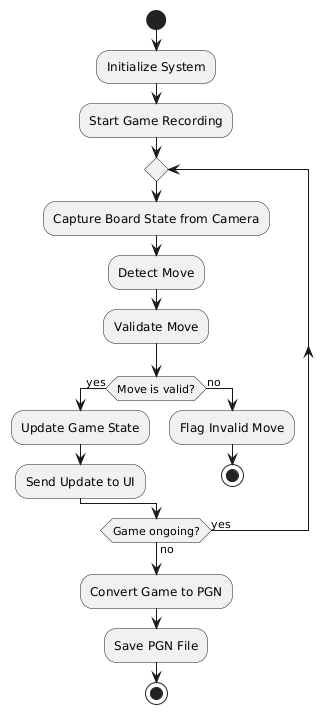
\includegraphics[width=\linewidth]{figures/results/uml/activity-2.png}
        \caption[Activity Diagram]{Activity diagram illustrating the system workflow.}
        \label{fig:activity}
    \end{minipage}
\end{figure}







\begin{figure}[H]
    \subsubsection*{State Machine Diagram}
    \label{subsubsec:state-machine-diagram}

    \centering
    \begin{minipage}[t]{0.5\textwidth}
        Figure \ref{fig:state-machine} illustrates the state machine governing move detection and validation in the chess digitization system. The process begins in a waiting state, idling until a physical move is made. It then enters the detection phase, where the system captures and analyzes images using a machine learning model to identify the move. \\

        Once detected, the system transitions to a validation phase, where the move is checked for legality. Valid moves are displayed on the \gls{ui} and the system returns to its waiting state. Invalid moves lead to process termination. This diagram emphasizes the reactive, event-driven flow of the system, moving from detection to validation and feedback in response to user actions.
    \end{minipage}
    \hfill
    \begin{minipage}[t]{0.45\textwidth}
        \vspace{0pt}
        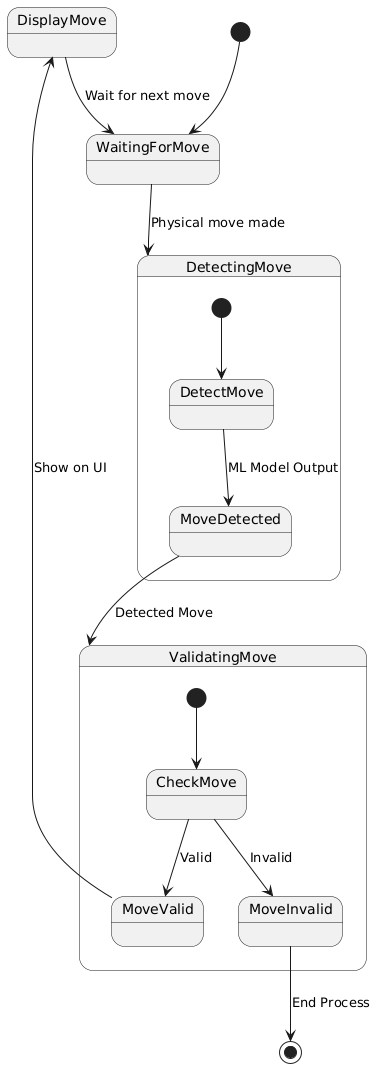
\includegraphics[width=\linewidth]{figures/results/uml/state-machine.png}
        \caption[State Machine Diagram]{State machine for move detection and validation.}
        \label{fig:state-machine}
    \end{minipage}
\end{figure}










\section{Testing and Quality Assurance}

\subsection{Machine Learning Model}
\label{machine-learning-test}

As described in Section~\ref{subsec:model-testing}, the model was evaluated using 100 games. Table~\ref{tab:accuracy-total} presents the overall move detection accuracy, both in total and broken down by piece type and color. The model achieved an overall accuracy of 90.6\%, successfully detecting 936 out of 1033 moves. Pawns had the highest detection rates, with over 98\% accuracy for both colors. In contrast, the model struggled particularly with black rooks with only 23.8\% accuracy.

\begin{table}[htbp]
\centering
\caption{Move detection accuracy total}
\label{tab:accuracy-total}
\begin{tabular}{lccc}
\toprule
\textbf{Category} & \textbf{OTB Moves} & \textbf{Successful Moves} & \textbf{Accuracy (\%)} \\
\midrule
\textbf{White Pieces} & & & \\
\hspace{1em}Pawn  & 244 & 242 & 99.2\% \\
\hspace{1em}Knight & 128 & 117 & 91.4\% \\
\hspace{1em}Bishop & 74  & 54  & 73.0\% \\
\hspace{1em}Rook   & 29  & 25  & 86.2\% \\
\hspace{1em}Queen  & 42  & 40  & 95.2\% \\
\hspace{1em}King   & 16  & 8   & 50.0\% \\
\midrule
\textbf{Black Pieces} & & & \\
\hspace{1em}Pawn  & 247 & 243 & 98.4\% \\
\hspace{1em}Knight & 78  & 75  & 96.2\% \\
\hspace{1em}Bishop & 65  & 47  & 72.3\% \\
\hspace{1em}Rook   & 21  & 5   & 23.8\% \\
\hspace{1em}Queen  & 84  & 76  & 90.5\% \\
\hspace{1em}King   & 5   & 4   & 80.0\% \\
\midrule
\textbf{Total} & 1033 & 936 & 90.6\% \\
\bottomrule
\end{tabular}
\end{table}


Table \ref{tab:board-type-accuracy} compares the success rates between the two physical board types used during testing. The wooden board slightly outperformed the plastic board, with a 91.2\% success rate compared to 89.9\%. This marginal difference may indicate a slightly more stable detection environment on the wooden surface. \\


\begin{table}[htbp]
\centering
\caption[Move detection accuracy board type]{Summary of total moves and success rate by board type}
\label{tab:board-type-accuracy}
\begin{tabular}{lccc}
\toprule
\textbf{Board Type} & \textbf{Total Moves} & \textbf{Total Successful Moves} & \textbf{Success Rate (\%)} \\
\midrule
Plastic & 475 & 427 & 89.9\% \\
Wooden  & 558 & 509 & 91.2\% \\
\bottomrule
\end{tabular}
\end{table}


Figure \ref{fig:move-failures} shows the number of failed games (i.e., games where detection failed) grouped by the move number at which failure occurred. Bars are color-coded by board type. The majority of failures occurred within the first five moves, particularly at moves 2, 4, and 5. This trend suggests that the early game presents the greatest challenge for detection, potentially due to rapid development or ambiguity in piece positions. Notably, failures after move 9 were rare. \\


\begin{figure}[h!]
\centering
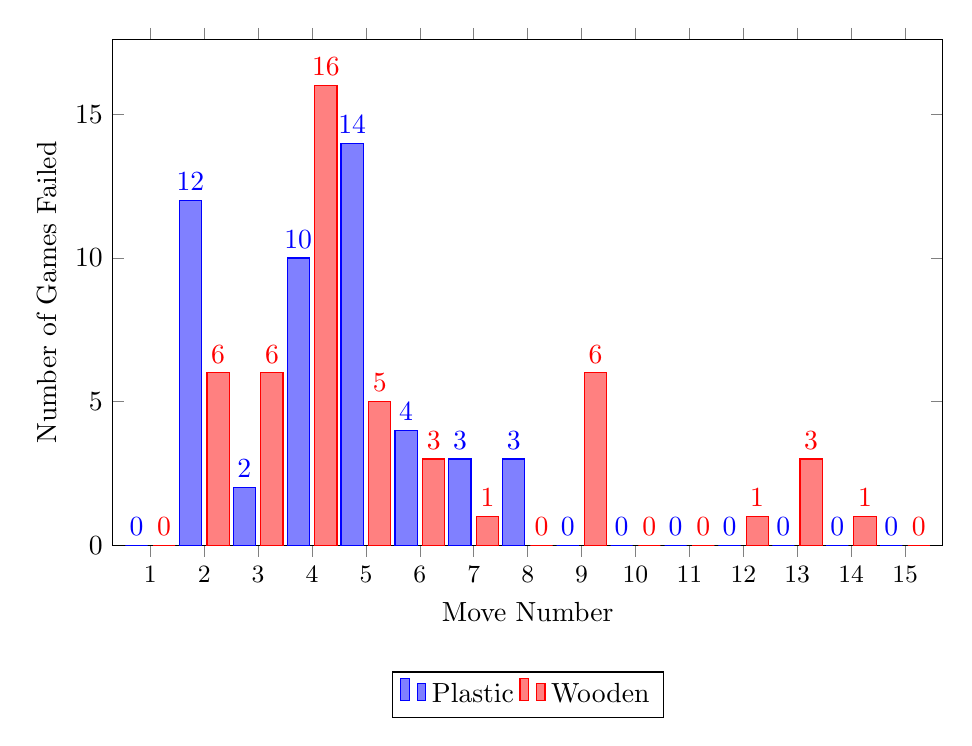
\begin{tikzpicture}
\begin{axis}[
    ybar,
    bar width=8pt,
    width=\textwidth,
    height=8cm,
    enlarge x limits=0.05,
    ymin=0,
    ylabel={Number of Games Failed},
    xlabel={Move Number},
    xtick={1,...,15},
    xticklabels={1,2,3,4,5,6,7,8,9,10,11,12,13,14,15},
    x tick label style={rotate=0, anchor=north, font=\small},
    legend style={at={(0.5,-0.25)}, anchor=north, legend columns=-1},
    nodes near coords,
    symbolic x coords={1,2,3,4,5,6,7,8,9,10,11,12,13,14,15},
    xticklabel style={font=\small},
]
\addplot+[style={fill=blue!50}] coordinates {
    (1,0) (2,12) (3,2) (4,10) (5,14) (6,4) (7,3) (8,3) (9,0)
    (10,0) (11,0) (12,0) (13,0) (14,0) (15,0)
};
\addplot+[style={fill=red!50}] coordinates {
    (1,0) (2,6) (3,6) (4,16) (5,5) (6,3) (7,1) (8,0) (9,6)
    (10,0) (11,0) (12,1) (13,3) (14,1) (15,0)
};
\legend{Plastic, Wooden}
\end{axis}
\end{tikzpicture}
\caption[Detection failures per move number]{Number of failed games per move number across plastic and wooden boards.}
\label{fig:move-failures}
\end{figure}


Table \ref{tab:different-errors} categorizes the types of detection failures for each board type. The majority of failures were due to a complete lack of detection within the allotted time window. Incorrect detections (the model detecting a move but interpreting it wrongly) were less frequent but more common on the wooden board, accounting for 8 out of 48 failures, compared to just 1 on the plastic board.  \\

\begin{table}[htbp]
\centering
\caption[Different detection errors]{Frequencies of Different Detection Errors}
\label{tab:different-errors}
\begin{tabular}{lccc}
\toprule
\textbf{Board Type} & \textbf{Total Failures} & \textbf{No Detection} & \textbf{Incorrect Detection} \\
\midrule
Plastic & 48 & 47 & 1 \\
Wooden & 48 & 40 & 8 \\
\midrule
\textbf{Total} & 96 & 87 & 9 \\
\bottomrule
\end{tabular}
\end{table}

For a detailed breakdown of the chess games, including the sequences of moves, failure points, and detection statistics for each board type, see Appendix FILL IN.

\subsection{API}

\subsection{Wireframe}
\label{subsec:wireframe-results}

A total of eight individuals participated in the wireframe usability test, excluding project developers and stakeholders. While the sample size was limited, participants were intentionally selected to represent a broad range of ages, technical backgrounds, and familiarity with chess. \\

Overall, the feedback was generally positive. Participants were asked to rate their satisfaction on a 1–5 Likert scale. Figure \ref{fig:wireframe-test-results} shows the distribution of the ratings. The average scores from the feedback form were as follows:

\begin{itemize}
    \item The \textbf{overall user experience} received an average rating of \textbf{4.63} out of 5.
    \item The \textbf{Tournament View page} received the highest average rating of \textbf{4.75}.
    \item The \textbf{Board View page} received a slightly lower average rating of \textbf{4.38}.
\end{itemize}

Participants commented that the interface was easy to navigate and that the layout felt intuitive. The Tournament View, in particular, was praised for its clarity and structure. Several testers without prior experience using chess-related software indicated that the interface felt approachable and visually clear. \\

However, participants also suggested a few areas for improvement:

\begin{itemize}
    \item Adding a full-screen function for the video feed.
    \item Enhancing the visual design of some \gls{ui} elements for improved aesthetics.
    \item Supporting multiple languages for users who do not speak English.
\end{itemize}

While these findings are based on a small participant group, they offer early indications that the interface is both accessible and functional for a wide range of users. These insights will guide further development and refinement of the user interface.

\begin{figure}[h!]
\centering
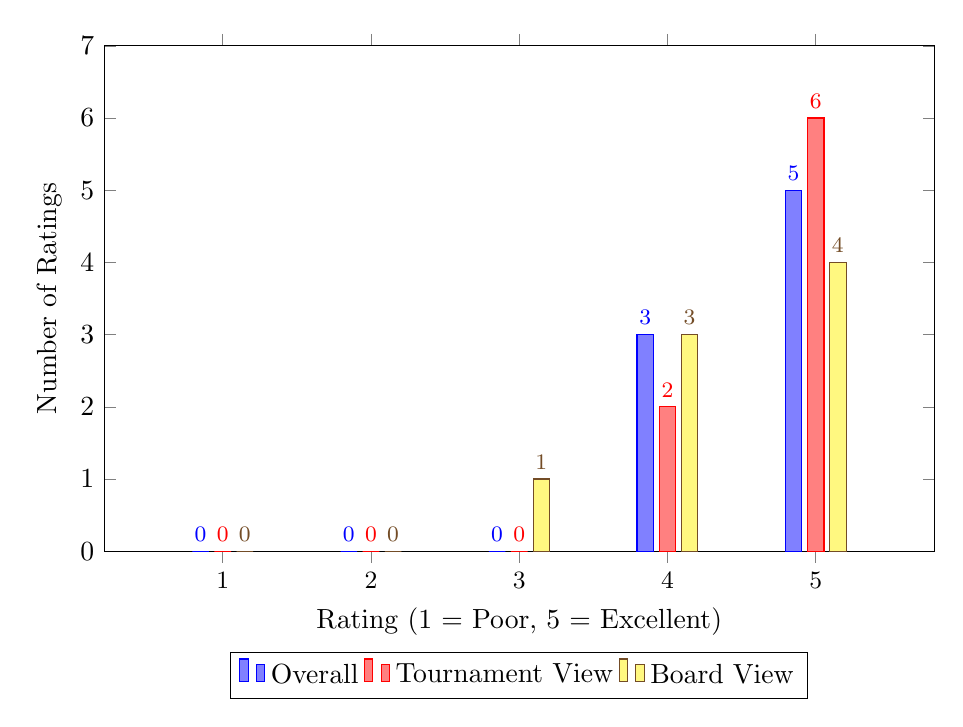
\begin{tikzpicture}
\begin{axis}[
    ybar,
    bar width=6pt,
    width=\textwidth,
    height=8cm,
    enlarge x limits=0.2,
    ymin=0,
    ymax=7,
    ylabel={Number of Ratings},
    xlabel={Rating (1 = Poor, 5 = Excellent)},
    symbolic x coords={1,2,3,4,5},
    xtick=data,
    x tick label style={rotate=0, anchor=north, font=\small},
    legend style={
        at={(0.5,-0.2)},
        anchor=north,
        legend columns=3
    },
    nodes near coords,
    nodes near coords style={font=\footnotesize},
    every node near coord/.append style={
        /pgf/number format/.cd,
        fixed,
        precision=0,
        /tikz/ifthenelse/.code={
            \ifnum\pgfplotspointmeta=0
                \pgfkeys{/pgfplots/disable node}
            \fi
        }
    }
]
\addplot+[style={fill=blue!50}] coordinates {
    (1,0) (2,0) (3,0) (4,3) (5,5)
};
\addplot+[style={fill=red!50}] coordinates {
    (1,0) (2,0) (3,0) (4,2) (5,6)
};
\addplot+[style={fill=yellow!50}] coordinates {
    (1,0) (2,0) (3,1) (4,3) (5,4)
};
\legend{Overall, Tournament View, Board View}
\end{axis}
\end{tikzpicture}
\caption[Satisfaction rating distribution]{Distribution of satisfaction ratings from participants across different interface views.}
\label{fig:wireframe-test-results}
\end{figure}



\subsection{Color Palette}
\label{subsec:results-color-palette}
Voting revealed a mix of preferences: some participants favored the light mode from palette \#08 and the dark mode from palette \#07, while others selected the board design from palette \#05 or the move-highlighting style from palette \#14. \\

Rather than selecting a single predefined palette, the final color scheme was assembled by combining the most highly rated elements across the top-voted variations, yielding a more tailored, user-informed visual design. Figure \ref{fig:color-palette-results} shows the distribution of votes across all tested palettes; the full set of prototypes appears in Appendix \ref{app:color-palettes}.

\begin{figure}[h!]
\centering
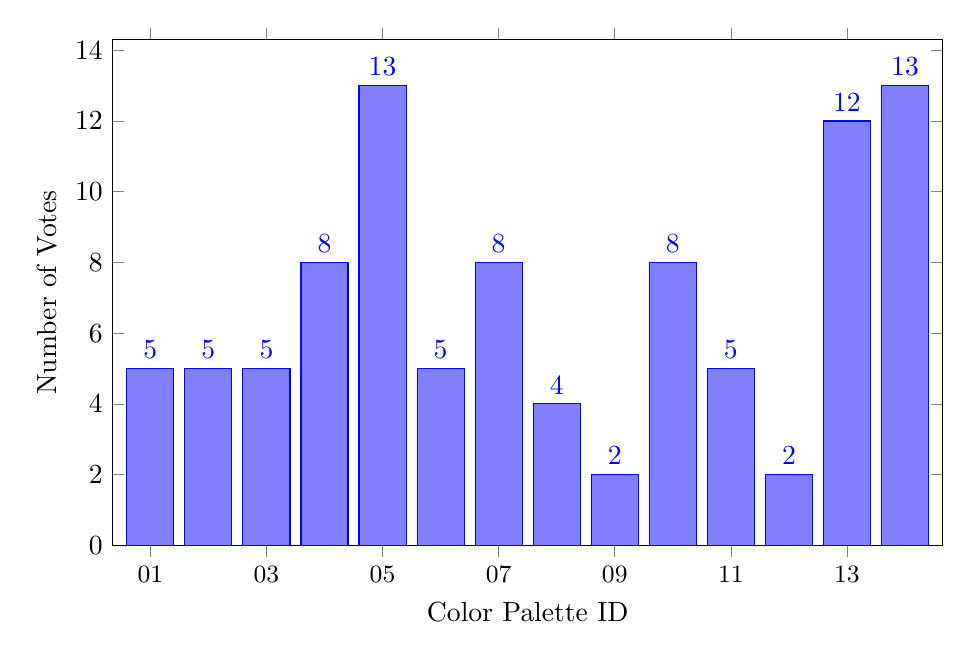
\begin{tikzpicture}
\begin{axis}[
    ybar,
    bar width=17pt,
    width=\textwidth,
    height=8cm,
    enlarge x limits=0.05,
    ymin=0,
    ylabel={Number of Votes},
    xlabel={Color Palette ID},
    xticklabels={01,02,03,04,05,06,07,08,09,10,11,12,13,14},
    x tick label style={rotate=0, anchor=north, font=\small},
    nodes near coords,
    symbolic x coords={01,02,03,04,05,06,07,08,09,10,11,12,13,14},
    xticklabel style={font=\small},
]
\addplot+[style={fill=blue!50}] coordinates {
    (01, 5) (02, 5) (03, 5) (04, 8) (05, 13) (06, 5) (07, 8) (08, 4) (09, 2) (10, 8) (11, 5) (12, 2) (13, 12) (14, 13)
};
\end{axis}
\end{tikzpicture}
\caption[Votes per color palette]{Distribution of Votes Across Different Color Palettes}
\label{fig:color-palette-results}
\end{figure}
\cleardoublepage

\chapter{Discussion}

\begin{center}
    \textit{The results are analyzed and discussed in this chapter. It explores the implications of the findings, identifies limitations, and suggests potential areas for future improvement.}
\end{center}

\section{Overview of Delivered Product}
The delivered product functions as intended and meets all defined requirements. It allows players to conduct \gls{otb} chess games using a traditional physical board, while each move is automatically detected, validated, and stored digitally in \gls{pgn} format. These \gls{pgn} files can be accessed in real time through the frontend interface, enabling both live viewing and post-game analysis. \\

The core functionality of the system has proven to be reliable across different test scenarios, see Section \ref{machine-learning-test}. Players are able to engage with the game naturally, without needing to alter their usual playing behavior or interact directly with the system during gameplay. The seamless digitization process provides a user-friendly experience, especially for tournament organizers or spectators who wish to follow games live. \\

Despite this, a minor delay is present between the moment a physical move is made and its appearance on the digital board. This latency is primarily caused by the time required for image capture, model inference, and subsequent processing. While the delay does not significantly impact usability, it could be minimized through further optimization of the machine learning models or by deploying the system on more powerful hardware. \\

Move validation is handled through a three-step process to ensure both accuracy and legality of each detected move. The machine learning model first detects changes on the board, followed by backend validation using a chess engine that checks the move against the current game state. Finally, the frontend performs an additional check before updating the display. If an illegal move is identified at any point, the system stops further updates to prevent errors or corrupted game data. In line with the product owner's request, the system includes no extra error handling or user notifications. It is intended solely as a display tool for passive observation and live broadcasting, not as an active referee. This approach keeps the interface simple while preserving reliable and consistent game visualization.

\section{Machine Learning Model}

The overall move accuracy across all games was 90.6\%. Performance between board types was similar, with slightly better detection rates on the wooden board (91.2\%) compared to the plastic board (89.9\%), as shown in Table \ref{tab:board-type-accuracy}. This minor difference may be attributed to the higher visual contrast between the wooden pieces and the board surface, than the black and white pieces for the plastic board. \\

While the ChessCam models used in this project demonstrate high precision and recall under ideal conditions (Section \ref{chesscam-metrics}), our real-world move detection accuracy of 90.6\% is naturally lower. This is expected, as full move detection in physical games involves not just accurate identification of pieces and board geometry, but also handling lighting variations, ambiguous moves (castling) and general noise. Thus, the ChessCam metrics serve more as an upper bound, while our results reflect the practical challenges of real-time, physical chess move recognition. \\

One consistent source of error was tied to specific move numbers within certain openings. In some test sets, all 10 games of a particular opening failed at the same move, suggesting that specific board states challenge the model. This caused some piece types, especially the black rook, to receive unusually low scores (23.8\%). Since black rooks had relatively few moves overall and repeatedly failed at the same point in the games, their scores were artificially suppressed. \\

Another common issue involved the model misclassifying castling moves. The model selects the move with the highest predicted probability, but during castling, it often assigned a higher probability to the rook’s move from its original square rather than to the king’s two-square move. As a result, castling was frequently mistaken for a rook move. Of the 9 total misclassifications, 8 were caused by this specific error. One potential solution is to delay the rook’s movement by moving the king two squares first. This would give the model only one valid move to detect, reducing the likelihood of misclassification. \\

There was also observed reduced accuracy along the edges of the board, affecting both piece detection and the localization of square centers. Several factors contribute to this. The board-warping algorithm depends heavily on precise corner detection, which is more error-prone near the edges. The steep camera angle causes pieces closer to the camera to appear larger and obscure important details. Meanwhile, pieces farther away appear smaller and are more difficult to detect. Figure \ref{fig:bbox-centers-incorrect} illustrates this issue, showing bounding boxes near the edges that are frequently misaligned and square centers that are noticeably offset. In contrast, detection accuracy and alignment improve significantly toward the center of the board.

Another limitation observed was the model's handling of the en passant. Currently, the model does not support recognition of en passant moves. When the board state includes the possibility for such a move, the model fails to handle it correctly and crashes.


\begin{figure}[h!]
    \centering
    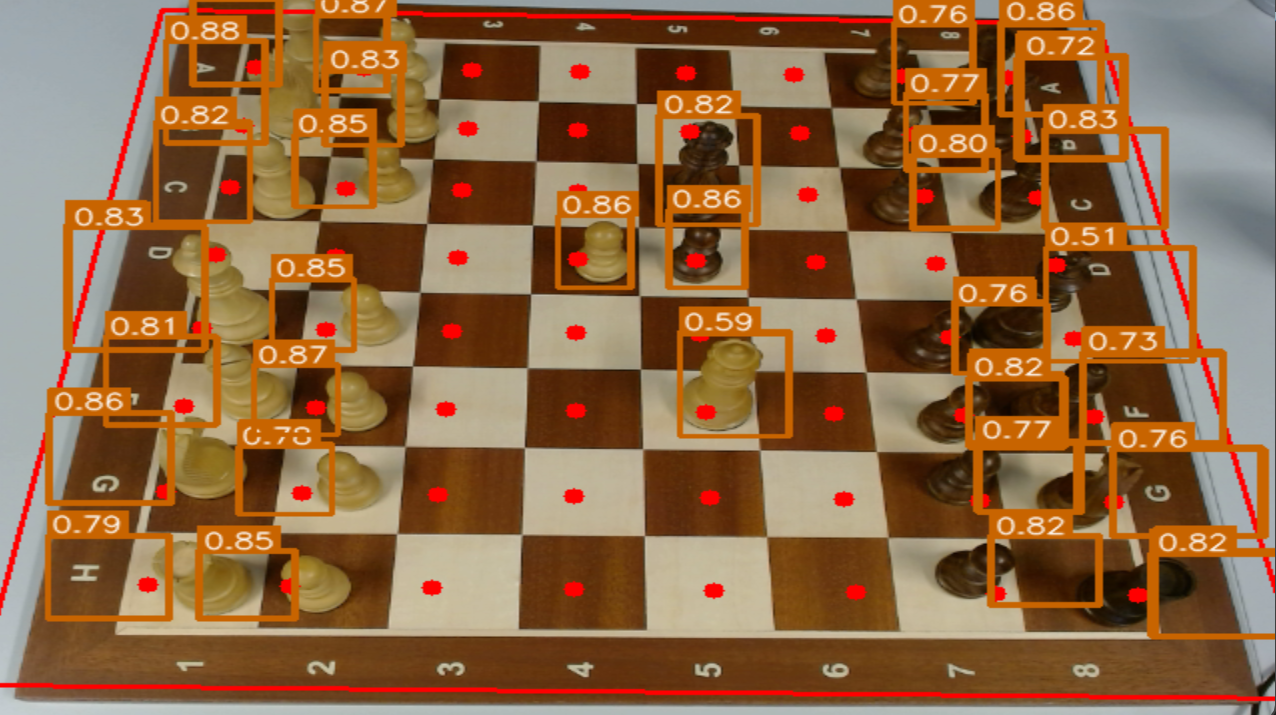
\includegraphics[width=0.75\linewidth]{figures/discussion/bbox-centers-incorrect.png}
    \caption[Bounding box and square center misalignment]{Bounding boxes and square centers overlaid on a physical chessboard. Boxes and square centers near the edges are misaligned.}
    \label{fig:bbox-centers-incorrect}
\end{figure}


\section{API}
The system is based on a client-server architecture, in which the frontend operates as the client and communicates with a centralized backend server. The backend is responsible for core functionalities such as data processing and move validation. This architectural separation promotes scalability and maintainability by allowing the frontend and backend to evolve independently while maintaining efficient communication. \\

To facilitate real-time interaction between these components, the system primarily employs the WebSocket protocol. In contrast to traditional \gls{http}, which operates on a request-response model, WebSocket establishes a persistent, full-duplex connection. This allows both the client and server to continuously exchange data without the overhead of repeated \gls{http} requests. As a result, the system significantly reduces latency and network load, ensuring that the frontend is promptly updated whenever new moves are processed by the backend.

\section{Frontend}
The frontend was developed based on the initial wireframes but was modified throughout the project in response to feedback from the supervisor, product owner, and user testing. Despite these adjustments, the core components and functionality remained consistent with the original design.

\subsection{Game preview}
The Game Preview page was not part of the initial wireframe, as described in Section \ref{subsec:wireframe}. However, following a suggestion from the product owner, this feature was added to provide a better overall overview of all ongoing games. One scenario for this functionality is when a spectator wishes to follow multiple games simultaneously. \\

Since the application architecture was already based on individual chessboard instances, implementing this feature was relatively straightforward. By reusing existing chessboard components identified by unique IDs, the Game Preview page was able to display all active games dynamically. Only minor code modifications were necessary to make the component more flexible and support this functionality.

\subsection{Download PGN file}
One project requirement was to digitize chess games into \gls{pgn} files, enabling players and spectators to download and analyze them using external tools such as lichess’ analysis feature. As described in Section \ref{subsec:results-frontend}, the application provides access to PGN files containing technical metadata. \\

The \gls{pgn} format is widely supported, and tools such as lichess can interpret both the complete file or just the move list. This flexibility allows users to gain insights into various aspects of the game, such as identifying the opening played, evaluating move accuracy, and understanding the overall game progression. Figure \ref{fig:downloaded-pgn-analysis} shows how the downloaded \gls{pgn} can be used in an external analysis tool. \\

\begin{figure}[h!] \centering \fbox{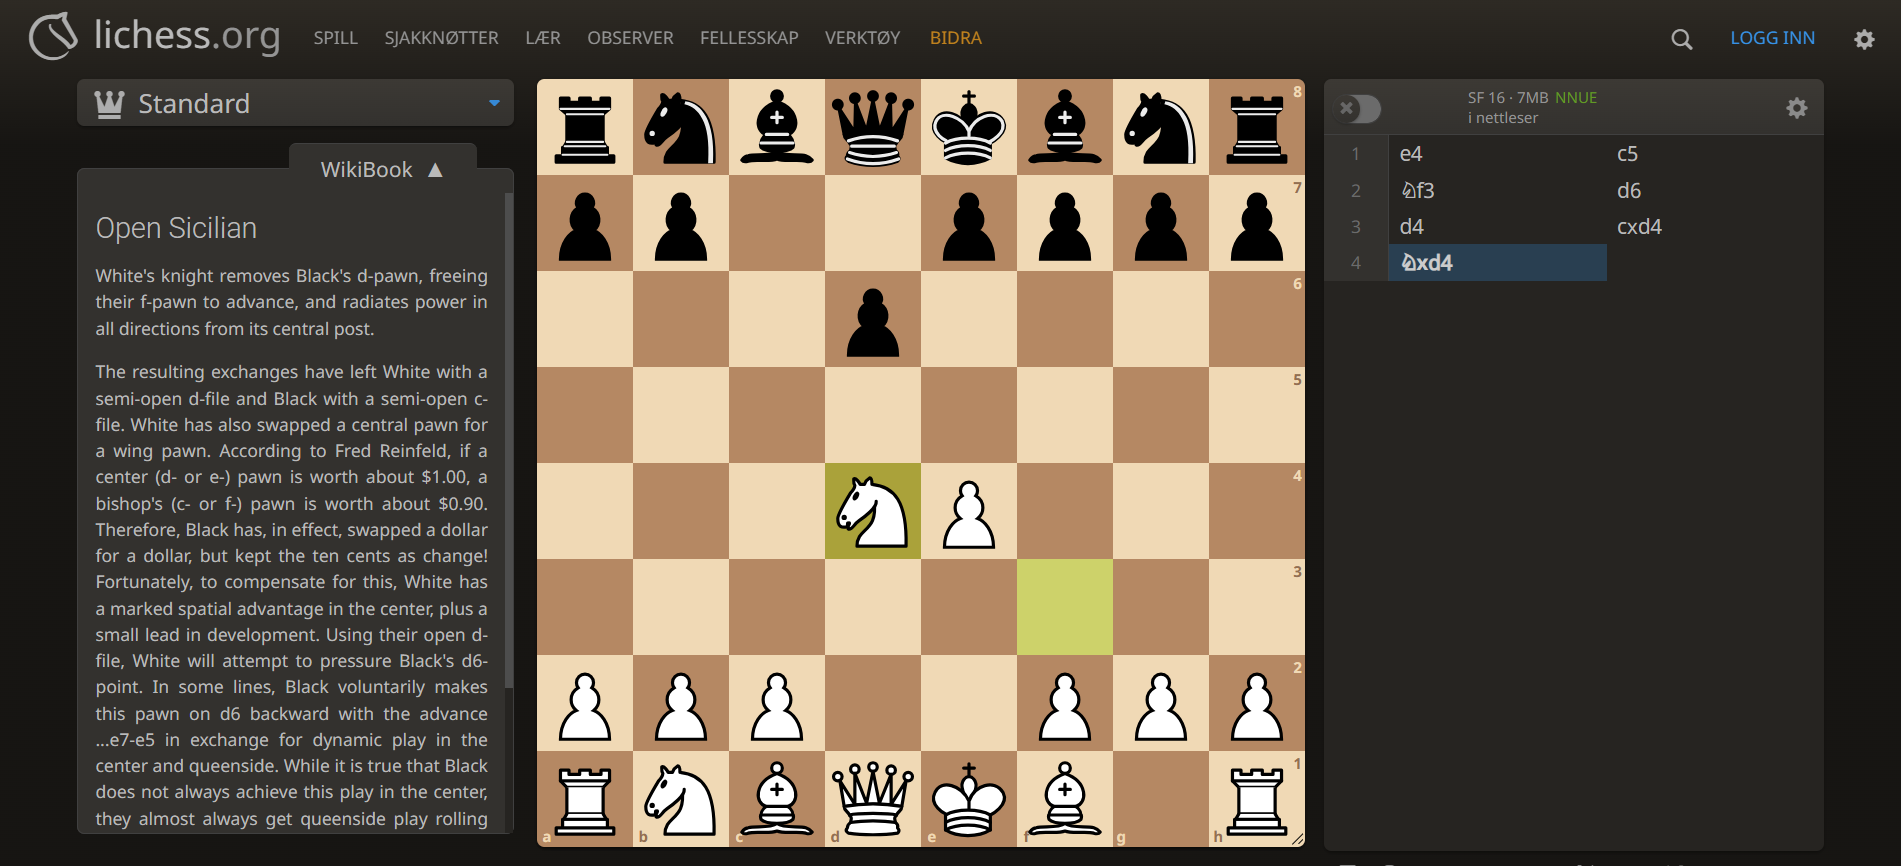
\includegraphics[width=0.75\linewidth]{figures/results/frontend/download-pgn/lichess-analysis.png}}\caption[Lichess analysis tool]{A demonstration of importing a PGN file into Lichess' analysis tool}\label{fig:downloaded-pgn-analysis} \end{figure}

By enabling \gls{pgn} downloads, the system provides users with a convenient way to review games and improve their understanding of chess. Instead of building a custom in-app analysis feature, this solution leverages existing, well-established services that offer robust and detailed feedback. This decision reduces development complexity while still providing users with valuable insights. \\

However, one limitation is that users must leave the application to analyze the game, which can disrupt the user experience. Despite this, integrating \gls{pgn} downloads remains a practical and effective solution, offering immediate access to game data without requiring additional implementation of complex analytical features.

\subsection{Lighthouse Tests}
The frontend application was developed based on wireframes, team discussions, and user testing. To evaluate the quality of the user interface, Lighthouse tests were conducted on every page, with particular focus on the accessibility score. \\

Initial accessibility scores ranged from 80 to 90 across the various pages. To improve these scores, several adjustments were required, primarily involving color contrast. As shown in \ref{subsec:results-color-palette}, a specific color palette was selected for the application. However, issues were identified with the contrast between the primary blue color and the white background in light mode, as well as between the secondary blue (used for buttons) and the black background in dark mode. \\

To address these issues, slightly modified color variants were chosen for each theme. This led to the adoption of a more customized color palette for both light and dark modes. As a result, the application now achieves a 100 accessibility scores throughout all pages, with both light and dark mode. 

\section{Project management}
\label{sec:discussion-project-management}

The application of a \gls{scrum} inspired methodology proved to be an effective project management strategy, particularly given the composition and size of the team. While the team followed core \gls{scrum} practices such as sprint planning, reviews, and retrospectives, the absence of a dedicated \gls{scrum} Master led to a more lightweight and adaptive implementation. Responsibilities typically associated with the \gls{scrum} Master role, such as facilitating meetings and managing the sprint process, were informally distributed among team members. This approach enabled greater flexibility and autonomy, which aligned well with the needs of a smaller team. \\

The communication within the team functioned efficiently throughout the project. Daily in-person collaboration during office hours allowed for rapid feedback, informal stand-ups, and immediate resolution of issues. The accessibility of all team members facilitated a high degree of responsiveness, reducing reliance on scheduled meetings and improving overall coordination.\\

Version control and task management were handled using Git, which provided a robust framework for organizing and reviewing code. Each task was implemented in a dedicated branch and linked to a corresponding GitHub issue. All changes were integrated into the main branch exclusively through pull requests, with peer review enforced for every contribution. This workflow contributed to maintaining code quality, minimizing integration issues, and ensuring transparency in the development process. \\

GitHub Actions was used to automate the development process, including running Python unit tests and updating LaTeX documentation. This improved efficiency and helped catch issues early. However, the test workflow consistently failed in the CI environment due to its dependence on camera hardware (see Figure \ref{fig:workflow-test}). Since this hardware was unavailable during automated runs, the failures were expected and did not impact the final delivery. This highlighted the need to separate hardware-dependent tests from those suitable for standard test environments.\\

\begin{figure}[h!] \centering 
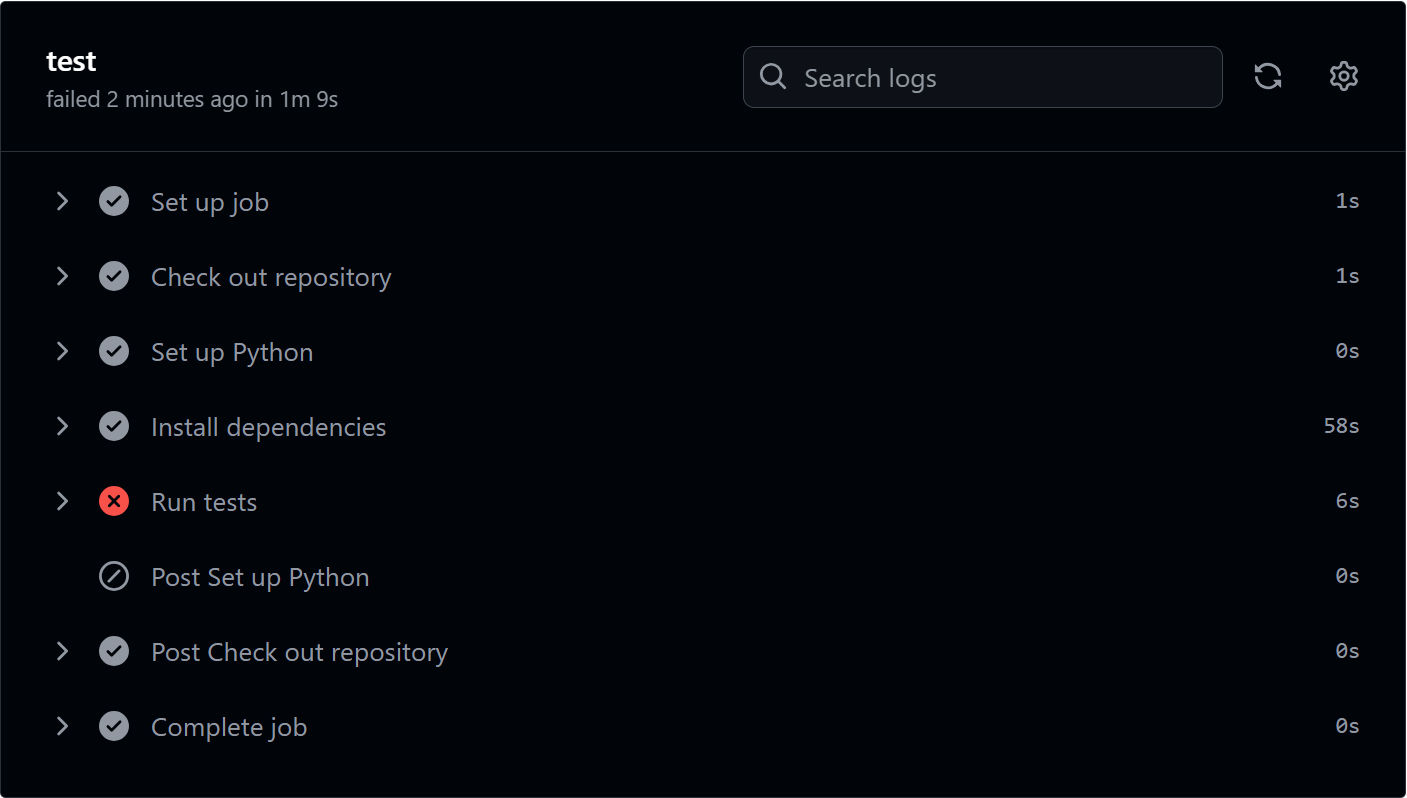
\includegraphics[width=0.75\linewidth]{figures/results/workflows/tests.png}\caption[Python tests workflow]{The workflow for Python unit tests}\label{fig:workflow-test} \end{figure}

Overall, the project management approach successfully balanced structure and flexibility. The adapted \gls{scrum} practices, supported by reliable tooling, effective peer review, and strong communication, created a productive environment well-suited to the team's working style. 

\section{Challenges}
In addition to ideas for future development, there were also a few obstacles encountered during development. These challenges were addressed as they occurred, and solutions were implemented as part of the final application. \\

\subsection{Camera}

During development, the application occasionally selected the system’s built-in front camera instead of the intended external USB cameras. The root cause was identified as cached “ghost” devices in the Windows Device Manager. These are records of previously connected hardware that remain stored even after the devices are disconnected. Such ghost entries can cause conflicts and incorrect device indexing, especially when multiple identical cameras are involved, leading to the misassignment of camera IDs. Temporarily, disconnecting the external cameras and restarting the system forced ID reassignment and resolved the problem, though this is not an ideal solution. \\

\subsection{Highlighting moves}
When a move is made, the frontend highlights the previous and current tiles of the moved piece. User testing with different color palettes resulted in the selection of a bright contrast color relative to the main design scheme to ensure good visibility. \\

The chessboard component manages the rules of chess, while the frontend is responsible only for storing tile positions and applying styling. In standard moves, highlighting the starting and ending tiles is sufficient. However, special moves such as \gls{castling}, pawn \gls{promotion}, and \gls{en-passant} capture require additional handling. \\

In \gls{castling}, both the king and a rook move simultaneously. Since the default highlight logic tracks only one piece, it does not correctly represent \gls{castling} moves. Additional logic was implemented to highlight the movements of both the king and rook during \gls{castling}, ensuring consistency and clarity for the user.


% Ting som nevnes andre steder i dokumentet som er flyttet hit fordi det funker bedre i diskusjon


%The ONNX format was chosen because it was framework-agnostic, making integration into different deployment environments easier.

%(Metode, User-Centered Design)

%This encouraged honest, unfiltered responses, reducing the likelihood of social desirability bias.

\section{Further Development}
Throughout the project, various development ideas emerged from the team, the product owner, and external contributors. Due to time constraints, these were not implemented and were instead noted as "Further development." At the product owner's request, the focus was on achieving accurate piece recognition over additional features.

\subsection{Independent Application}
During a meeting at Aalesund Schaklag, the product owner and club leader discussed deploying a finalized version of the application with ceiling-mounted cameras. Since the club maintains a standard table layout, the cameras could remain fixed and connected to a computer running the application continuously. A physical switch would allow easy power control. \\

In a typical use case, the organizer could start an unofficial tournament by turning on the switch, prompting the system to begin tracking games automatically. Once games were finished, the organizer would reset the returned to their initial position would be recognized as reset. The system would be user-friendly, requiring no technical knowledge and would also protect equipment by having cameras out of reach.

\subsection{Information About Participants}
Currently, all tournament participants are hardcoded into the system. This approach limits scalability and increases the complexity of system maintenance. A more sustainable solution would involve integrating the system with established platforms such as TournamentService, a widely used tool for managing player registration in chess tournaments. \\

TournamentService retrieves player data from both the Norwegian Chess Federation (NSF) and the international \gls{fide} database, ensuring that participant information is accurate and up-to-date.
By implementing such an integration, participants would be able to register by simply searching for their name. The system could then automatically retrieve and populate essential details, such as chess rating, club affiliation, and other relevant metadata. This would significantly streamline the registration process and reduce the likelihood of manual entry errors. \\

\subsection{Time Control}
In chess tournaments, different time formats such as \gls{classical}, \gls{rapid}, and \gls{blitz} are commonly used. The current application does not show time control information, making it harder for spectators to follow the games. Displaying the time control format and countdown timer could enhance the spectator experience. \\

One potential solution is to estimate the remaining time based on move detection. When the machine learning model registers a move, it assumes the player has pressed the clock and that the opponent’s time has begun. However, this method is unreliable due to potential delays in move detection which can lead to inaccurate time tracking. \\

One alternative is using digital clocks with \gls{usb} connectivity. This method ensures precise and accurate time tracking, as the clock is directly connected to the PC. Digital clocks with \gls{usb}-support such as the DGT3000 offer reliable tracking as the connection ensures the time matches the actual clock. However, these clocks are costly, priced approximately 1000 NOK each \cite{sjakkbutikken:dgt-clock}. Given that Aalesunds Schaklag aims to minimize expenses, this option may not be ideal despite the accuracy it provides. \\

A more affordable but challenging solution is using cameras to visually read physical clocks through a \gls{ml} model. Challenges such as occlusion, poor lighting, and camera resolution make this difficult, especially for faster time controls. \\

Therefore, time control features were not prioritized in the current version but remain an area for future improvement.

\subsection{Multi-Board Detection Capability}
The current system architecture supports a one-to-one mapping between cameras and chessboards, each board requires a dedicated camera. While this setup is functional, it introduces scalability and logistical challenges, particularly in larger tournament settings where numerous boards are involved. \\

Further development could focus on enabling a single camera to detect and track multiple boards simultaneously. This enhancement would significantly reduce the hardware requirements and simplify the setup process, addressing common issues such as cable clutter. \\

Feedback from external collaborators has indicated strong interest in this feature, suggesting it would increase the system's appeal and usability. Implementing multi-board detection would require advances in computer vision algorithms, potentially leveraging techniques such as object detection, perspective correction, and spatial segmentation to reliably differentiate and monitor several boards within a single frame.

\subsection{Variant Selection}
While both the backend and frontend are capable of handling non-standard setups, users must manually modify the code to change the game mode. This involves locating the desired variant, copying its \gls{fen} string, and updating it in both the backend and frontend separately, an approach that is not practical for general users. \\

To improve usability, one idea is to implement a user interface that allows players to select from a list of predefined chess variants, each linked to its corresponding \gls{fen} string. This would eliminate the need for manual code changes and make variant selection accessible to all users, enabling broader support for formats such as \textit{\gls{chess960}}, \textit{\gls{horde}}, and \textit{\gls{racing-kings}}.

\subsection{Internationalization}
Currently, the application supports only English. Feedback from the usability testing revealed a clear demand for multilingual support, particularly for Norwegian. Several participants noted that not all users are fluent or comfortable with English, which may hinder accessibility and user experience, especially among older users or those less familiar with technical environments. \\

Introducing \gls{i18n} would make the application more inclusive and accessible to a broader audience. This would involve implementing a localization framework to support multiple language files, enabling dynamic language switching, and ensuring that all \gls{ui} text elements are properly translatable. \\

As the system is intended for public and possibly international use in tournament settings, multilingual support would be a valuable enhancement. Future development should prioritize adding language selection functionality, beginning with Norwegian, and designing the system architecture to support additional languages as needed.

\cleardoublepage

\chapter{Conclusions}

\begin{center}
    \textit{The final chapter summarizes the project, revisits the objectives, and reflects on the overall success of the solution. It also provides concluding remarks and discusses the broader impact of the work.}
\end{center}

The goal of this project was to develop a cost-effective and automated system for digitizing \gls{otb} chess games, in collaboration with Aalesunds Schaklag. The final product enables real-time capture, validation, and digital representation of chess games played on a physical board, with moves automatically recorded and exported in \gls{pgn} format for later analysis. \\

The system successfully utilizes computer vision and machine learning to detect piece positions, validate moves according to standard chess rules, and update a web-based frontend without requiring any user interaction during gameplay. By relying solely on local hardware and avoiding cloud services, the system offers a offline-friendly, and easily deployable alternative to expensive commercial digital boards. \\

Through the use of Python and the \gls{leyolo} model for the backend and image processing, and React with TypeScript for the frontend, the project delivered a scalable and modular prototype that fulfills its intended purpose. The application architecture also supports future expansion, such as additional game modes, multi-board tracking, and clock integration. \\

In general, the project demonstrates that affordable and practical digitization of traditional chess games is achievable using modern tools and a well-structured development approach. The final prototype meets the needs of both chess clubs and individual users, offering a solid foundation for continued development and deployment in real-world tournament environments.
\cleardoublepage

\chapter{Societal Impact}

\begin{center}
    \textit{This section discusses the environmental, social and economic implications of the project, including ethical considerations and sustainability. Reflects on how work can contribute to societal goals and reduce negative environmental impact.}
\end{center}


\cleardoublepage

\printbibliography[heading=bibintoc, title={References}]

\addcontentsline{toc}{chapter}{\protect Appendices}
\chapter*{\LARGE Appendices}

\appendix

\chapter{GitHub Repositories}
\label{app:github-repositories}

All code and LaTeX files used in this document are included in the GitHub organization linked below.

\subsection*{GitHub Organization Link}

\begin{itemize}
    \item \url{https://github.com/orgs/bachelor-gruppe-04/repositories}
\end{itemize}

\chapter{Color Palettes}
\label{app:color-palettes}

\begin{figure}[h!]
    \centering
    \subfloat{{\includegraphics[width=0.5\linewidth]{figures/appendix/color-palettes/color-palettes-01.pdf}}}
    \subfloat{{\includegraphics[width=0.5\linewidth]{figures/appendix/color-palettes/color-palettes-02.pdf}}}
\end{figure}

\begin{figure}[h!]
    \centering
    \subfloat{{\includegraphics[width=0.5\linewidth]{figures/appendix/color-palettes/color-palettes-03.pdf}}}
    \subfloat{{\includegraphics[width=0.5\linewidth]{figures/appendix/color-palettes/color-palettes-04.pdf}}}
\end{figure}

\begin{figure}[h!]
    \centering
    \subfloat{{\includegraphics[width=0.5\linewidth]{figures/appendix/color-palettes/color-palettes-05.pdf}}}
    \subfloat{{\includegraphics[width=0.5\linewidth]{figures/appendix/color-palettes/color-palettes-06.pdf}}}
\end{figure}

\begin{figure}[h!]
    \centering
    \subfloat{{\includegraphics[width=0.5\linewidth]{figures/appendix/color-palettes/color-palettes-07.pdf}}}
    \subfloat{{\includegraphics[width=0.5\linewidth]{figures/appendix/color-palettes/color-palettes-08.pdf}}}
\end{figure}

\begin{figure}[h!]
    \centering
    \subfloat{{\includegraphics[width=0.5\linewidth]{figures/appendix/color-palettes/color-palettes-09.pdf}}}
    \subfloat{{\includegraphics[width=0.5\linewidth]{figures/appendix/color-palettes/color-palettes-10.pdf}}}
\end{figure}

\begin{figure}[h!]
    \centering
    \subfloat{{\includegraphics[width=0.5\linewidth]{figures/appendix/color-palettes/color-palettes-11.pdf}}}
    \subfloat{{\includegraphics[width=0.5\linewidth]{figures/appendix/color-palettes/color-palettes-12.pdf}}}
\end{figure}

\begin{figure}[h!]
    \centering
    \subfloat{{\includegraphics[width=0.5\linewidth]{figures/appendix/color-palettes/color-palettes-13.pdf}}}
    \subfloat{{\includegraphics[width=0.5\linewidth]{figures/appendix/color-palettes/color-palettes-14.pdf}}}
\end{figure}

% \chapter*{Project Requirements}
\textbf{Project Title} Live Digitalization of Chess Games\\\\
\textbf{Problem Statement} Digitalization of chess games based on camera input.

\section*{Project Description}
The goal of the project is to develop a solution in which chess games played on a standard chessboard can be automatically digitized into PGN files. These files should be made available either as an API or as events in a queue. The solution requires:
\begin{itemize}
    \item Image recognition of the chessboard and pieces.
    \item Live validation against chess rules to ensure correct moves are registered.
    \item Local hardware installation, using a typical mix of USB-connected webcams and a local machine (Windows or Ubuntu) for all processing. Cloud processing is not allowed.
\end{itemize}

Existing digital chessboards perform similar tasks, but are expensive and require significant setup time. This project aims to automate this process more cost-effectively.

\section*{Additional Comments}
\begin{itemize}
    \item The software must be installable on local hardware and function independently without cloud processing.
    \item Open-source software is preferred for all components.
    \item Development can take place at the club premises where necessary hardware (computers, cameras, chess equipment) is available.
    \item The created software must be published in a public Git repository without restrictions for future use or modifications.
\end{itemize}
% \chapter{Meeting Minutes}
Effective documentation of meeting minutes is critical to ensure smooth collaboration, accountability, and progress tracking during the development of our bachelor's thesis project. This chapter outlines the structure and practices for recording minutes for three types of meetings: group meetings, meetings with the supervisor, and meetings with the product owner.

\section*{Group Meetings}
Group meetings are essential to align the efforts of all team members, discuss progress, and address challenges. These meetings are typically held weekly and are structured to maximize productivity and ensure that all members are updated.

\section*{Meetings with the Supervisor}
Meetings with the supervisor are held to ensure that the project progresses according to academic expectations and to seek guidance on technical or organizational challenges. These meetings are scheduled periodically, often aligning with major milestones in the project.

\section*{Meetings with the Product Owner}
The product owner meetings are integral in aligning project outcomes with stakeholders' expectations. These meetings focus on requirements, feedback on deliverables, and ensuring that the project adheres to the intended vision.

\section{Group Meeting - January 08th}
\begin{tabular}{ll}
    \textbf{Date:} & Wednesday, January 08th 2025 \\
    \textbf{Time:} & 11.00 - 14.00\\
    \textbf{Location:} & D501 Ankeret, NTNU Ålesund \\
    \textbf{Participants:} & Birgitte Thoresen, Chris Sivert Sylte, and Vegard Mytting\\
\end{tabular}

\vspace{0.5cm}

The group held an initial meeting to plan the Bachelor thesis project. This included contacting the supervisor via email to arrange an initial meeting. After consideration, the group decided to meet with the supervisor before the product owner to gain insights into the overall process and expectations. The group has been working on project documentation and structure and has conducted preliminary research related to the thesis topic. The ideas and findings will be discussed further with the supervisor and the product owner to refine the direction of the project.
% \chapter{Work Contract}
\section*{Members}
Birgitte Thoresen, Chris Sivert Sylte, Vegard Mytting

\section*{Introduction}
This work contract is based on a set of typical goals, task distributions, procedures, and guidelines for interaction in student projects. The contract is supplemented with individual interpretations of these aspects and how they will be achieved.  
Points are added or removed as deemed necessary to tailor the contract to the specific task.  

\section*{Roles and Task Distribution}
\textbf{How is the work organized?}  

Minutes Taker: Birgitte is responsible for recording and documenting the key points and decisions made during group meetings.
Quality Assurance: Vegard ensures that code and other deliverables meet the required standards.
Meeting Leader: Chris Sivert is responsible for organizing and facilitating meetings, ensuring they run smoothly and efficiently.

\section*{Procedures (How are things done?)}
\begin{itemize}
    \setlength{\itemsep}{10pt} % Adjust the spacing between items
    \item \textbf{Meetings}  
    Meetings with the supervisor and product owner are scheduled via email and formal meeting invitations. Group meetings are arranged as needed, typically when an internal update is required.

    \item \textbf{Notification of Absence or Other Incidents}  
    Notify as early as possible in case of absence. If unforeseen events occur, inform the group as soon as possible and provide necessary updates.

    \item \textbf{Document Management}  
    Documents are stored in Overleaf and OneDrive. GitHub is used for version control.

    \item \textbf{Submission of Group Work}   
    Each member is responsible for reviewing their contributions before pushing to ensure no mistakes are made. Quality control will involve thorough testing, code reviews, and verification that all project requirements and coding standards are met. During meetings, the group will review progress, adjust plans as needed, and ensure alignment with deadlines.
    
\end{itemize}

\section*{Interaction (How Do We Collaborate?)}
\begin{itemize}
    \setlength{\itemsep}{10pt} % Adjust the spacing between items
    \item \textbf{Attendance and Preparation}  
    What is considered an acceptable meeting time for group meetings and lectures? What are the preparation requirements?

    We have regular meetings on Thursday mornings, and additional meetings are scheduled as needed. After week 11, meetings will shift from Thursdays to Mondays, as the course INGA will be completed by then.

    \item \textbf{Presence and Engagement}  
    How should we address the use of PCs for entertainment during work sessions?

    Using PCs or other devices for entertainment is fine as long as the work is being completed and deadlines are met.

    \item \textbf{How to Support Each Other}  
    How can we ensure that everyone looks forward to the next workday?

    Stay positive, help each other when needed, and make sure to take regular breaks. Organize and schedule tasks effectively, and always have a clear plan for the work ahead.

    \item \textbf{Disagreements and Breaches of Agreement}  


    Since our group consists of three members, decisions will be made based on a majority vote. Each member is expected to take a side; neutrality is not an option. In case of disagreements, open communication and constructive discussion will be encouraged to reach a resolution. 

    Deviations, such as failing to notify when unable to attend or meet, being rude, or not following through on agreed tasks, will be addressed and resolved through discussion to maintain a positive and collaborative environment.
    
\end{itemize}

% \chapter{Soft Requirements}

\begin{itemize}
    \item Commit messages should be written in lowercase, with proper nouns capitalized.
    \item Folder names should be written in lowercase.
    \item File names should be written in lowercase.
\end{itemize}

\section{Github}
The group should actively use GitHub as a collaboration tool throughout the project. For every task, an issue should be created. Avoid creating trivial issues such as "fix typo" or similar. Each issue should have a descriptive name that clearly specifies what to do and where. For example: "Add a display for the PGN file." The issue description should comprehensively outline all tasks to be completed within that issue. Each issue should be assigned to a team member and labeled appropriately. Issues should be closed when they are completed, and any updates or changes that occur during the task should be documented as comments on the issue. \\

The group should use GitHub branches for development. Each new feature, improvement, or fix should have its own branch. Branches should be named according to the following convention: [type of branch; feature/improvement/etc.]/[name of issue it connects to]. This could be "feature/32-improve-method". Only merge branches that contain working and tested code. \\

When a feature is implemented, create a pull request (PR) for the branch. Add a well-documented description to the PR, linking the corresponding issue. Once the PR is approved and merged, the linked issue should automatically close. Request reviews from other team members, and at least one team member must approve the PR before merging it into the main branch. If improvements are needed, these should be commented on the PR for feedback.\\

Before merging a branch into the main branch, ensure that the latest main branch is first merged into the feature branch. This minimizes the risk of merge conflicts in the main branch. By following these guidelines, the team ensures efficient collaboration, clarity, and quality in the development process.\\

\section{Communication}
The internal group communicates through a shared communication channel, which is used for notifications regarding absences and sharing messages. This channel also serves as a space for sharing resources such as articles, videos, and other materials.\\

For communication with the supervisor and product owner, email is the primary method. The meeting leader is responsible for arranging meetings and preparing the meeting agenda. Emails should be addressed to the supervisor, the product owner, or both as necessary. Other team members should be copied on the email, but the meeting leader remains responsible for managing the communication process.

\section{Documentation}
Meeting minutes and the final report are prepared using \LaTeX{} and managed through Git. Agreements and other documents are stored on OneDrive. This approach is chosen because the templates used are time-consuming to integrate into \LaTeX{}. Since all documentation is finalized as PDF files, this method ensures efficiency and consistency.\\

All meeting minutes must follow a standardized style, as should the sprint retrospectives, to maintain uniformity throughout the documentation.

\section{Working Sessions and Meetings}

The group aims to maintain regular meetings, although deviations may occur. Until week 10, the group is concurrently taking the course INGA2300, which includes lectures on Mondays and Wednesdays, as well as group work. Consequently, less time is allocated to the bachelor thesis during the first 10 weeks. Despite this, the group has agreed to hold meetings every Thursday and Friday starting at 9:00. Adjustments to this schedule may occur as needed.\\

After the INGA2300 exam, the group will dedicate the entire week to working on the bachelor thesis, with daily work sessions starting at 9:00. The group intends to adhere to regular working hours but may work outside these hours if necessary. Each work session includes a "stand-up" meeting before lunch, approximately at 12:00, during which each team member updates the group on their progress and plans.\\

The group follows a two-week sprint cycle. Each sprint includes a sprint review, a sprint retrospective, and planning for the next sprint.

\end{document}